\chapter{Constraints incompatibility}
\label{chap:Constrcomp}

\setfigurepath{figures/Constrcomp}

%=========================================================================
\begin{synopsis}
%For reactive control laws, input data for the operational task are usually discovered at every time-step. In this case, constraints such as joint limits are usually handled through inequalities. Depending on how these constraints are expressed, incompatibility issues that can render the control problem unsolvable or lead to constraints violation may appear. Indeed, coping for example with an articular position or velocity limit within a small amount of time (e.g., $1~ms$) may be impossible considering the limited reaction capabilities (i.e., producible torque/deceleration and jerk) of the robot actuators. In this chapter, we study the problem of constraints incompatibility related to the articular physical limitations of a serial robot. Incompatibility cases are exposed and resolved by proposing new mathematical expressions for the articular position and velocity constraints. These new formulations take into account the available reaction capabilities of the robot actuators. Articular position constraint is reformulated to include maximum producible deceleration and jerk; And the joint rate constraint is modified to include jerk capabilities. The new formulations are implemented into a QP (quadratic programming) scheme to resolve the control problem of a redundant robot (KUKA LWR4) at the dynamic level (torque control). The resulting new expressions allow an automatic activation of the constraints, at the right time to comply with the position, velocity, torque/acceleration and jerk limits all at the same time. A solution for the optimization control problem is guaranteed every time-step, smoother control torques are produced and \textit{viability} of the state of the robot is ensured.
%For reactive control laws, input data for the operational task are usually not known a priori but discovered at every time-step. In this case, constraints such as joint limits cannot be handled beforehand through planning and are therefore included in the controller as inequalities. Depending on how these constraints are expressed, incompatibility issues (i.e., the impossibility of satisfying two or several constraints at the same time) that can render the control problem impossible to solve or lead to constraints violation may appear. Indeed, coping for example with an articular position or velocity limit within a small amount of time (e.g., $1~ms$) may be impossible considering the limited reaction capabilities (i.e., producible torque/deceleration and jerk) of a robot's actuators. In this chapter, the problem of constraints incompatibility related to the articular physical limitations of a serial robot is studied. Incompatibility cases between constraints are exposed and resolved by proposing new mathematical formulations for the joint position and velocity constraints. These new formulations take into account the dynamic capabilities of the robot's actuators. The constraints are implemented into a QP (quadratic program) scheme to solve the control problem of a redundant robot (KUKA LWR4) at the dynamic level (torque control). The resulting new expressions allow an automatic activation of the constraints, at the right time to comply with the position, velocity, torque/acceleration and jerk limits, all at the same time. A solution for the optimization control problem is available every time-step, smoother control torques are produced and the \textit{viability} of the state of the robot is guaranteed.
For reactive control laws, input data for the operational task are usually not known a priori but discovered every time-step. In this case, constraints such as joint limits cannot be handled beforehand through planning and are therefore included in the controller as inequalities. Depending on how these constraints are expressed, incompatibility issues (i.e., the impossibility of satisfying two or several constraints at the same time) that can render the control problem impossible to solve or lead to constraints violation may appear. Indeed, coping for example with an articular position or velocity limit within a small amount of time (e.g., $1~ms$) may be impossible considering the limited reaction capabilities (i.e., producible torque/deceleration and jerk) the actuators of a robot can produce. In this chapter, the problem of constraints incompatibility related to the articular physical limitations of a serial robot is studied. Incompatibility cases between constraints are exposed then resolved by proposing new mathematical formulations for the joint position and velocity constraints. The new formulations take into account the dynamic capabilities of the actuators of the robot. The constraints are implemented into a QP (quadratic program) scheme to solve the control problem of general fixed-based serial manipulators, and illustrated using a KUKA LWR4 at the dynamic control level (torque control). The resulting new expressions allow the activation of the considered constraints, at the right time to comply with the joint position, velocity, torque/acceleration and jerk limits, all at the same time. A solution for the control problem is available at every time-step, smoother control torques are produced and the ``\textit{viability}'' of the state of the robot is guaranteed over an infinite horizon of time.
%For reactive control laws, input data for the operational task are usually discovered at every time-step. In this case, constraints such as joint limits are usually handled through inequalities. Depending on how these constraints are expressed, incompatibility issues that can render the control problem unsolvable or lead to constraints violation may appear. Indeed, coping for example with an articular position or velocity limit within a small amount of time (e.g., $1~ms$) may be impossible considering the limited reaction capabilities (i.e. producible torque/deceleration and jerk) of the robot actuators. In this chapter, we study the problem of constraints incompatibility related to the articular physical limitations of a serial robot. Incompatibility cases are exposed and resolved by proposing new mathematical expressions for the articular position and velocity constraints. These new formulations take into account the available reaction capabilities of the robot. The constraints are implemented into a QP (quadratic programming) scheme to resolve the control problem of a redundant robot (KUKA LWR4) at the dynamic level (torque control). The resulting new expressions allow an automatic activation of the constraints, at the right time to comply with the position, velocity, torque/acceleration and jerk limits all at the same time. A solution for the optimization control problem is guaranteed every time-step, smoother control torques are produced and the \textit{viability} of the state of the robot is guaranteed.
%%ORIGINAL AVANT RETOUR VINCENT 
\end{synopsis}
%=========================================================================
%%%%%%%%%%%%%%%%%%%%%%%%%%%%%%%%%%%%%%%%%%%%%%%%%%%%%%%%%
                 %Introduction%
%%%%%%%%%%%%%%%%%%%%%%%%%%%%%%%%%%%%%%%%%%%%%%%%%%%%%%%%%                         
\section{Introduction}
\label{sec:intro constrcomp}
In this section, first, the general problem of \textit{constraints incompatibility} that appears when using reactive control laws is furthermore introduced and defined. The different types of constraints a robotic manipulator could face are enumerated and the various considerations regarding the \textit{constraints incompatibility problem} when coping with constraints from each type are highlighted. A brief overview of the \textit{constraints incompatibility problem} state-of-the regarding specifically the constraints related to the articular limitations of robotic manipulators is presented. Finally, the problem specifically tackled in this chapter and the contributions are summarized and the outline of the chapter is described.
%%%%%%%%%%%%%%%%%%%%%%%%%%SUBSECTION%%%%%%%%%%%%%%%%%%%%%%%%%%%%%
%%%%%%%%%%%%%%%%%%%%%%%%%%%%%%%%%%%%%%%%%%%%%%%%%%%%%%%%%%%%%%%%%
%%%%%%%%%%%%%%%%%%%%%%%%%%SUBSECTION%%%%%%%%%%%%%%%%%%%%%%%%%%%%%
\subsection{The general problem}
\label{sec:gen_prblm}
In practical application, the control approach for a robotic system is usually formulated depending on the nature of the operational task to perform. Two cases are distinguished: proactive controllers when the objective of the operational task is already known, e.g., moving the end-effector from point A to point B; and reactive controllers in case input data for the operational task are not known a-priori but discovered at every time-step, for example: tele-manipulation, co-manipulation applications, sensory-based control...etc. 
\\
In both control cases, compliance to constraints and more importantly to the physical limitations of system's actuators is a must for any robot. This is particularly true in cases where constraints violation is highly critical, for example: surgery, de-mining, nuclear plants decommissioning...etc. 
\\
To ensure strict compliance, for proactive controllers, constraints and tasks can be handled offline. For example, to move the end-effector of a robot from point A to point B in Cartesian space, trajectories can be generated directly at the joint level. In this context, Katzschmann et. al in \cite{katzschmann2013towards} present a trajectory generating algorithm that takes into account the max/min position, velocity, torque and even jerk capabilities of the actuators of a robot. On the other hand, when tasks or constraints are not known in advance (reactive control cases), \textit{trajectories cannot be generated} and it becomes impossible to use the same approach to cope with constraints; that are therefore included \textit{the hard way} in the controller. The work presented hereby focuses on robotic manipulators reactively controlled at the dynamic-level. Which actuation capabilities related constraints are reactively dealt with. 
\\
In reactive cases, the control problem can either be formulated at the kinematic-level as the inversion of the following relation: 
\begin{equation}
\vect{\dot{X}} = J(\vect{q}) \dot{\vect{q}},
\label{eq:vel_kin_opt}
\end{equation}
or at the dynamic-level when dynamic capabilities like contact forces control are needed: 
\begin{equation}
\vect{\ddot{X}} = \dot{J}(\vect{q}) \vect{\dot{q}} + J \ddot{\vect{q}}.
\label{eq:X_ddot}
\end{equation}
$J(\vect{q})$, $\vect{\dot{X}}$, $\vect{\ddot{X}}$, $\vect{\dot{q}}$, $\vect{\ddot{q}}$ are respectively the operational task Jacobian matrix, operational velocity and acceleration vectors and the joint velocity and acceleration vectors.

From the literature, several techniques have been developed to include constraints in the formulation of control problems using analytical schemes. In \cite{baerlocher2004inverse}, a \textit{clamping} method is introduced to cope with the articular position limits. This technique is based on removing the participation of the saturated joint $i$ in the completion of the operational task by zeroing its Jacobian column $\vect{J}_i$ and its $i$ diagonal term from a projection matrix in the kernel of the Jacobian. Flacco et al. in \cite{flacco2015control} present a \textit{saturation in the null space} similar method that uses a scaling factor for eventually scaling the task when it is necessary to cope with a joint limit. An other method to deal with constraints on articular velocity and position is presented in \cite{ngo2005passivity},\cite{ngo2006bounded}. It uses a Lyapunov function: $V(\vect{q}, \vect{\dot{q}}) = \frac{\mathscr{L}(\vect{q}, \vect{\dot{q}})}{(\vect{q}_{max}-\vect{q})(\vect{\dot{q}}_{max} - \vect{\dot{q}})}$, that becomes asymptotically infinite when a joint gets close to one of its limits, to derive the control law for a robotic arm. \\
Although it is possible to implement constraints using such analytical schemes, the most general approach consists in formulating the control problem as a convex optimization one. Constraints are then expressed through both equalities and inequalities \allowbreak\cite{chen1994torque}, \allowbreak\cite{ma2002time}. Independently from the type of the controller, one question remains so far open: for the current and every future time-step, is it always possible to find a solution to the control problem? Considering the \textit{naive}\footnote{Naive because they do not take into account the reaction capabilities of the actuators of the robot, i.e., the max/min producible deceleration and jerk.} classic expressions of constraints, the answer is clearly: ``No''; and this, because of the \textit{constraints incompatibility} problem. To better illustrate this issue, lets consider the following scenarios. 

Scenario 1: On a straight line, a car is cruising towards a wall. Its current velocity is $v=10~m/s$, its distance to the wall is $d=10~m$ and its deceleration capability is $a_{m}=-5~m/s^2$. As shown in Fig.~\ref{fig:car_example_2}, the velocity of the car is brought to $0$ within two time-steps and the car is stopped exactly at its position limit just before hitting the wall. In this case, it is said that: both constraints on the deceleration and the position of the car are compatible as a solution is always available for the control problem. \\
\begin{figure}[!ht]
\centering
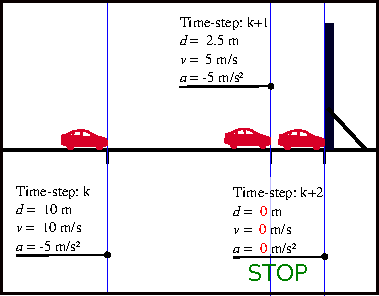
\includegraphics[width=0.7\linewidth]{\figurepath/car_example_2}
\caption{Braking phase for the car in scenario 1 as it stops before hitting the wall.}
\label{fig:car_example_2}
\end{figure}
Scenario 2: On a straight line, a second car is also  cruising towards the wall. Its current velocity is $v=10~m/s$, its distance to the wall is $d=10~m$ and its deceleration capability is $a_{m}=-1~m/s^2$. In its current state, none of the constraints\footnote{The constraint on its position ($d \geq 0$) and the constraint related to its deceleration capability ($a_m \leq a \leq a_M$).} of the car are violated. However, even if the vehicle starts \textit{braking} from time-step\footnote{For this example, the time-step duration is $1~s$.} $k$ using its full deceleration capability $a=a_{m}=-1~m/s$ (control input), collision with the wall is inevitable. Indeed, as shown in Fig.~\ref{fig:car_example_1}, during its braking phase, the car hits the wall between time-steps $k+1$ and $k+2$ and this, before bringing its velocity to $0$. In this case, it is said that: the constraint related to the deceleration capability of the car and the one on its position are \textit{incompatible}. At time-step $k+1$, there is no solution for the control problem that does not violate the car's constraints at the next time-step. \\
It is clear why there is no issue of constraints incompatibility for the vehicle in the first scenario as the amount of deceleration it can produce is larger than for the car in scenario 2, $-5~m/s^2$ compared to $-1~m/s^2$. A \labelText{{\color{red}\underline{solution}}}{label:solution} to ensure compatibility for the constraints of the vehicle in scenario 2 can be as follows: considering its low deceleration capability ($-1~m/s^2$), the black car in  Fig.~\ref{fig:car_example_1} should start \textit{braking} several time-steps in advance. Precisely, as shown in Fig.~\ref{fig:car_example_2}, $10$ time-steps before reaching the wall and $50~m$ from it. These are the needed time and distance to completely stop the vehicle considering an initial velocity of $v=10~m/s$. The only way to implement this solution is to reformulate the naive expression of the position related constraint to take into account the available deceleration capability $a_m$ in addition to the instantaneous state of the car plus the considered position limit: $f(d,v,a_{m})\geq 0$. With such a formulation, every time the vehicle reaches an \textit{extreme} state\footnote{An extreme state for the car is a state from which, considering its deceleration capability, if it starts braking using this maximum deceleration, it will stop just before hitting the wall.}, the reflected constraint on the control variable is automatically activated, a \textit{braking phase} is  implicitly engaged and a \textit{viable} \cite{aubin1991viability} solution is available for the control problem as the car copes with its position limit. 
\\
We recall the concept of \textit{viability} \cite{aubin2011viability} that is often used when dealing with the balance issue for humanoid robots. It can naturally be extended to the \textit{constraints incompatibility} problem \cite{fraichard2007short} as follows: \textit{A state is viable if starting from this state there exists over an infinite horizon of time a sequence of control inputs that satisfies all constraints in the future}. Therefore, considering the notion of \textit{viability}, unlike the state of the black car at time-step $k$ in scenario 1, the state of the red one in scenario 2 at the same time-step and for all the following time-steps is \textit{viable}. 
%\begin{landscape}
%\begin{figure}[!htbp]
%\centering
%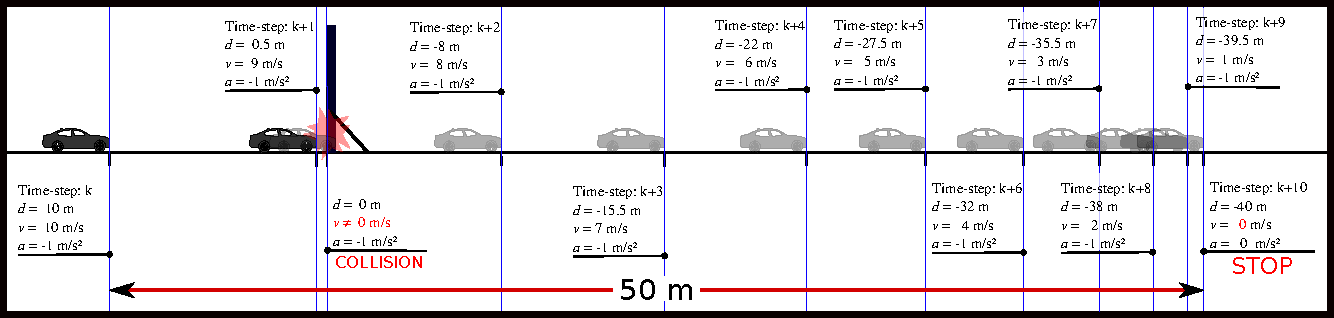
\includegraphics[width=0.99\linewidth]{\figurepath/car_example_1}
%\caption{Braking phase for the car in scenario 1 as it collides with the wall. Transparent frames show the continuation of the braking phase if the wall is removed.}
%\label{fig:car_example_1}
%\end{figure}
%\begin{table}[]
%\centering
%\begin{tabular}{|c|l|c|c|c|l|c|c|}
%\hline
%\multicolumn{4}{|c|}{Articular space constrains} & \multicolumn{4}{c|}{Operational space constraints} \\ \hline
%\multicolumn{2}{|c|}{\multirow{2}{*}{\begin{tabular}[c]{@{}c@{}}Type 1:\\ static constraints\\ $S \leq S_M$\end{tabular}}} & \multicolumn{2}{c|}{\begin{tabular}[c]{@{}c@{}}Dynamic constraints\\ $S \leq \~S_M$\end{tabular}} & \multicolumn{2}{c|}{\multirow{2}{*}{\begin{tabular}[c]{@{}c@{}}Type 4:\\ Static constraints\\ $g(S) \leq g_M$\end{tabular}}} & \multicolumn{2}{c|}{\begin{tabular}[c]{@{}c@{}}Dynamic constraints\\ $g(S) \leq \~g_M$\end{tabular}} \\ \cline{3-4} \cline{7-8} 
%\multicolumn{2}{|c|}{} & \begin{tabular}[c]{@{}c@{}}Type 2:\\ Predictable limit\\ $\~S_M$\end{tabular} & \begin{tabular}[c]{@{}c@{}}Type 3:\\ Non predictable limit\\ $\~S_M$\end{tabular} & \multicolumn{2}{c|}{} & \begin{tabular}[c]{@{}c@{}}Type 5:\\ Predictable limit\\ $\~g_M$\end{tabular} & \begin{tabular}[c]{@{}c@{}}Type 6:\\ Non predictable limit\\ $\~g_M$\end{tabular} \\ \hline
%\end{tabular}
%\caption{Types of constraints that can be encountered when using a reactive controller. $S=\{\vect{q}, \vect{\dot{q}}\}$ is the state of the robot in articular space. $g(S)$ is the mapping of this state in operational space.}
%\label{my-label}
%\end{table}
%\end{landscape}
\begin{landscape}
\begin{figure*}
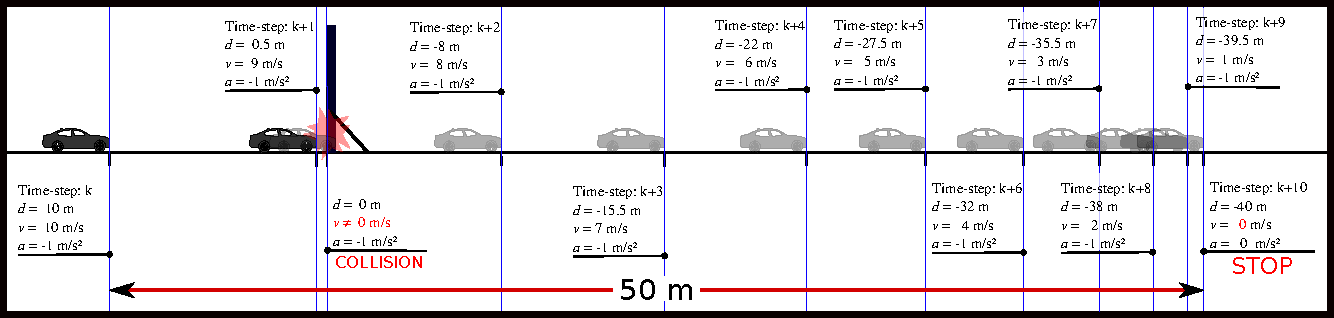
\includegraphics[width=1\linewidth]{\figurepath/car_example_1}
\caption{Braking phase for the car in scenario 2 as it collides with the wall. Transparent frames show the continuation of the braking phase in case the wall is removed.}
\label{fig:car_example_1}
\end{figure}
\begin{table}[]
\begin{center}
\begin{tabular}{|c|l|c|c|c|l|c|c|}
\hline
\multicolumn{4}{|c|}{Articular space constrains} & \multicolumn{4}{c|}{Operational space constraints} \\ \hline
\multicolumn{2}{|c|}{\multirow{2}{*}{\begin{tabular}[c]{@{}c@{}}Type 1:\\ static constraints\\ $S \leq S_M$\end{tabular}}} & \multicolumn{2}{c|}{\begin{tabular}[c]{@{}c@{}}Dynamic constraints\\ $S \leq \~S_M$\end{tabular}} & \multicolumn{2}{c|}{\multirow{2}{*}{\begin{tabular}[c]{@{}c@{}}Type 4:\\ Static constraints\\ $w(S) \leq w_M$\end{tabular}}} & \multicolumn{2}{c|}{\begin{tabular}[c]{@{}c@{}}Dynamic constraints\\ $w(S) \leq \~w_M$\end{tabular}} \\ \cline{3-4} \cline{7-8} 
\multicolumn{2}{|c|}{} & \begin{tabular}[c]{@{}c@{}}Type 2:\\ Predictable limit\\ $\~S_M$\end{tabular} & \begin{tabular}[c]{@{}c@{}}Type 3:\\ Non predictable limit\\ $\~S_M$\end{tabular} & \multicolumn{2}{c|}{} & \begin{tabular}[c]{@{}c@{}}Type 5:\\ Predictable limit\\ $\~w_M$\end{tabular} & \begin{tabular}[c]{@{}c@{}}Type 6:\\ Non predictable limit\\ $\~w_M$\end{tabular} \\ \hline
\end{tabular}
\caption{Types of constraints encountered when using a reactive controller. $S=\{\vect{q}, \vect{\dot{q}}, \vect{\ddot{q}}, \vect{\dddot{q}}\}$ is the extended state of the robot in articular space. $w(S)=\{\vect{X}, \vect{\dot{X}}, \vect{\ddot{X}}, \vect{\dddot{X}}\}$ is the mapping of this state in operational space.}
\label{my-label}
\end{center}
\end{table}
\end{landscape}
\subsection{Different types of constraints}
For reactive control schemes, types of constraints that can be encountered are summarized in table~\ref{my-label}. We distinguish two groups of constraints: 1) articular space constraints that concern directly the extended state of the robot $S=\{\vect{q}, \vect{\dot{q}}, \vect{\ddot{q}}, \vect{\dddot{q}}\}$. For example, the constraints related to an actuator's position and velocity limits. And 2) operational space constraints usually expressed as non-linear functions of $S$ and that relate to the movements of the robot in operational space. For example, a constraint of keeping a safe distance $d_{safe}$ between the robot and an obstacle within its workspace. Such constraint can, independently from other constraints, be expressed: 
\begin{equation}
\underbrace{\left(J_{c}(\vect{q}) \vect{\dot{q}}\right) }_{\dot{X}} \vec{\vect{n}} \hspace{1mm}\delta t + d \geq d_{safe},
\label{eq:bat_coll}
\end{equation}
where $J_c$ is the Jacobian matrix associated to the closest part from the structure of the robot to the obstacle, $\vec{\vect{n}}$ is the vector associated to the shortest distance between the obstacle and the robot, $\vect{\dot{q}}$ is the generalised articular velocity, $\delta t$ is the control sample-time and $d$: the instantaneous closest distance between the robot and the considered obstacle.
\\
As shown in table~\ref{my-label}, constraints from the two groups are either static or dynamic. A static constraint is a constraint which limit is constant and does not variate over time, for example, a physical position limit for an actuator. On the other hand, dynamic constraints are formulated with limits that can change in time, for example based on sensory acquired data. Variations of these limits can be either: 1) predictable, for example, a constraint of keeping a safe distance between the robot and an obstacle entering its workspace with a \textit{constant} velocity, 2) non-predictable, like the movement of a human-operator nearby the robot. The variation of the distance between the robot and the person cannot easily be predicted. \\
To prevent a robot from getting into \textit{non-viable} states, all its constraints must be reformulated to include the reaction capabilities of its actuators, namely: the max/min producible articular deceleration/torque and jerk. Analogue to the cars in scenarios 1 and 2, coping with a constraint implies a braking phase that is implicitly induced by the actuators of the robot. The span of such braking phase depends on the system's dynamic capabilities. Therefore, each constraint in table~\ref{my-label}, expressed with its naive formulation, can be compatible with the reaction capabilities of the robot in case of actuators that can produce infinite torque/deceleration and jerk. In such case, the duration of the implicitly induced braking phases can be reduced to \textbf{one} control sample-time. \\
The naive expressions of constraints in table~\ref{my-label} can be modified as follows:\\
For type 1 constraints, just as the suggested \nameref{label:solution} for the black car in scenario 2, considering constant articular  deceleration and jerk capabilities\footnote{Which is not exactly the case for multi-body robots.} and a static limit $S_M$, a \textit{formal} solution to the control problem that preserves \textit{viability} for the state of the robot can be computed. For this, the formulation of this type of constraints must be modified to take into account the system's articular reaction capabilities, namely, producible articular deceleration $[\vect{\ddot{q}}_m, \vect{\ddot{q}}_M]$ and jerk $[\vect{\dddot{q}}_m, \vect{\dddot{q}}_M]$. The same can also be done in case of constraints with dynamic predictable limits $\~S_M$ (type 2). Considering an accurate prediction, such bounds can be handled as static limits. For type 3 constraints, a straight forward solution is to widely bound the variations of the dynamic limit $\~S_M$, which can however substantially alter the optimality of the control solution regarding the task to perform. A type 3 constraint can be for example a constraint on the kinetic energy of the robot expressed in articular space. Such constraint can be formulated: $\frac{1}{2} M(\vect{q}) \vect{\dot{q}}^2 \leq E_c^{art}$, with $E_c^{art}$ the maximum allowed kinetic energy in articular space. When reflected on $\vect{\dot{q}}$, the constraint is written: $\vect{\dot{q}} \leq \sqrt{2 M(\vect{q})^{-1}E_c^{art}}$. The problem with constraints of type 4 is, even if the reaction capabilities of the robot in joint space can be considered constant, the non-linear and configuration dependent mapping\footnote{$[\vect{\ddot{q}}_m, \vect{\ddot{q}}_M], [\vect{\dddot{q}}_m, \vect{\dddot{q}}_M] \rightarrow [\vect{\ddot{X}}_m, \vect{\ddot{X}}_M], [\vect{\dddot{X}}_m, \vect{\dddot{X}}_M]$.} of these performances into operational space renders the estimation of the braking capabilities in Cartesian space impossible without predicting the future movements of the robot. Consequently, coping \textit{properly} with a static limit in Cartesian space is more complex. And it is even more for dynamic constraints (type 5 and type 6). A type 4 constraint can be for example a constraint on the operational velocity of the end-effector of a robotic manipulator. Such constraint can be expressed: $\vect{\dot{X}} = J(\vect{q}) \vect{\dot{q}} \leq \vect{\dot{X}}_M$, with $\vect{\dot{X}}_M$ the maximum allowed velocity for the end-effector in Cartesian space. A type 6 constraint can be for example a constraint on the operational velocity of end-effector of the robot but with a maximum allowed limit that depends on the instantaneous distance to a considered approaching obstacle. 
%This forecast of its future articular configurations as it brakes to cope with the considered constraints is important so the reaction capabilities in Cartesian space are guaranteed.
%For a constraint of type 1, just as the proposed solution for the car in scenario 1, to ensure viability, a formal solution that takes into account the articular\footnote{Considered constant.} reaction capabilities of the robot can be computed for the control problem; And this, in case the limit of the constraint is static or if it can be precisely predicted (type 2). DependiFng on these capabilities, the reflected constraint on the control input will be activated at the right time. \\
%For a type 3 constraint, a naive solution will be to widely bound the variations of its limit. This will however alter the optimality of the solution. The problem with constraints of type 4 is, even if the articular reaction capabilities can be considered constant\footnote{Which is not exactly the case for the articular deceleration and jerk capabilities.} in joint space, the non-linear and configuration dependent mapping of these performances in operational space makes the estimation of the braking profile impossible without any prediction on the future movements of the robot. Coping exactly with the static limit becomes a difficult task. Which is even more complex for dynamic constraints (type 5 and type 6).      
%In both articular and operational spaces, we distinguish static and dynamic constraints. A static constraint is a constraint which limit is constant and does not variate over time. On the other hand, dynamic constraints are formulated with limits that can change in time (for e.g. depending on sensory acquired data). 
%
%a constant limit in operational space corresponds actually to a dynamic one in articular space. This is due to the non-linear and configuration dependent mapping between the two domains. For example, a constraint of non-collision between the    
%%%%%%%%%%%%%%%%%%%%%%%%%%SUBSECTION%%%%%%%%%%%%%%%%%%%%%%%%%%%%%
%%%%%%%%%%%%%%%%%%%%%%%%%%%%%%%%%%%%%%%%%%%%%%%%%%%%%%%%%%%%%%%%%
%%%%%%%%%%%%%%%%%%%%%%%%%%SUBSECTION%%%%%%%%%%%%%%%%%%%%%%%%%%%%%
\subsection{Corresponding literature}
\label{subsec:crspnd_litt}
The problem of \textit{constraints incompatibility} in this chapter is tackled for constraints related to the articular position and velocity limitations of a robotic manipulator. Therefore, the brief state-of-the-art presented hereby is exclusive to the same type of constraints: (type 1 in table~\ref{my-label}). \\
The issue of \textit{constraints incompatibility} is studied in the literature since a long time and remains an open one. In \cite{park1998enhanced}, the problem of high peak of torque and chattering phenomena on the movement of the actuator is highlighted when a joint angle limit of a serial robot is reached. This results from decelerating the limiting joint in order to stop its motion in one sampling time. The following problems appear:
\begin{enumerate}
\item collision with the joint angle limit when no sufficient control torque and/or jerk capabilities are available.
\item vibrations by exciting hidden resonant modes of the manipulator which can lead to instability.
\end{enumerate}
Park et al. in \cite{park1998enhanced} use a method called \textit{P-Step-Ahead Predictor (PSAP)}. Articular position and velocity limits are  detected far earlier and the braking phases are activated $p$ time-steps in advance to reduce the required amount of torque. In addition, the modulation of a weighting matrix related to the manipulability measure \cite{yoshikawa1985manipulability} is used simultaneously for the same purpose. The problem with this proposed approach is the inevitable heuristic trial and error method to fix the acting parameters (e.g., $p$). Decr\'e et al. in \cite{decre2009extending} were the first to  formulate a mathematical solution to directly integrate the deceleration capabilities of a serial robot into the expression of a Cartesian position constraint aimed to keep the end-effector of a robot at a specific distance from the considered obstacle. Which results into a smoother articular velocity control input. Rubrecht et al. in \cite{rubrecht2010constraints} extend the idea to the constraints related to the articular limitations of a robotic manipulator. The deceleration capabilities are included in the formulation of the articular position constraint, that is then automatically activated $n$ time-steps before the joint position boundaries. However, only kinematic-level control is considered in their work. Lange in \cite{lange2014predictive} and  \cite{lange2015trajectory} use a scaling method to generate an immediate Path-Accurate and Jerk-Limited stopping motion for industrial robots. This method can at first glance be transposed and used when coping with articular limitations related constraints. The optimal time for triggering the stopping motion needs however to be computed.  \\

Besides these formal methods that have been proposed to solve the problem of constraints incompatibility, other techniques that are based on Optimal Control approaches seem well suited for handling that problem. Indeed, Optimal Control provides a systematic approach to optimally compute the control input so as to best track the control objectives while accounting for the current and future constraints on the control inputs and states of a system. As a matter of fact, to be able to guarantee the viability\footnote{As redefined as the very end of section 2.1.1.} of the state of the robot with respect to its articular constraints but also with respect to operational ones, the control problem should not be solved reactively but over an infinite horizon of time under these strict and explicit constraints.

Nevertheless, reasoning and solving the control problem over an infinite horizon of time does not make much sense in very dynamic environments and contexts where the tasks to be performed are defined and adapted on-line. This advocates for online Optimal Control approaches where the horizon of control input is recomputed at each control time step. However this comes at a very high price as it requires to employ a model of the system's dynamics in order to preview its behaviour over time and compute an optimal horizon of control inputs that maintain the system into a valid state space. It therefore requires a time-integration of the local system model which generally leads to costly non-linear and non-convex optimisation problems \cite{2016THDR3834}. In practice, to address this complexity problem, the time horizon can be reduced to some appropriate value. This falls in the category of Model Predictive Control where the Optimal Control problem is solved for a given receding horizon. While this reduces the computation cost, the latter remains high and one way to simplify it further is to use a reduced model of the system's dynamics in order to render the MPC problem simpler to solve. This approach has seen a lot of developments in the control of balance for humanoid robots where the dynamics of balancing are reduced to some more or less complex inverted pendulum control problem. This simplified model is used to compute, over a receding horizon, the desired acceleration of the center of mass of the robot given some path to follow and some balance constraints \cite{wieber2006trajectory}, \cite{ibanez2015Emergence}. While this model reduction approach leads to great results, it also implies a suboptimal use of the dynamics of the robot. Furthermore, the reduced model cannot not incorporate joint space variables which makes it impossible to actually account for very low-level constraints such as joint position limits or input torque saturation. 

MPC approaches are therefore gradually extended to control with the consideration of models capturing the system state at the joint level. Computational limitations nevertheless requires the setup of simplifications of the control problem. A significant improvement in this direction is performed by Y. Tassa et al.. in \cite{tassa2012synthesis}. The authors address computational issues in two ways in this work. First, the resolution of the MPC optimisation problem is considered over the whole duration of the activity. That is, the control problem solely aims at continuously driving the system towards an all-time minimum, rather than finding an optimum at each control step. To this aim a suboptimal solution solely is demanded at each control step, generally obtained through a single iteration of the optimisation algorithm. It therefore allows the consideration of much more complex optimisation problems. In this particular work, an iterative Linear Quadratic Gaussian optimiser, a variant of Differential Dynamic Programming, is setup to work over the joint actuation space. Computational issues nevertheless arise from the needs to update the model rapidly for an iteration of the optimiser. To meet this challenge, the second contribution of this work is thus to propose a fast dynamics integrator. However this controller still requires a large time slowdown with optimisation iterations of 140ms, thus forbidding a direct real-time implementation. The MPC problem is employed as a trajectory generator running slower than the rate of the lower, tracking control loop. This cannot be considered as satisfactory in terms of constraint compatibility but still provides an interesting step toward a general approach to this problem.

In this work, a different type of solution is explored and the choice is explicitly made to follow a formal approach, trying to exploit as much as possible formal compatibilisation of joint level imbricated constraints. The clear goal of such an approach is clearly to provide a very reactive way of keeping track of viability thus ensuring an optimal use of the system's dynamic capabilities.
%Besides these formal methods that have been proposed to solve the problem of \textit{constraints incompatibility}, other techniques that are based on Model Predictive Control (MPC) seem well suited for handling \textit{constraints incompatibilities}. Indeed, MPC provides a systematic approach to account for the current and future constraints on the control inputs and states of a system. In robotics, MPC is usually used as a common optimal approach for balance regulation. It employs a model of the system dynamics to preview its behaviour over time and compute an optimal horizon of control inputs that maintain the system into a valid state space. It requires therefore a time-integration of the local system model which generally leads to non-linear and non-convex optimisation problems \cite{ibanez:tel-01308723}. The formulation of the problem of \textit{constraints incompatibility} for constraints related to the physical articular limitations  of a robot controlled at the dynamic-level using MPC can be as:
%\begin{equation}
%\begin{split}
%\tau_{M}^c =\hspace{1mm} &\text{maximize  } \hspace{2.5mm}\tau_{|k}^c, \\
%&\text{subject to : }  S_{m_{|k}} \leq S_{|k} \leq S_{M_{|k}} \hspace{3mm} \forall k \in [0:\infty],
%\end{split}
%\label{eq:qddot_minimizkio}
%\end{equation}
%with $\tau^c$  the control torque input and $\tau_{M}^c$ its upper bound. $S_{|k}$, $S_{m_{|k}}$ and $S_{M_{|k}}$ are respectively the extended state of the robot expressed in articular space and its lower and upper bounds at control time-step $k$. The lower bound $\tau_{m}^c$ can similarly be computed by minimizing $\tau_{|k}^c$ rather than maximizing it. \\
%To be able to guarantee the \textit{viability}\footnote{As redefined in Section~\ref{sec:gen_prblm}.} of the state of the robot vis-a-vis its articular constraints, the problem described in (\ref{eq:qddot_minimizkio}) must be solved for an infinite horizon of time. However, computational limitations require the setup of simplifications of the control problem as time-integration is one of the major challenges of MPC formulations. A sliding finite horizon MPC strategy can then be preferred \cite{tan:tel-01310675}.
%A significant improvement in this direction was performed by Y. Tassa et al. in \cite{tassa2012synthesis} where the computational issues are addressed partially by considering the resolution of the MPC optimisation problem over just the whole duration of the activity instead of an infinite horizon of time.
%
%Because of these various limitations when using MPC and as a \textit{\textbf{formal}} solution to the \textit{constraints incompatibility} problem exist and can optimally be computed (especially regarding the constraints related to the physical articular limitations of a robotic manipulator). It is therefore the formal approach that is used in this chapter to resolve this problem for robots that are controlled at the dynamic-level.
%%%%%%%%%%%%%%%%%%%%%%%%%%SUBSECTION%%%%%%%%%%%%%%%%%%%%%%%%%%%%%
%%%%%%%%%%%%%%%%%%%%%%%%%%%%%%%%%%%%%%%%%%%%%%%%%%%%%%%%%%%%%%%%%
%%%%%%%%%%%%%%%%%%%%%%%%%%SUBSECTION%%%%%%%%%%%%%%%%%%%%%%%%%%%%%
\subsection{Contributions}
In this work, the problem of \textit{constraints incompatibility} is solved for constraints of type 1 and precisely for robots controlled at the dynamic-level. The constraints on articular positions, velocities, accelerations and jerk are expressed as inequalities within a QP formulation of a reactive control problem. The main contribution concerns the mathematical reformulation of the following constraints:
\begin{itemize}
\item no violation of joint position bounds;
\item no violation of joint velocity bounds.
\end{itemize}
To avoid incompatibility problems when reactively coping with such constraints, the new proposed formulations that are expressed at the dynamic-level take into account the reaction capabilities, i.e., the articular deceleration and jerk producible by the actuators of the robot. One kind of incompatibility can occur for example when a braking phase is implicitly induced by the actuators of the robot to stop the movement of a joint at a static position limit within a short period of time, for e.g., one control time-step. This requires high deceleration and jerk capabilities the robot may not be able to produce. Indeed, to be optimal, a robotic system must take the highest advantage from its dynamic capabilities within its limiting ranges; for example, to be as close as possible to a maximum allowed position with high articular acceleration and velocity and still be able to stop in time and not violate the considered limit. This can be achieved through a braking phase triggered $n$ time-steps before reaching the limit and that takes into account the system's limited available deceleration capabilities, i.e., the producible articular torque/deceleration and jerk. Every time an actuator reaches an \textit{extreme} state, with its new formulation, the constraint is activated and a braking phase is implicitly engaged at the right moment. In addition to the new formulations of the articular position and velocity constraints, that take into account the dynamic capabilities of the robot actuators. A method to compute the exact number $n$ of time-steps needed for the implicitly induced braking phases, triggered at the activation of the considered constraints, is introduced. The \textit{viability} of the state of the robot regarding the joint's position, velocity, acceleration/torque and jerk can then be guaranteed over an infinite horizon of time. \\
%In case of redundant manipulators, the control problem can either be formulated at the kinematic-level as the inversion of the following relation: 
%\begin{equation}
%\vect{\dot{X}} = J(\vect{q}) \dot{\vect{q}}
%\label{eq:vel_kin_opt}
%\end{equation}
%or at the torque-level when dynamic capabilities like contact forces control are needed: 
%\begin{equation}
%\vect{\ddot{X}} = \dot{J}(\vect{q}) \vect{\dot{q}} + J \ddot{\vect{q}}
%\label{eq:X_ddot}
%\end{equation}
%$J(\vect{q})$, $\vect{\dot{X}}$, $\vect{\ddot{X}}$, $\vect{\dot{q}}$, $\vect{\ddot{q}}$ are respectively the operational task Jacobian matrix, the operational velocity and acceleration vectors and the joint velocity and acceleration vectors.
%\\
%When it stills possible to implement constraints using an analytical scheme \cite{ngo2005passivity},\cite{ngo2006bounded}, the most general approach consists in formulating the control problem as a convex optimization one. Constraints are then expressed both through equalities and inequalities \cite{chen1994torque}-\cite{ma2002time}.
\\
The present chapter is organized as follows: In section 2, the reactive controller used to compare different formulations of the constraints on articular velocity and position is introduced. First, the naive formulations of these constraints are presented then, by studying the relation between the extended state of the robot $S=\{\vect{q}, \vect{\dot{q}}, \vect{\ddot{q}}\right), \vect{\dddot{q}}\}$ and the system's physical limitations: $[\vect{q}_m, \vect{q}_M]$, $[\vect{\dot{q}}_m, \vect{\dot{q}}_M]$, $[\vect{\ddot{q}}_m, \vect{\ddot{q}}_M]$, $[\vect{\dddot{q}}_m, \vect{\dddot{q}}_M]$, the different incompatibility cases that may occur are exposed. In section 3, the incompatibility cases are resolved and the new formulations of the joint velocity and position constraints that take into account the dynamic capabilities of the actuators of the robot are introduced. In section 4, the final bounds reflected on the dynamic control variable that allow coping with all a robotic manipulator's articular limitations at the same time are formulated. In section 5, the contributions are summarized, the encountered difficulties and the limitations of the proposed new formulation of constraints are highlighted. 
%In practical applications, a control strategy for a robotic system is usually formulated depending on the nature of the operational task to be performed. Two kinds of strategies are distinguished: a proactive one when the objective of the operational task is already known (e. g. moving the end-effector from point A to point B) and a reactive strategy when the input data for the operational task are not known a priori but discovered at every time-step (e.g., tele-operation, co-manipulation applications...etc.). 
%
%Independently from the control strategy, compliance to constraints and specifically to the physical constraints of the actuators is a must for any robotic system. This is particularly true in cases where constraints violation is highly critical (e.g., surgery, de-mining...etc.). 
%\\
%To ensure strict compliance, for proactive control strategies, constraints and tasks can be handled offline. For example, to move the end-effector from point A to point B in the Cartesian space, trajectories can be generated directly at the joint level. In this context, Katzschmann et. al in \cite{katzschmann2013towards} present a trajectory generating algorithm that takes into account the actuators max/min position, velocity, torque and even jerk capabilities. On the other hand, when tasks or constraints are not known in advance (reactive control cases), \textit{trajectories cannot be generated} and it becomes impossible to use the same approach to cope with articular limitations. In the presented work, this issue is solved for robots controlled at the dynamic-level. Constraints on articular positions, velocities, accelerations and jerk are expressed as inequalities within a QP formulation of the reactive control problem. The main contribution concerns the mathematical reformulation of the following constraints:
%\begin{itemize}
%\item No violation of joint position bounds.
%\item No violation of joint velocity bounds.
%\end{itemize}
%Within the new formulations, articular deceleration and jerk capabilities are integrated to avoid incompatibilities. One kind of incompatibilities can occur when inducing a braking phase to stop the movement of an actuator at a static\footnote{We distinguish two types of bounds/constraints: \begin{itemize}
%\item Static constraints: $x \leq x_{max}$ with: $x_{max}$ constant. 
%\item Dynamic constraints: $x \leq \~{x}_{max}(t)$ with: $\~x_{max}(t)$ varying over time.
%\end{itemize}
%}
%position limit within a short period of time, e.g., one control time-step. This requires high deceleration and jerk capabilities that the robot may not be able to produce. Indeed, to be optimal, a robotic system must take the highest advantage of its dynamic capabilities within its limiting ranges. For example, to be as close as possible to a maximum allowed position with high articular acceleration and velocity and still be able to stop at time and not violate the considered limit. This can be achieved through a braking phase triggered $n$ time-steps before reaching the limit and that takes into account the available deceleration capabilities of the system, namely: torque and jerk.  \\
%In case of redundant manipulators, the control problem can either be formulated at the kinematic-level as the inversion of the following relation: 
%\begin{equation}
%\vect{\dot{X}} = J(\vect{q}) \dot{\vect{q}}
%\label{eq:vel_kin_opt}
%\end{equation}
%or at the torque-level when dynamic capabilities like contact forces control are needed: 
%\begin{equation}
%\vect{\ddot{X}} = \dot{J}(\vect{q}) \vect{\dot{q}} + J \ddot{\vect{q}}
%\label{eq:X_ddot}
%\end{equation}
%$J(\vect{q})$, $\vect{\dot{X}}$, $\vect{\ddot{X}}$, $\vect{\dot{q}}$, $\vect{\ddot{q}}$ are respectively the operational task Jacobian matrix, the operational velocity and acceleration vectors and the joint velocity and acceleration vectors.
%\\
%When it stills possible to implement constraints using an analytical scheme \cite{ngo2005passivity},\cite{ngo2006bounded}, the most general approach consists in formulating the control problem as a convex optimization one. Constraints are then expressed both through equalities and inequalities \cite{chen1994torque}-\cite{ma2002time}. The issue of constraints compatibility exists since a long time and remains an open one. In \cite{park1998enhanced} the problem of high peak of torques and chattering phenomena is highlighted when the joint angle limit of a serial robot is reached. This results from decelerating the limiting joint in order to stop the motion in one sampling time. the following problems appear:
%\begin{enumerate}
%\item Collision with the joint angle limit when no sufficient control torque and/or jerk capabilities are available.
%\item Vibrations by exciting hidden resonant modes of the manipulator which can lead to instability.
%\end{enumerate}
%Park et al. in \cite{park1998enhanced} use a method called \textit{P-Step-Ahead Predictor (PSAP)}. Articular position and velocity limits are  detected far earlier and the braking phase is activated $p$ time-steps in advance to reduce the required amount of torque. In addition, the modulation of a weighting matrix related to the manipulability measure \cite{yoshikawa1985manipulability} can be used for the same purpose. The problem with the proposed approach is the inevitable heuristic trial and error method to fix the acting parameters (e.g., $p$). Decré et al. in \cite{decre2009extending} were the first to  formulate a mathematical solution to directly integrate the deceleration capabilities into the expression of a Cartesian position constraint; This resulted into a smoother articular velocity control input. Rubrecht et al. in \cite{rubrecht2010constraints} extended the idea to articular constraints. The deceleration capabilities  are integrated in the formulation of articular position constraints that are automatically activated $n$ time-steps before the joint position boundaries. Lange in \cite{lange2014predictive} and Suppa in \cite{lange2015trajectory} use a scaling method to generate an immediate Path-Accurate and Jerk-Limited stopping motion for industrial robots. This method can be transposed and used when coping with articular limits. The correct time for triggering the stopping motion needs however to be computed. 
%\\
%\\
%The organization of this chapter is as following: In section 2 we present the reactive controller that will be used to compare different formulations of articular constraints. We present the classic way used to formulate these constraints then, by studying the relationship between the joint parameters: $\vect{q}$, $\vect{\dot{q}}$, $\vect{\ddot{q}}$ and their corresponding limitations: $[\vect{q}_m, \vect{q}_M]$, $[\vect{\dot{q}}_m, \vect{\dot{q}}_M]$, $[\vect{\ddot{q}}_m, \vect{\ddot{q}}_M]$, $[\vect{\dddot{q}}_m, \vect{\dddot{q}}_M]$, we expose the different incompatibility cases that may occur. In section 3, the incompatibility cases are resolved and new formulations of velocity and position constraints that take into account the reaction capabilities of the robot are presented. 
%In section 4 we formulate the final bounds reflected on the control variable to cope with all the articular limits of the system at the same time. In section 5 we conclude and give more insights on the generalisation of the presented formulations for constraints expressed in the Cartesian space. 
%%%%%%%%%%%%%%%%%%%%%%%%%%%%%%%%%%%%%%%%%%%%%%%%%%%%%%%%%
      %The QP form and Constraints Compatibility%
%%%%%%%%%%%%%%%%%%%%%%%%%%%%%%%%%%%%%%%%%%%%%%%%%%%%%%%%%
\section[The QP form and the different constraints incompatibility cases]{The QP form and the different constraints incompatibility cases}
This section aims at establishing the general formulation of the constrained, redundant dynamic reactive control scheme. The objective is to compute every  time-step the control torque $\boldsymbol{\tau}_{|k}^{c}$ in order to perform a trajectory tracking task in joint space while coping at the same time with the articular position, velocity, torque/acceleration and jerk constraints. We highlight the fact that, desired trajectories for the joints of the robot are not known in advance but \textit{discovered at every time-step} (tele-operation analogue situation). Incompatibility cases related to the naive way of expressing the articular constraints are exposed and discussed. 
%%%%%%%%%%%%%%%%%%%%%%%%%%SUBSECTION%%%%%%%%%%%%%%%%%%%%%%%%%%%%%
%%%%%%%%%%%%%%%%%%%%%%%%%%%%%%%%%%%%%%%%%%%%%%%%%%%%%%%%%%%%%%%%%
%%%%%%%%%%%%%%%%%%%%%%%%%%SUBSECTION%%%%%%%%%%%%%%%%%%%%%%%%%%%%%
\subsection{Task formulation}
The objective function of the controller is defined as an error to be minimized. A joint-space acceleration task is considered and the error is between the desired articular acceleration $\vect{\ddot{q}}^{~des}$ and the expected acceleration $\vect{\ddot{q}}^{c}$; $\vect{\ddot{q}}^{~des}$ is computed:
\begin{equation}
\vect{\ddot{q}}_{|k}^{~des} = K_p (\vect{q}_{|k}^{*}-\vect{q}_{|k}) - K_d \vect{\dot{q}}_{|k}^{*}, 
\label{qddot}
\end{equation}
where $K_p$, $K_d$ $\in \mathbb{R}^{+}$ are the proportional and derivative gains.
%
%It is written in function of the control input $\vect{\tau}_{|k}^{c}$:
%\begin{equation}
% \vect{\ddot{X}}^{c} = J(\vect{q}) M(\vect{q})^{-1} \left(\boldsymbol{\tau}_{|k}^{c} - \vect{b}(\vect{q},\vect{\dot{q}})\right) + \dot{J}(\vect{q}) \vect{\dot{q}}
%\label{Xddot}
%\end{equation}
%$\vect{b}(\vect{q},\vect{\dot{q}})$ are the non linear terms, namely gravity, Coriolis and centrifugal induced generalized forces. $M(\vect{q})$ is the joint space inertia matrix of the robot. $\vect{\ddot{X}}^c$ can be computed with a PD controller to track a desired trajectory (position $\vect{X}(t)^\star$ and velocity  $\vect{\dot{X}}(t)^\star$, \textit{discovered at every time-step}). 
The acceleration task function to be minimized is written:
\begin{equation}
\vect{g}(\vect{\ddot{q}}_{|k}^{c}) = \vect{\ddot{q}}_{|k}^{~des}-\vect{\ddot{q}}_{|k}^c.
\label{artaccelerationError}
\end{equation}
%%%%%%%%%%%%%%%%%%%%%%%%%%SUBSECTION%%%%%%%%%%%%%%%%%%%%%%%%%%%%%
%%%%%%%%%%%%%%%%%%%%%%%%%%%%%%%%%%%%%%%%%%%%%%%%%%%%%%%%%%%%%%%%%
%%%%%%%%%%%%%%%%%%%%%%%%%%SUBSECTION%%%%%%%%%%%%%%%%%%%%%%%%%%%%%
\subsection{Controller formulation}
\label{subsec:cntrl_frm}
The proposed control strategy computes the control torque by minimizing the norm of the articular acceleration task function expressed in the following quadratic form: 
\begin{equation}
\argmin \limits_{\boldsymbol{\tau}_{|k}^{c}, \vect{\ddot{q}}_{|k}^{c}}  \left\| \vect{g}\left(\vect{\ddot{q}}_{|k}^{c}\right) \right\|_{Q_t}^2 + \epsilon  \| \boldsymbol{\tau}_{|k}^{c} \|_{Q_r}^2,
\label{eq:ctrl_pb}
\end{equation}
subject to:
\begin{equation}
M(\vect{q}_{|k}) \vect{\ddot{q}}_{|k}^{c} + \vect{b}(\vect{q}_{|k},\vect{\dot{q}}_{|k}) = \vect{\tau}_{|k}^{c},
\label{eq:dyn_eq}
\end{equation}
%subject to (\ref{eq:qddot_FINAL_CONSTR_1}) and (\ref{eq:qddot_FINAL_CONSTR_2}).
\\
with $\vect{\ddot{q}}_{|k}^{c}$ and $\vect{\tau}_{|k}^{c}$: the optimization control variables.
$\vect{b}(\vect{q}_{|k},\vect{\dot{q}}_{|k})$ are the non linear terms, namely gravity, Coriolis and centrifugal induced generalized forces. $M(\vect{q}_{|k})$ is the joint space inertia matrix of the robot. $Q_t$ and $Q_r$ are  positive semi-definite weighting matrices and $\| \vect{a} \|_{Q}$ is the $Q-$weighted euclidean norm of $a$. $\epsilon  \| \boldsymbol{\tau}_{|k}^{c} \|_{Q_r}^2$ with $\epsilon << 1$ serves as a regularization task in order to ensure the uniqueness of the control solution and to minimize the norm of the computed control torque.\\
It can be shown that the quadratic forms composing the tasks can be written as functions of positive semi-definite matrices. This LQP optimization problem is therefore convex and admits a unique global solution \cite{boyd2004}. 
\\ 
In addition to the equality constraints corresponding to the dynamic equation \eqref{eq:dyn_eq}, the problem is also subject to inequality constraints described in the upcoming sections. 
%
%\section{The QP form and articular constraints incompatibility cases}
%This section aims at establishing the general formulation of the constrained, redundant dynamic reactive control scheme. The objective is to compute the control torque $\boldsymbol{\tau}_{|k}^{c}$ in order to perform a trajectory tracking task in joint space while coping at every time-step with articular position, velocity, acceleration and jerk constraints. We highlight the fact that in this particular case the desired trajectories for the joint of the robot are \textit{discovered at every time-step} (tele-operation analogue situation) and are not known in advance. Incompatibility cases related to the classic way of expressing articular constraints are discussed. 
%\subsection{Task formulation}
%The objective function of the controller is defined as an error to be minimized. A joint-space acceleration controller is considered and the error is between the expected acceleration $\vect{\ddot{q}}^c$ and the real acceleration $\vect{\ddot{q}}$ of the robot's end-effector. It is written in function of the control input $\vect{\tau}_{|k}^{c}$:
%\begin{equation}
% \vect{\ddot{X}}^{c} = J(\vect{q}) M(\vect{q})^{-1} \left(\boldsymbol{\tau}_{|k}^{c} - \vect{b}(\vect{q},\vect{\dot{q}})\right) + \dot{J}(\vect{q}) \vect{\dot{q}}
%\label{Xddot}
%\end{equation}
%$\vect{b}(\vect{q},\vect{\dot{q}})$ are the non linear terms, namely gravity, Coriolis and centrifugal induced generalized forces. $M(\vect{q})$ is the joint space inertia matrix of the robot. $\vect{\ddot{X}}^c$ can be computed with a PD controller to track a desired trajectory (position $\vect{X}(t)^\star$ and velocity  $\vect{\dot{X}}(t)^\star$, \textit{discovered at every time-step}). The acceleration task function to be minimized is written:
%\hspace{-2mm}
%\begin{equation}
%\resizebox{.911\hsize}{!}{$\vect{g}\left(\boldsymbol{\tau}_{|k}^{c},\vect{\ddot{X}}^c\right) =  \vect{\ddot{X}}^c - \left(J(\vect{q}) M(\vect{q})^{-1} \left(\boldsymbol{\tau}_{|k}^{c} - \vect{b}(\vect{q},\vect{\dot{q}}) \right) + \dot{J}(\vect{q}) \vect{\dot{q}}\right)$}
%\label{accelerationError}
%\end{equation}
%\subsection{Controller formulation}
%The proposed control strategy computes the control torque by minimizing the norm of the  Cartesian acceleration task function expressed in the following quadratic form: 
%\begin{equation}
%\argmin \limits_{\boldsymbol{\tau}_{|k}^{c}}  \left\| \vect{g}\left(\boldsymbol{\tau}_{|k}^{c},\vect{\ddot{X}}^c\right) \right\|_{Q_t}^2 + \epsilon  \| \boldsymbol{\tau}_{|k}^{c} \|_{Q_r}^2,
%\label{eq:ctrl_pb}
%\end{equation}
%%subject to (\ref{eq:qddot_FINAL_CONSTR_1}) and (\ref{eq:qddot_FINAL_CONSTR_2}).
%\\
%$Q_t$ and $Q_r$ are  positive semi-definite weighting matrices and $\| \vect{a} \|_{Q}$ is the $Q-$weighted euclidean norm of $a$. $\epsilon  \| \boldsymbol{\tau}_{|k}^{c} \|_{Q_r}^2$ with $\epsilon << 1$ serves as a regularization task in order to ensure the uniqueness of the control solution and to minimize the norm of the computed control torque. It can be shown that the quadratic forms composing the tasks can be written as functions of positive semidefinite matrices. This LQP optimization problem is therefore convex and admits a unique global solution. 
%$\vect{\ddot{q}}_{|k}^{c}$ and $\vect{\tau}_{|k}^{c}$ are the control optimization variables: 
%\begin{equation}
%M(\vect{q}) \vect{\ddot{q}}_{|k}^{c} + \vect{b}(\vect{q},\vect{\dot{q}}) = \vect{\tau}_{|k}^{c}
%\label{eq:dyn_eq}
%\end{equation}
%\\ 
%In addition to the equality constraints corresponding to the dynamic equation \eqref{eq:dyn_eq}, the problem is also subject to inequality constraints described in the upcoming sections. 
%%%%%%%%%%%%%%%%%%%%%%%%%%SUBSECTION%%%%%%%%%%%%%%%%%%%%%%%%%%%%%
%%%%%%%%%%%%%%%%%%%%%%%%%%%%%%%%%%%%%%%%%%%%%%%%%%%%%%%%%%%%%%%%%
%%%%%%%%%%%%%%%%%%%%%%%%%%SUBSECTION%%%%%%%%%%%%%%%%%%%%%%%%%%%%%
\subsection{Articular constraints: naive formulations}
First, we introduce some notations that will be used throughout the manuscript:
\begin{itemize}
\item t $\in \mathbb{R}^{+}$ denotes time;
\item $k \in \mathbb{N}$ denotes the current discrete time-step;
\item $\delta t$ is the time-step duration of the discrete-time controller;
\item $\textit{S}_{|k}=\{\vect{q}_{|k}, \vect{\dot{q}}_{|k}, \vect{\ddot{q}}_{|k}, \vect{\dddot{q}}_{|k}\}$ is the extended state of the system at the current time-step $k$ describing its joint position, velocity, acceleration and jerk;
\item $[\vect{q}_{M}, \vect{q}_{m}]$ are the max/min joint position boundaries;
\item $[\vect{\dot{q}}_{m}, \vect{\dot{q}}_{M}], [\vect{\ddot{q}}_{m}, \vect{\ddot{q}}_{M}], [\vect{\dddot{q}}_{m}, \vect{\dddot{q}}_{M}]$ are the joint velocity, acceleration and jerk boundaries.
\end{itemize}
A naive satisfaction of the constraints related to these boundaries can be stated as: the computed control input $\boldsymbol{\tau}_{|k}^{c}$ at instant $k$ must be such that the articular limits are not violated at the next time-step $k+1$. These constraints can naturally be expressed in form of inequalities:
\begin{subequations}
\label{eq:const_1_literature}
\begin{empheq}[left={}\empheqlbrace]{align}
\vect{q}_{m} & \leq \vect{q}_{|k+1}\leq \vect{q}_{M},\label{eq:cnt_lit_1}\\
\vect{\dot{q}}_{m} & \leq \vect{\dot{q}}_{|k+1} \leq \vect{\dot{q}}_{M},\label{eq:cnt_lit_2}\\    
\vect{\ddot{q}}_{m} & \leq \vect{\ddot{q}}_{|k}^{c}\hspace{4mm}\leq \vect{\ddot{q}}_{M},\label{eq:cnt_lit_3}\\
\boldsymbol{\tau}_{m} & \leq \boldsymbol{\tau}_{|k}^{c}\hspace{4mm}\leq \boldsymbol{\tau}_{M},\label{eq:cnt_lit_4}\\
\vect{\dddot{q}}_{m}  & \leq \vect{\dddot{q}}_{|k+1}\leq \vect{\dddot{q}}_{M}.\label{eq:cnt_lit_5}
\end{empheq}
\end{subequations}
With $\boldsymbol{\ddot{q}}_m$ and $\boldsymbol{\ddot{q}}_M$ that can be computed as in Appendix~\ref{app:constrcomp}.
\\
To be easily accounted for, these constraints can be expressed in function of the control variable $\vect{\ddot{q}}_{|k}^{c}$. Considering the literature \cite{rubrecht2010constraints}, \cite{decre2009extending}, the classic approach to do that is based on the extended state of the system at instant $k$ and a local discrete linear approximation of its behaviour within a $\delta t$ time-step duration:  
%\begin{equation} 
%\left\{\begin{array}{l}
%\begin{split}
%\vect{q}_{|k+1} & = \vect{q}_{|k} + \delta t \vect{\dot{q}}_{|k} + \frac{\delta t^{2}}{2} \vect{\ddot{q}}_{|k},\\
%\vect{\dot{q}}_{|k+1} &  =  \vect{\dot{q}}_{|k} + \delta t \vect{\ddot{q}}_{|k},\\
%\vect{\dddot{q}}_{|k+1} &  =  \frac{1}{\delta t} (\vect{\ddot{q}}_{|k}^{c} - \vect{\ddot{q}}_{|k})
%\end{split}
%\end{array}\right.
%\label{eq:Constr_1_time_step}
%\end{equation}
\begin{subequations}
\label{eq:Constr_1_time_step}
\begin{empheq}[left={}\empheqlbrace]{align}
\vect{q}_{|k+1} & = \vect{q}_{|k} + \delta t \vect{\dot{q}}_{|k} + \frac{\delta t^{2}}{2} \vect{\ddot{q}}_{|k},\\
\vect{\dot{q}}_{|k+1} &  =  \vect{\dot{q}}_{|k} + \delta t \vect{\ddot{q}}_{|k},\\
\vect{\dddot{q}}_{|k+1} &  =  \frac{1}{\delta t} (\vect{\ddot{q}}_{|k}^{c} - \vect{\ddot{q}}_{|k}).
\end{empheq}
\end{subequations}
Note: for a torque control input $\vect{\tau}_{|k}^{c}$ computed for the current time-step $k$ and equivalent to an acceleration command $\vect{\ddot{q}}_{|k}^{c}$ \eqref{eq:dyn_eq}, the expected articular acceleration at the next time-step $k+1$ can be written: 
\begin{equation} 
\vect{\ddot{q}}_{|k}^{c} (input)  = \vect{\ddot{q}}_{|k+1} (output). 
\label{eq:cmd_input_dyn}
\end{equation}
Using (\ref{eq:Constr_1_time_step}), in case of a control at the dynamic-level (our case), constraints in (\ref{eq:const_1_literature}) can be reflected on the acceleration control variable $\vect{\ddot{q}}_{|k}^{c}$ as:
\begin{subequations}
\label{eq:Constr_time_step}
\begin{empheq}[left={}\empheqlbrace]{align}
\frac{2}{\delta t^2} (\vect{q}_{m}-\vect{q}_{|k}-\delta t \vect{\dot{q}}_{|k}) \leq & \hspace{1.5mm} \vect{\ddot{q}}_{|k}^{c} \leq \frac{2}{\delta t^2} (\vect{q}_{M}-\vect{q}_{|k}-\delta t \vect{\dot{q}}_{|k}),\label{eq:cnt_lit_tme_step_1}\\
\frac{1}{\delta t} (\vect{\dot{q}}_{m}-\vect{\dot{q}}_{|k}) \leq  & \hspace{1.5mm} \vect{\ddot{q}}_{|k}^{c} \leq \frac{1}{\delta t} (\vect{\dot{q}}_{M}-\vect{\dot{q}}_{|k}),\label{eq:cnt_lit_tme_step_2}\\
\vect{\ddot{q}}_{m} \leq & \hspace{1.5mm} \vect{\ddot{q}}_{|k}^{c} \leq \vect{\ddot{q}}_{M},\label{eq:cnt_lit_tme_step_3}\\
\vect{\dddot{q}}_{m} \delta t+\vect{\ddot{q}}_{|k} \leq  & \hspace{1.5mm} \vect{\ddot{q}}_{|k}^{c} \leq \vect{\dddot{q}}_{M} \delta t+\vect{\ddot{q}}_{|k}. \label{eq:cnt_lit_tme_step_4}
\end{empheq}
\end{subequations}
When these classic formulations are used, the reflected constraints (\ref{eq:Constr_time_step}) on $\vect{\ddot{q}}_{|k}^{c}$ are activated only one time-step before reaching the considered limits (i.e., \allowbreak$[\vect{q}_{M}, \vect{q}_{m}], [\vect{\dot{q}}_{m}, \vect{\dot{q}}_{M}], [\vect{\ddot{q}}_{m}, \vect{\ddot{q}}_{M}]$ and $[\vect{\dddot{q}}_{m}, \vect{\dddot{q}}_{M}]$). In such case, no sufficient time may be available for the actuators to react and cope with these  boundaries. The following \textbf{incompatibility cases} can appear and the control problem may become impossible to solve: 
\begin{enumerate}
\item \textbf{Incompatibility case related to the constraint on articular velocity:} 
Coping with a joint velocity constraint automatically implies bringing the articular acceleration $\vect{\ddot{q}}_{|k}$ to zero when hitting a max/min velocity limit $[\vect{\dot{q}}_{m}, \vect{\dot{q}}_{M}]$. In such case, an incompatibility problem may arise if no sufficient articular jerk can be produced by the actuator of the robot during the implicitly induced braking phase that brings the articular acceleration to zero. Coping at the same time with the articular velocity limit and the articular jerk limit may become impossible (see Fig.~\ref{fig:Constraints_incompatibility_vel_constr_JR}).
\begin{figure*}
\centering
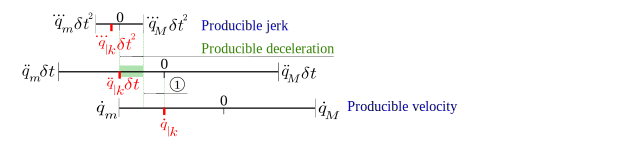
\includegraphics[width=1.0\columnwidth]{/home/anis/Desktop/THESIS_ANIS/THESIS/figures/Constrcomp/Constraints_incompatibility4_JR}
\caption{Extended state {\color{red} $S_{|k}$} of an articular joint moving towards its lower position limit $\vect{q}_m$ and one time-step before reaching its velocity limit $\vect{\dot{q}}_{m}$. The producible jerk is limiting the range from which the control variable $\vect{\ddot{q}}_{|k}^{c}$ can be picked: $\vect{\ddot{q}}_{|k}^{c}$ cannot be chosen equal to zero. Therefore, at the next time-step, at which $\vect{\dot{q}}_{|k}$ is equal to $\vect{\dot{q}}_{m}$, the articular acceleration cannot be brought to zero. The joint will continue to accelerate and the velocity limit will inevitably be violated. Because of the incompatibility with the producible jerk, it is impossible in this case to cope with the constraint on articular velocity. The incompatibility disappears if an actuator that can produce a larger amount of jerk is used: gape \circled{1} disappears.}
\label{fig:Constraints_incompatibility_vel_constr_JR}
\end{figure*}
\item \textbf{Incompatibility cases related to the joint position constraint:}
On the other hand, coping with a joint position constraint implies bringing both the articular velocity $\vect{\dot{q}}_{|k}$ and acceleration $\vect{\ddot{q}}_{|k}$ to zero when hitting the max/min position boundaries $[\vect{q}_{M}, \vect{q}_{m}]$. In this case, two incompatibility cases may arise: 
\begin{enumerate}[label=\Alph*]
\item \underline{The first} is when no sufficient articular deceleration is available during the implicitly induced braking phase (that lasts $1$ control time-step) even if sufficient braking jerk can be produced (see Fig.~\ref{fig:Constraints_incompatibility_posi_constr1}). 
\item \underline{The second} is when no sufficient jerk capabilities are available even if enough deceleration can be generated by the considered actuator (see Fig.~\ref{fig:Constraints_incompatibility_posi_constr2}).
\end{enumerate}
\begin{figure*}
\centering
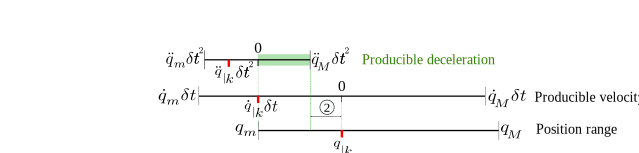
\includegraphics[width=1.0\columnwidth]{/home/anis/Desktop/THESIS_ANIS/THESIS/figures/Constrcomp/Constraints_incompatibility4_PC1}
\caption{Extended state {\color{red} $S_{|k}$} of an articular joint moving towards and one time-step before reaching its lower position limit $q_{m}$. The range of producible deceleration $\ddot{q}_{|k}^{c}$ is not sufficient to allow forcing the articular velocity to zero at the next time-step, at which $q_{|k}$ becomes equal to $q_m$. Because of the incompatibility with the deceleration capability, it is impossible in this case to satisfy the joint position constraint. This incompatibility disappears if an actuator that can produce a larger amount of  deceleration is used: gape \circled{2} disappears.}
\label{fig:Constraints_incompatibility_posi_constr1}
\end{figure*}
\begin{figure*}
\centering
\includegraphics[width=1.0\columnwidth]{/home/anis/Desktop/THESIS_ANIS/THESIS/figures/Constrcomp/Constraints_incompatibility4_PC2}
\caption{Extended state {\color{red} $S_{|k}$} of an articular joint moving towards and one time-step before reaching its lower position limit $q_{m}$. The producible jerk is limiting the range from which the control variable $\ddot{q}_{|k}^{c}$ can be picked: $\ddot{q}_{|k}^{c}$ cannot be chosen equal to zero. Therefore, it is not possible to force the articular velocity to zero for the next time-step, at which $q_{|k}$ becomes equal to $q_m$. Because of the incompatibility with the producible jerk, it is impossible in this case to cope with the joint position constraint. The incompatibility disappears if an actuator that can produce a larger amount of jerk is used: gape \circled{3} disappears.}
\label{fig:Constraints_incompatibility_posi_constr2}
\end{figure*}
\end{enumerate}
%%%%%%%%%%%%%%%%%%%%%%%%%%SUBSUBSECTION%%%%%%%%%%%%%%%%%%%%%%%%%%%%%
%%%%%%%%%%%%%%%%%%%%%%%%%%SUBSUBSECTION%%%%%%%%%%%%%%%%%%%%%%%%%%%%%
%\subsubsection{Incompatibility case related to the constraint on articular velocity}
%\label{subsubsec:inc_jnt_cnstr}
%Coping with a joint velocity constraint automatically implies bringing the articular acceleration $\vect{\ddot{q}}_{|k}$ to zero when hitting a Max/min velocity limit $[\vect{\dot{q}}_{m}, \vect{\dot{q}}_{M}]$. In such case, an incompatibility problem may arise if no sufficient articular jerk can be produced by the actuator of the robot during the implicitly induced braking phase that brings the articular acceleration to zero. Coping at the same time with the articular velocity limit and the articular jerk limit may become impossible (see Fig.~\ref{fig:Constraints_incompatibility_vel_constr_JR}).
%\begin{figure*}
%\centering
%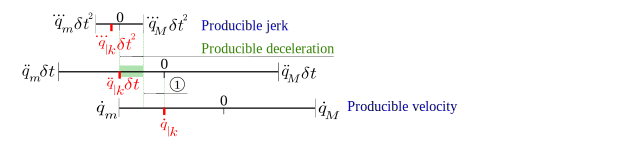
\includegraphics[width=1.0\columnwidth]{/home/anis/Desktop/THESIS_ANIS/THESIS/figures/Constrcomp/Constraints_incompatibility4_JR}
%\caption{Extended state {\color{red} $S_{|k}$} of an articular joint moving towards its lower position limit $\vect{q}_m$ and one time-step before reaching its velocity limit $\vect{\dot{q}}_{m}$. The producible jerk is limiting the range from which the control variable $\vect{\ddot{q}}_{|k}^{c}$ can be picked: $\vect{\ddot{q}}_{|k}^{c}$ cannot be chosen equal to zero. Therefore, at the next time-step, at which $\vect{\dot{q}}_{|k}$ is equal to $\vect{\dot{q}}_{m}$, the articular acceleration cannot be brought to zero. The joint will continue to accelerate and the velocity limit will inevitably be violated. Because of the incompatibility with the producible jerk, it is impossible in this case to cope with the constraint on articular velocity. The incompatibility disappears if an actuator that can produce a larger amount of jerk is used: gape \circled{1} disappears.}
%\label{fig:Constraints_incompatibility_vel_constr_JR}
%\end{figure*}
%%%%%%%%%%%%%%%%%%%%%%%%%%%SUBSUBSECTION%%%%%%%%%%%%%%%%%%%%%%%%%%%%%
%%%%%%%%%%%%%%%%%%%%%%%%%%%SUBSUBSECTION%%%%%%%%%%%%%%%%%%%%%%%%%%%%%
%\subsubsection{Incompatibility cases related to the joint position constraint}
%On the other hand, coping with a joint position constraint implies bringing both the articular velocity $\vect{\dot{q}}_{|k}$ and acceleration $\vect{\ddot{q}}_{|k}$ to zero when hitting the Max/min position boundaries $[\vect{q}_{M}, \vect{q}_{m}]$. In this case, two incompatibility cases may arise. The first is when no sufficient articular deceleration is available during the implicitly induced braking phase (that lasts $1$ control time-step) even if sufficient braking jerk can be produced (see Fig.~\ref{fig:Constraints_incompatibility_posi_constr1}). The second is when no sufficient jerk capabilities are available even if enough deceleration can be generated by the considered actuator (see Fig.~\ref{fig:Constraints_incompatibility_posi_constr2}).
%\begin{figure*}
%\centering
%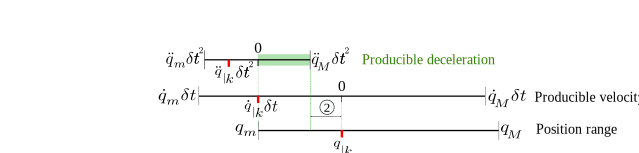
\includegraphics[width=1.0\columnwidth]{/home/anis/Desktop/THESIS_ANIS/THESIS/figures/Constrcomp/Constraints_incompatibility4_PC1}
%\caption{Extended state {\color{red} $S_{|k}$} of an articular joint moving towards and one time-step before reaching its lower position limit $q_{m}$. The range of producible deceleration $\ddot{q}_{|k}^{c}$ is not sufficient to allow forcing the articular velocity to zero at the next time-step, at which $q_{|k}$ becomes equal to $q_m$. Because of the incompatibility with the deceleration capability, it is impossible in this case to satisfy the joint position constraint. This incompatibility disappears if an actuator that can produce a larger amount of  deceleration is used: gape \circled{2} disappears.}
%\label{fig:Constraints_incompatibility_posi_constr1}
%\end{figure*}
%\begin{figure*}
%\centering
%\includegraphics[width=1.0\columnwidth]{/home/anis/Desktop/THESIS_ANIS/THESIS/figures/Constrcomp/Constraints_incompatibility4_PC2}
%\caption{Extended state {\color{red} $S_{|k}$} of an articular joint moving towards and one time-step before reaching its lower position limit $q_{m}$. The producible jerk is limiting the range from which the control variable $\ddot{q}_{|k}^{c}$ can be picked: $\ddot{q}_{|k}^{c}$ cannot be chosen equal to zero. Therefore, it is not possible to force the articular velocity to zero for the next time-step, at which $q_{|k}$ becomes equal to $q_m$. Because of the incompatibility with the producible jerk, it is impossible in this case to cope with the joint position constraint. The incompatibility disappears if an actuator that can produce a larger amount of jerk is used: gape \circled{3} disappears.}
%\label{fig:Constraints_incompatibility_posi_constr2}
%\end{figure*}
%%%%%%%%%%%%%%%%%%%%%%%%%%SUBSECTION%%%%%%%%%%%%%%%%%%%%%%%%%%%%%
%%%%%%%%%%%%%%%%%%%%%%%%%%%%%%%%%%%%%%%%%%%%%%%%%%%%%%%%%%%%%%%%%
%%%%%%%%%%%%%%%%%%%%%%%%%%SUBSECTION%%%%%%%%%%%%%%%%%%%%%%%%%%%%%
\section{Test case scenario for simulation}
In this section, the test case scenario used as a basis for testing all the different formulations of the constraints on articular velocity and position is presented. A comparison between the naive and new formulations will then be performed in Section~\ref{sec:art_cnstr_new_frml}. The controller described in Section~\ref{subsec:cntrl_frm} is implemented as a C++ Orocos component \cite{rtt-url} on a virtual model of the KUKA LWR4 serial robot using XDE, a robotics-oriented physics simulation engine \cite{merlhiot2012}. 

As a main activity, the robot performs a trajectory tracking task where its joints track desired articular positions \textit{(discovered at every time-step)} (see Fig.~\ref{fig:kuka_screen}). During its movement, the system is pushed to its physical limits (max/min articular positions, velocities, accelerations and jerks). The LQP is solved in real-time at a period of $1~ms$ using Gurobi, a commercial optimization software \cite{gurobi}. Values used for the gains of the controller during simulation are: $K_p=400$, $K_d=2\sqrt{K_p}$. $Q_t$ and $Q_r$ in this case are identity matrices. For demonstration purposes, only the physical capabilities of the first joint of the robot (joint $0$) are constrained. 
%As a main activity, the robot performs a trajectory tracking task where the end-effector tracks a desired position and orientation \textit{(discovered at every time-step)} in Cartesian space (see Fig.~\ref{fig:kuka_screen}). During its movement, the system is pushed to its physical limits (articular positions, velocities, accelerations and jerks). The LQP is solved in real time at a period of 1\textit{ms} using Gurobi, a commercial optimization software \cite{gurobi}. For demonstration purposes, only the physical capabilities of the first joint of the robot will be constrained. 
%The articular limitations are chosen as following: 
%$[q_{0_{m}}, q_{0_{M}}]=[,]$, $[\dot{q}_{0_{m}}, \dot{q}_{0_{M}}]=[,]$, $[\ddot{q}_{0_{m}}, \ddot{q}_{0_{M}}]=[,]$, $[\dddot{q}_{0_{m}}, \dddot{q}_{0_{M}}]=[,]$.  
\begin{figure}[!htbp]
\centering
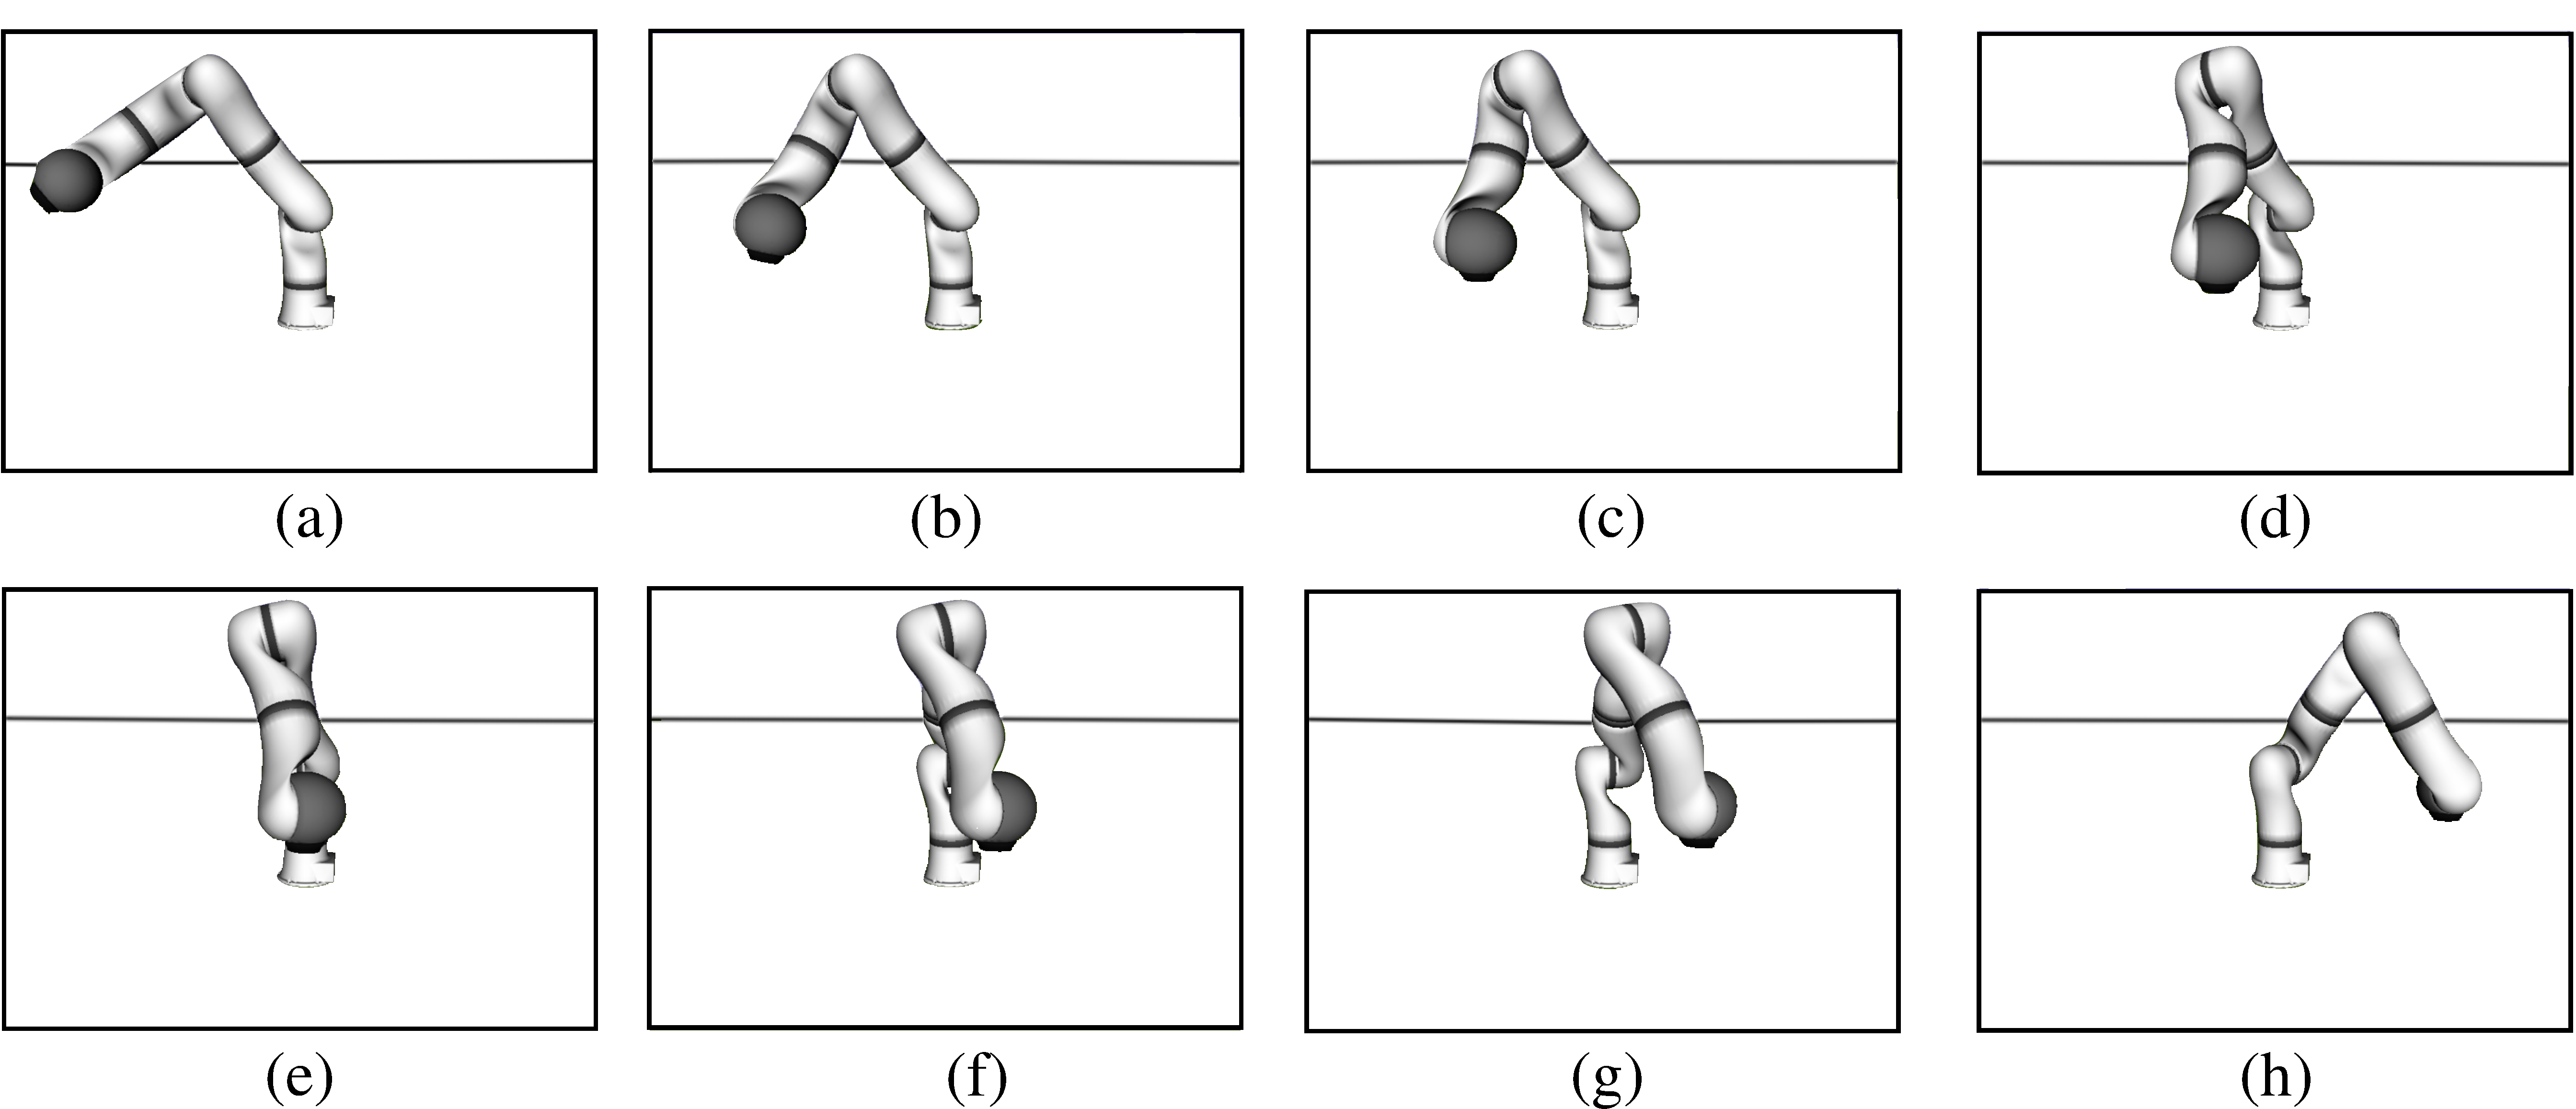
\includegraphics[width=1.0\columnwidth]{/home/anis/Desktop/THESIS_ANIS/THESIS/figures/Constrcomp/kuka_screen}
\caption{Screenshots of the test case scenario simulation with the KUKA LWR4 robot.}
\label{fig:kuka_screen}
\end{figure*}
\begin{figure}[!htbp]
\centering
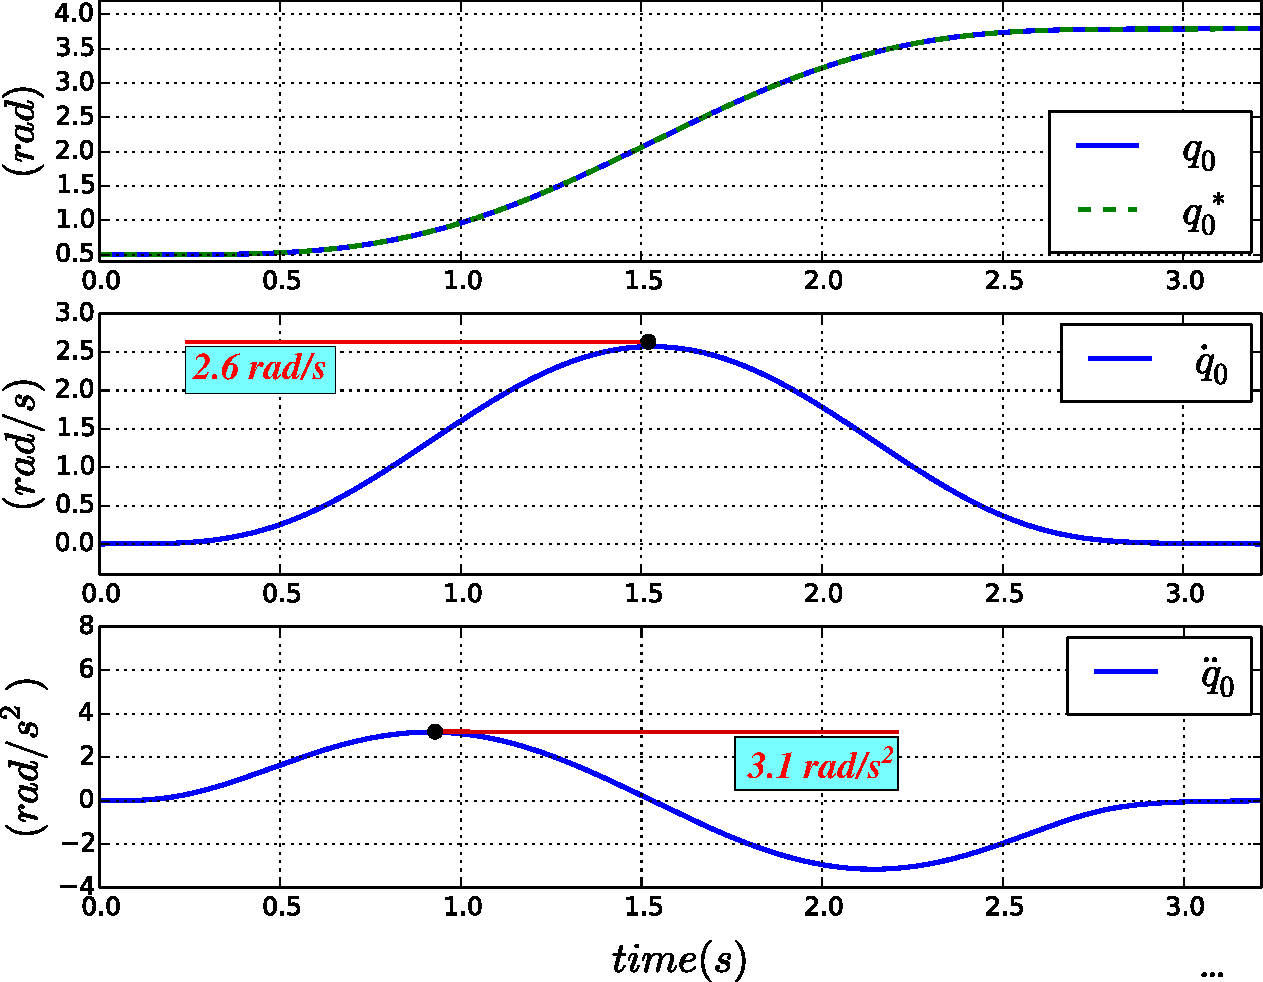
\includegraphics[width=0.8\columnwidth]{/home/anis/Desktop/THESIS_ANIS/THESIS/figures/Constrcomp/No_constr_move}
\caption{Extended state $S$ of joint $0$ during the test case scenario. The movement of the joint is not constrained. Top to bottom: position, velocity, acceleration and jerk.}
\label{fig:No_constr_move}
\end{figure}
\\
Fig.~\ref{fig:No_constr_move} shows the extended state of joint $0$ as it reaches its desired position $q_0^*=3.79~rad$\footnote{The position range for joint $0$ on a real KUKA LWR4 is $[q_{m_{0}}, q_{M_{0}}]=[-2.97, 2.97]~rad$. A wider domain is considered in simulation.} within $3.5~s$. During its movement, joint $0$ reaches a maximum velocity of $2.57~rad.s^{-1}$, a maximum acceleration of $3.15~rad.s^{-2}$ and a maximum jerk of $-8.05~rad.s^{-3}$.
%%%%%%%%%%%%%%%%%%%%%%%%%%%%%%%%%%%%%%%%%%%%%%%%%%%%%%%%%
       %Articular constraints: new formulations%
%%%%%%%%%%%%%%%%%%%%%%%%%%%%%%%%%%%%%%%%%%%%%%%%%%%%%%%%%                         
\section{Articular constraints: new formulations}
\label{sec:art_cnstr_new_frml}
In this section, the incompatibility cases previously exposed for the articular velocity and position constraints are resolved. The classic (naive) formulation of the articular velocity constraint is modified to include the actuators jerk capabilities. The naive expression of the joint position constraint on the other hand, is  reformulated to take into account both the amounts of deceleration and jerk producible by the actuators of the robot. Considering these reaction capabilities and compared to the cases where the naive formulations of the constraints are used, the braking phases \textit{implicitly induced} on the movements of a constrained articulation start earlier, and at the right time to cope with the different joint's physical limitations. Each incompatibility case is resolved as follows: first, the extended state $S$ of the joint during the \textit{implicitly induced} braking phase\footnote{Induced at the activation of the constraint.} is described then second, based on this description, the new formulations of the constraints on articular velocity and position are derived. Finally, the behaviour of the robot with the new formulations of the constraints is compared to its behaviour when the naive ones are used. 
%%%%%%%%%%%%%%%%%%%%%%%%%%SUBSECTION%%%%%%%%%%%%%%%%%%%%%%%%%%%%%
%%%%%%%%%%%%%%%%%%%%%%%%%%%%%%%%%%%%%%%%%%%%%%%%%%%%%%%%%%%%%%%%%
%%%%%%%%%%%%%%%%%%%%%%%%%%SUBSECTION%%%%%%%%%%%%%%%%%%%%%%%%%%%%%
\subsection{Joint velocity constraint incompatibility with jerk limits}
\label{subsec:jnt_vel_cnstr_inc_jerk}
As previously explained, the constraint on the articular velocity of the robot (\ref{eq:cnt_lit_tme_step_2}) and the one on its producible articular jerk (\ref{eq:cnt_lit_tme_step_4})
may become incompatible if a joint gets close to one of its velocity limits too fast (see Fig.~\ref{fig:Constraints_incompatibility_vel_constr_JR}). In  this case, admissible\footnote{Regarding either the dynamic capabilities of the actuator or the task to be performed by the robot.} jerk may not be sufficient to allow a quick variation of the articular torque and it becomes impossible to bring the articular acceleration to zero within only one control time-step. The only solution to preserve compatibility is to \textit{induce an implicit} braking phase with maximum jerk, several time-steps (not just one) before reaching the velocity boundary. The braking phase lasts therefore $(n_{1} \in \mathbb{N}\geq 1)$ control time-steps. 
\\
Lets consider the braking phase for a joint moving towards and reaching its maximum velocity limit $\dot{q}_{M}$. During this phase, the actuator brakes with constant jerk $\dddot{q}_{m} \leq 0$ until maximum velocity $\dot{q}_{M} \geq 0$ is attained. The extended state \textit{S} of the system during such phase can be described (Note that the upcoming calculations are performed for each joint of the robot. $q$, $\dot{q}$, $\ddot{q}$, $\dddot{q}$ respectively represent one of the components of $\vect{q}}$, $\vect{\dot{q}}$, $\vect{\ddot{q}}$, $\vect{\dddot{q}}$ (in bold)):
\begin{equation} 
\begin{split}
\textit{S}_{|k+1}&\left\{\begin{array}{lcl}
\dot{q}_{|k+1} \hspace{1mm}= \dot{q}_{|k} + \ddot{q}_{|k} \delta t, \\
\ddot{q}_{|k+1} \hspace{1mm}= \ddot{q}_{|k} + \dddot{q}_{m} \delta t;
\end{array}\right.\\
\textit{S}_{|k+2}&\left\{\begin{array}{lcl}
\dot{q}_{|k+2} \hspace{1mm}= \dot{q}_{|k+1} + \ddot{q}_{|k+1} \delta t, \\
\ddot{q}_{|k+2} \hspace{1mm}= \ddot{q}_{|k+1} + \dddot{q}_{m} \delta t;
\end{array}\right.\\
& \hspace{7mm}\vdots\ \hspace{12mm}\vdots\\\
\textit{S}_{|k+n_{1}}&\left\{\begin{array}{lcl}
\dot{q}_{|k+n_{1}} = \dot{q}_{|k+n_{1}-1} + \ddot{q}_{|k+n_{1}-1} \delta t, \\
%\vspace{2mm}
\ddot{q}_{|k+n_{1}} = \ddot{q}_{|k+n_{1}-1} + \dddot{q}_{m} \delta t.
\end{array}\right.
\end{split}
\label{eq:discretized_dynamics_vel}
\end{equation}
With: $\dot{q}_{|k} \geq 0$, $\ddot{q}_{|k} \geq 0$ and  $\dddot{q}_{m} \leq 0$. The joint velocity evolution in $n_1$ iterations is equal to the general form\footnote{Computed using Maple \cite{maple}.} of the numerical sequence (\ref{eq:discretized_dynamics_vel}):
\begin{equation}
\begin{split}
\dot{q}_{|k+n_1} = \dot{q}_{|k} + n_1 \ddot{q}_{|k} \delta t + \frac{(n_1^2-n_1)}{2} \dddot{q}_{m} \delta t^2.
\label{eq:q_dot_evolution_with_const_qdddot_m}
\end{split}
\end{equation}
In case of a control at the dynamic-level, considering (\ref{eq:cmd_input_dyn}), the condition $\dot{q}_{|k+n_1} \leq \dot{q}_{M}$ for all integer $n_1$ leads to:
\begin{equation}
\begin{split}
\ddot{q}_{|k}^{c} \leq \frac{(\dot{q}_M-\dot{q}_{|k})}{n_1 \delta t} - \frac{(n_1-1)}{2} \dddot{q}_m \delta t. 
\label{eq:q_ddot_vel_jerk_comp_aa_n1}
\end{split}
\end{equation}
With $n_1$, the integer minimizing the right-hand side of (\ref{eq:q_ddot_vel_jerk_comp_aa_n1}). By differentiating this expression w.r.t $n_1$:
\begin{equation} 
\hspace{-4mm}
\left. \begin{array}{r} 
n_1 \geq 1 \\
\myfrac[5pt]{-(\dot{q}_M-\dot{q}_{|k})}{n_1^2 \delta t} - \frac{\delta t}{2} \dddot{q}_m  = 0
\end{array} \right\} 
\Rightarrow n_1=-\myfrac[5pt]{\sqrt{-2\dddot{q}_m(\dot{q}_M-\dot{q}_{|k})}}{\dddot{q}_m \delta t}.
\label{eq:n_1_eq_aa}
\end{equation}
Following the same reasoning for the lower velocity limit, the condition $\dot{q}_{|k+n_2} \geq \dot{q}_{m}$ for all integer $n_2 \geq 1$ becomes: 
\begin{equation}
\begin{split}
\ddot{q}_{|k}^{c} \geq \frac{(\dot{q}_m-\dot{q}_{|k})}{n_2 \delta t} - \frac{(n_2-1)}{2} \dddot{q}_M \delta t.
\label{eq:q_ddot_vel_jerk_comp_aa_n2}
\end{split}
\end{equation}
With:
\begin{equation}
n_2 = \myfrac[5pt]{\sqrt{-2\dddot{q}_M(\dot{q}_m-\dot{q}_{|k})}}{\dddot{q}_M \delta t}, 
\label{eq:n_2_eq_aa}
\end{equation}
maximizing the right-hand side of (\ref{eq:q_ddot_vel_jerk_comp_aa_n2}). \\
$n_1$ is the number of time-steps corresponding to the span of a braking phase implicitly induced by an articulation moving towards its upper velocity limit $\dot{q}_{M}$, and during which its positive acceleration is brought to zero by jerking negatively with $\dddot{q}_m$; and $n_1$ is the number of time-steps corresponding to the span of a braking phase implicitly induced by an articulation moving towards its lower velocity limit $\dot{q}_{m}$, and during which its negative acceleration is brought to zero by jerking positively using $\dddot{q}_M$.\\
Finally, the reflected constraint on the acceleration control variable $\ddot{q}_{|k}^{c}$ is of the form: 
\begin{equation}
\begin{split}
f_{\beta}(\dot{q}_{|k}, \dot{q}_m, \dddot{q}_M, n_2) \leq \ddot{q}_{|k}^{c} \leq f_{\alpha}(\dot{q}_{|k}, \dot{q}_M, \dddot{q}_m, n_1), 
\label{eq:qddot_cond_to_satisfy_Jerk_Vel_compatibility_profile}
\end{split}
\end{equation}
with $f_{\beta}$ and $f_{\alpha}$ as in (\ref{eq:q_ddot_vel_jerk_comp_aa_n1}) and (\ref{eq:q_ddot_vel_jerk_comp_aa_n2}).
%********************************************************************%
\subsubsection{Illustration 1}
To illustrate this first theoretical result, in this simulation, using the test case scenario, joint $0$ moves towards its upper velocity limit $\dot{q}_{M_{0}}$. Only the classic (naive) formulation of the joint velocity constraint (\ref{eq:cnt_lit_tme_step_2}) is implemented with the controller: (\ref{eq:ctrl_pb}), (\ref{eq:dyn_eq}). The constraint on articular jerk (\ref{eq:cnt_lit_tme_step_4}) is not considered. 
%0
\begin{figure}[!htbp]
\centering
{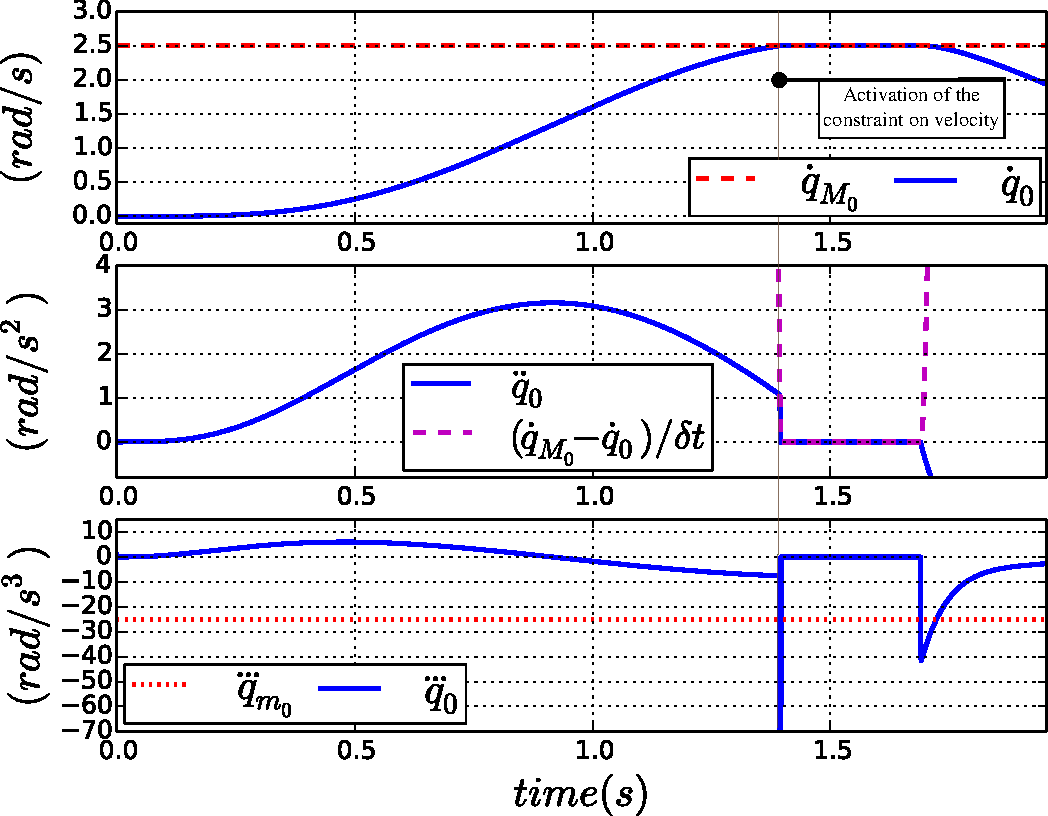
\includegraphics[width=0.8\columnwidth]{/home/anis/Desktop/THESIS_ANIS/THESIS/figures/Constrcomp/0_Vel_constr_classic}}
\caption{Extended state $S$ of joint $0$ during the braking phase (that lasts 1 control time-step $= 1~ms$) implicitly induced to cope with the maximum velocity limit $\dot{q}_{M_{0}}$. The naive formulation of the articular velocity constraint (\ref{eq:cnt_lit_tme_step_2}) is used. Top to bottom: velocity, acceleration and jerk.} 
\label{fig:0_Vel_constr_classic}
\end{figure}
Fig.~\ref{fig:0_Vel_constr_classic} shows the extended state of joint $0$ during a braking phase implicitly induced only one control time-step ($1~ms$) before reaching $\dot{q}_{M_{0}}$. A high peak of jerk is induced. In this case, if the constraint on articular jerk (\ref{eq:cnt_lit_tme_step_4}) is implemented in the controller's configuration, the control problem becomes impossible to solve. It is then clear that for a real system with limited jerk capabilities $($e.g., $\dddot{q}_{M_{0}} = 25~rad.s^{-3})$, coping with a velocity limit using the naive formulation of the articular velocity constraint is simply impossible. \\
On the other hand, when the new formulation of this constraint (\ref{eq:q_ddot_vel_jerk_comp_aa_n1}) is used, the system starts braking $n_1$ time-steps before reaching the velocity limit $\dot{q}_{M_0}$ (see Fig.~\ref{fig:1_Vel_constr_jerk_comp}). Joint $0$ is capable of coping at the same time with both its velocity and jerk limits (see Fig.~\ref{fig:1_Vel_constr_jerk_comp_zoom}). In this case, including the constraint on articular jerk (\ref{eq:cnt_lit_tme_step_4}) in the configuration of the controller will not result into an infeasible control problem. Therefore, the incompatibility between the articular velocity and jerk constraints is resolved.
%1
\begin{figure}[!htbp]
\centering
{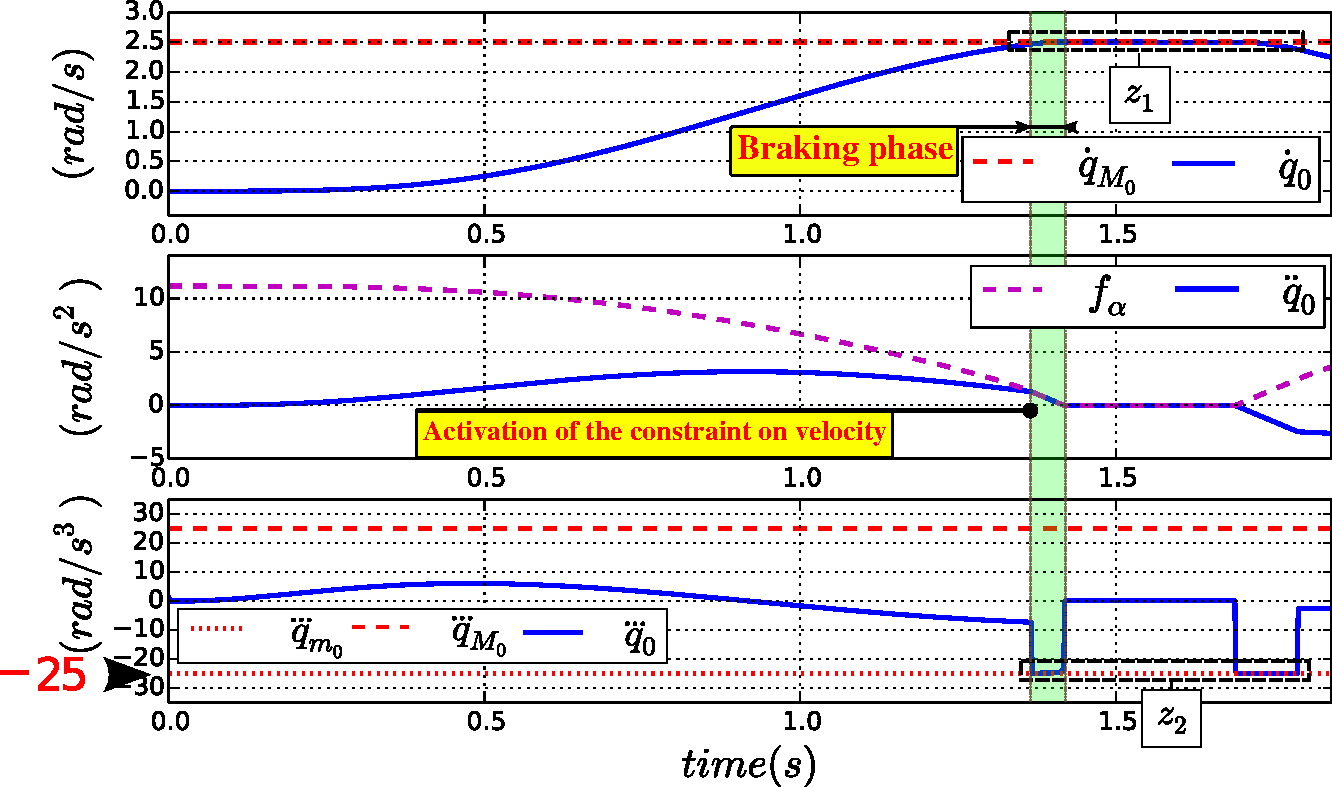
\includegraphics[width=0.9\columnwidth]{/home/anis/Desktop/THESIS_ANIS/THESIS/figures/Constrcomp/1_Vel_constr_jerk_comp_}}
\caption{Extended state $S$ of joint $0$ during the braking phase implicitly induced to cope with a maximum velocity limit $\dot{q}_{M_{0}}$. In this case, the new formulation of the constraint on articular velocity (\ref{eq:q_ddot_vel_jerk_comp_aa_n1}) that takes into account the actuator's maximum producible jerk $(\dddot{q}_{m_{0}} = 25~rad.s^{-3})$ is used. Note that $n_1$, is physically meaningful only during the span of the implicitly induced braking phase. Top to bottom: velocity, acceleration, jerk and $n_1$. $z_1$ and $z_2$ are in Fig.~\ref{fig:1_Vel_constr_jerk_comp_zoom}}. 
\label{fig:1_Vel_constr_jerk_comp}
\end{figure}
\begin{figure}[!htbp]
\centering
{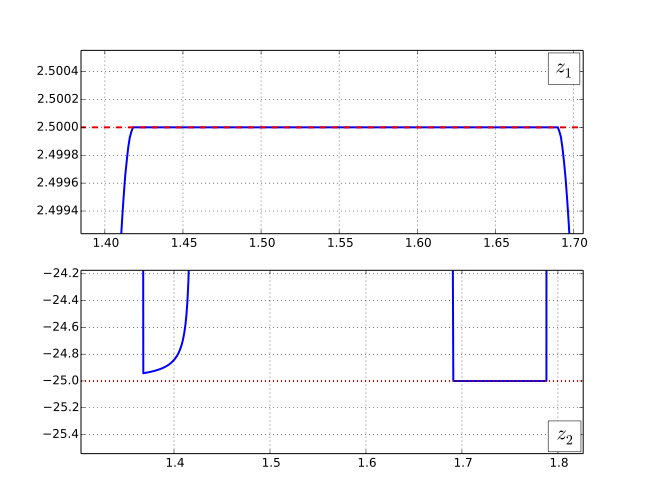
\includegraphics[width=0.8\columnwidth]{/home/anis/Desktop/THESIS_ANIS/THESIS/figures/Constrcomp/1_Vel_constr_jerk_comp_zoom}}
\caption{Zooms corresponding to Fig.~\ref{fig:1_Vel_constr_jerk_comp}.} 
\label{fig:1_Vel_constr_jerk_comp_zoom}
\end{figure}
%
%\begin{landscape}
%\begin{figure}
%\begin{minipage}[c]{0.48\linewidth}
%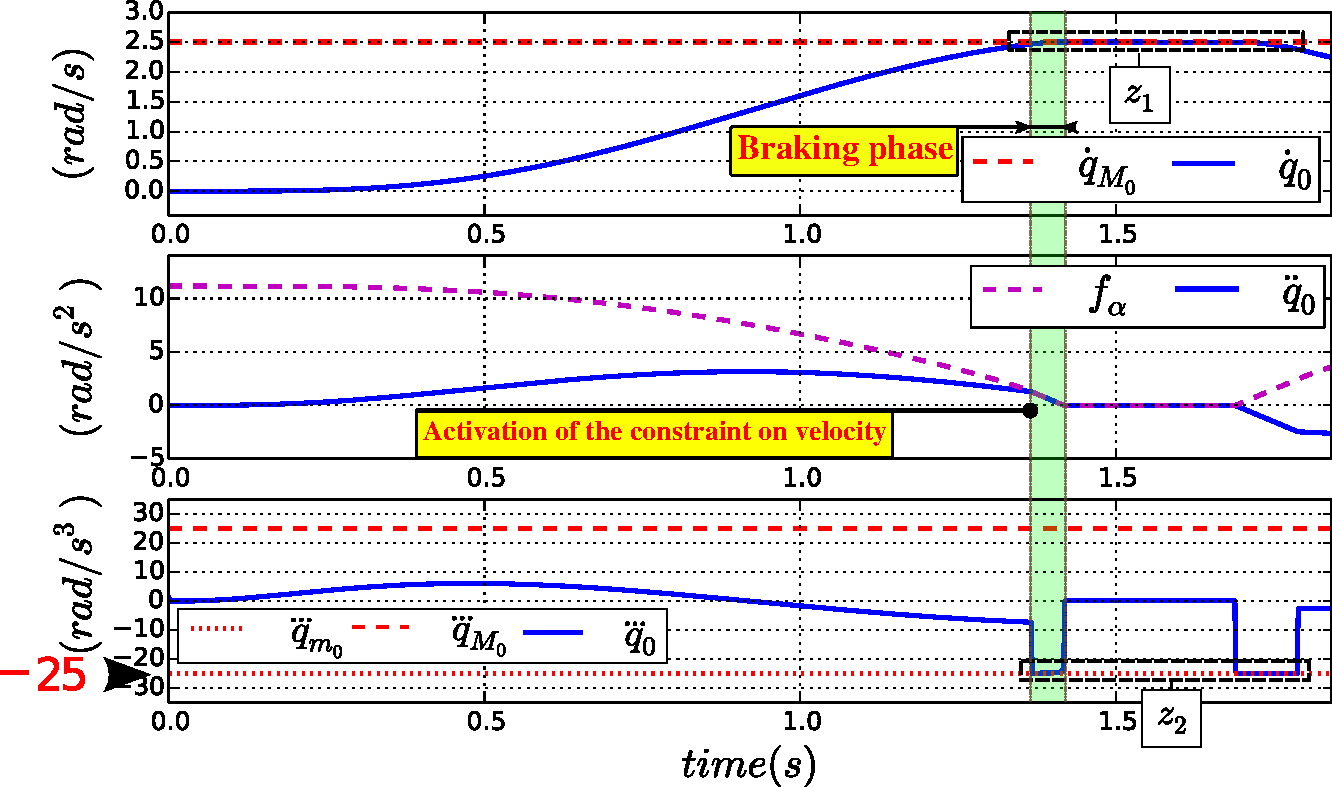
\includegraphics[width=0.99\columnwidth]{/home/anis/Desktop/THESIS_ANIS/THESIS/figures/Constrcomp/1_Vel_constr_jerk_comp_}
%\caption{State $S$ of joint $0$ during the braking phase to cope with a maximum velocity limit. In this test, the new constraint formulation (\ref{eq:q_ddot_vel_jerk_comp_aa_n1}) that takes into account the jerk capability $\dddot{q}_{M_{0}} = 25~rad.s^{-3}$ is used. Top to bottom: velocity, acceleration, jerk and $n_1$} 
%\label{fig:1_Vel_constr_jerk_comp_}
%\end{minipage}
%\hfill
%\begin{minipage}[c]{0.48\linewidth}
%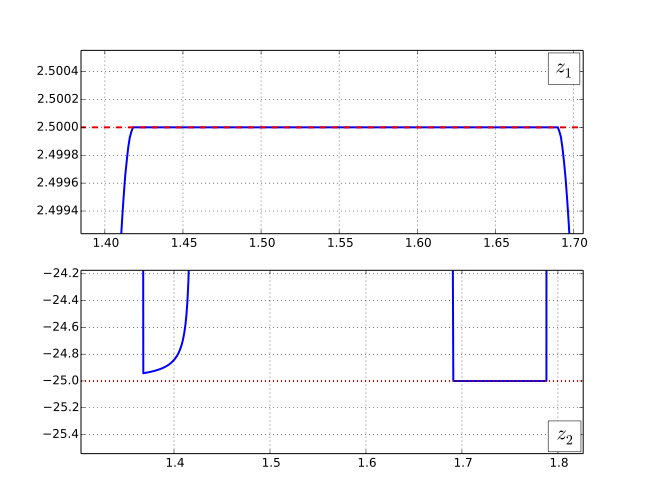
\includegraphics[width=0.99\columnwidth]{/home/anis/Desktop/THESIS_ANIS/THESIS/figures/Constrcomp/1_Vel_constr_jerk_comp_zoom}
%\caption{Zooms corresponding to Fig.~\ref{fig:1_Vel_constr_jerk_comp_}.} 
%\label{fig:1_Vel_constr_jerk_comp_zoom}
%\end{minipage}%
%\end{figure}
%\end{landscape}
%
%\begin{landscape}
%\begin{figure}
%\begin{minipage}[c]{0.48\linewidth}
%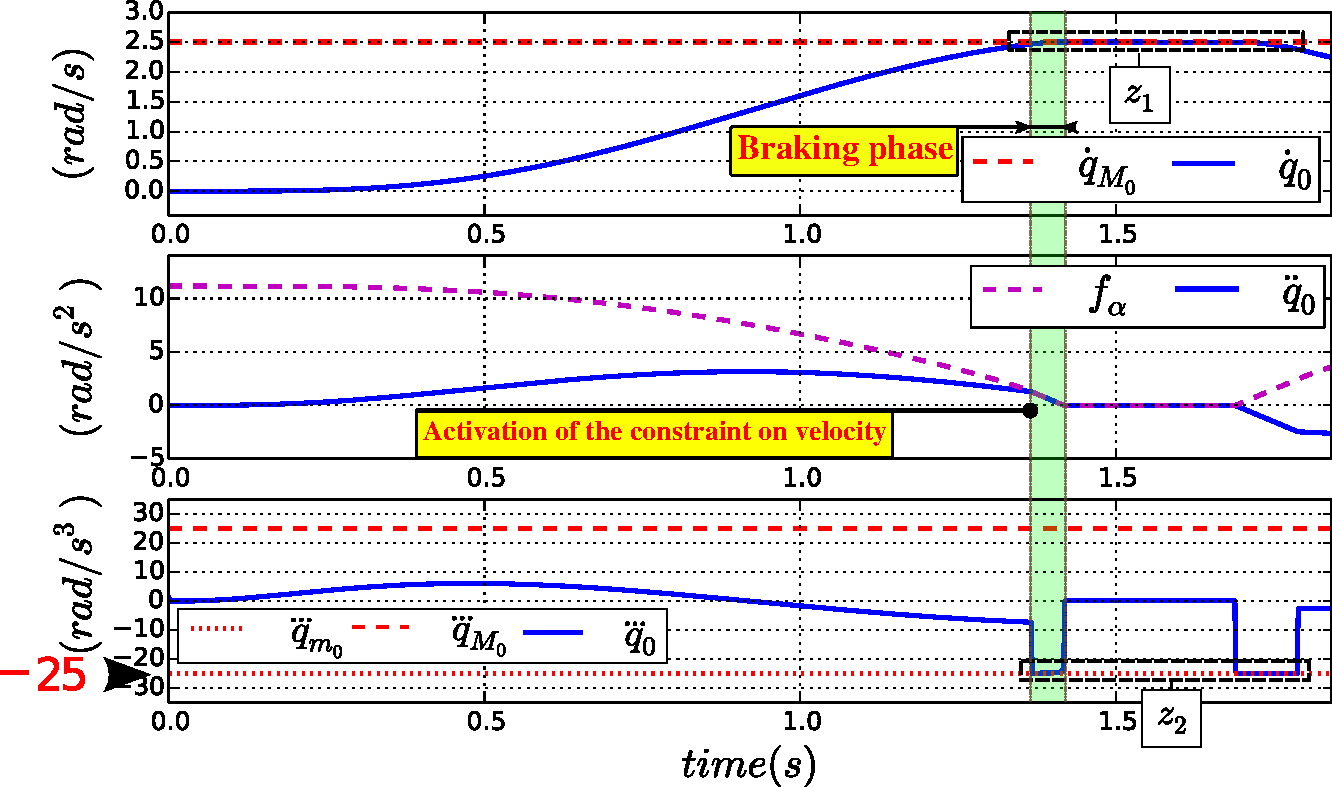
\includegraphics[width=0.99\columnwidth]{/home/anis/Desktop/THESIS_ANIS/THESIS/figures/Constrcomp/1_Vel_constr_jerk_comp_}
%\caption{State $S$ of joint $0$ during the braking phase to cope with a maximum velocity limit. In this test, the new constraint formulation (\ref{eq:q_ddot_vel_jerk_comp_aa_n1}) that takes into account the jerk capability $\dddot{q}_{M_{0}} = 25~rad.s^{-3}$ is used. Top to bottom: velocity, acceleration, jerk and $n_1$} 
%\label{fig:1_Vel_constr_jerk_comp_}
%\end{minipage}
%\hfill
%\begin{minipage}[c]{0.48\linewidth}
%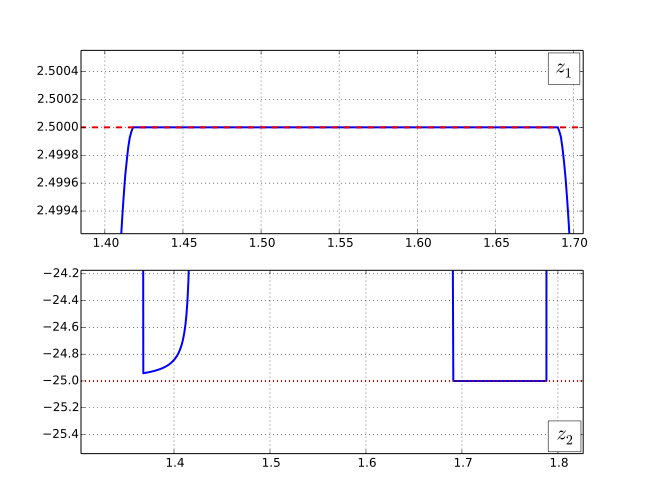
\includegraphics[width=0.99\columnwidth]{/home/anis/Desktop/THESIS_ANIS/THESIS/figures/Constrcomp/1_Vel_constr_jerk_comp_zoom}
%\caption{Zooms corresponding to Fig.~\ref{fig:1_Vel_constr_jerk_comp_}.} 
%\label{fig:1_Vel_constr_jerk_comp_zoom}
%\end{minipage}%
%\end{figure}
%\end{landscape}
%%%%%%%%%%%%%%%%%%%%%%%%%%SUBSECTION%%%%%%%%%%%%%%%%%%%%%%%%%%%%%
%%%%%%%%%%%%%%%%%%%%%%%%%%%%%%%%%%%%%%%%%%%%%%%%%%%%%%%%%%%%%%%%%
%%%%%%%%%%%%%%%%%%%%%%%%%%SUBSECTION%%%%%%%%%%%%%%%%%%%%%%%%%%%%%
\subsection{Joint position constraint incompatibility with deceleration and/or jerk limits}
\label{subsec:complete_b_ph}
With its \textit{naive}\footnote{Naive because it does not take into account the max/min amount of deceleration and jerk producible by the actuators of the robot.} formulation, the constraint on articular position (\ref{eq:cnt_lit_tme_step_1}) may become incompatible with the constraints on articular acceleration (\ref{eq:cnt_lit_tme_step_3}) and/or jerk (\ref{eq:cnt_lit_tme_step_4}) if a joint gets close to one of its position limits too fast (see Fig.~\ref{fig:Constraints_incompatibility_posi_constr1} and Fig.~\ref{fig:Constraints_incompatibility_posi_constr2}). In such case, \textit{admissible} deceleration and/or jerk may not be sufficient to allow a fast variation of the control torque, and it becomes impossible to bring both the articular acceleration and velocity to zero within only one control time-step. For example, the \labelText{{\color{red}\underline{complete}}}{label:complete} braking phase needed to be induced by an actuator to \textit{\textbf{properly}} cope with its upper position limit $q_M$ is as follows: 
\begin{enumerate}
\item at the activation of the constraint, the actuator starts jerking with maximum negative producible jerk $(\dddot{q} = \dddot{q}_m)$ (sub-phase \circled{1} in Fig.~\ref{fig:per_Pr_jerk_ala_3}). 
\item if the maximum producible deceleration $\ddot{q}_m$ is reached, braking jerk $\dddot{q}$ is brought to zero and the ``\textit{charged}'' deceleration $(\ddot{q} = \ddot{q}_m)$ is applied during several time-steps (sub-phase \circled{2} in Fig.~\ref{fig:per_Pr_jerk_ala_3}). 
\item the amount of deceleration in the joint is finally ``\textit{de-charged}'' and brought to zero by jerking positively with maximum producible jerk $(\dddot{q} = \dddot{q}_M)$ (sub-phase \circled{3} in Fig.~\ref{fig:per_Pr_jerk_ala_3}). By the end, the joint is stopped exactly at its upper position limit $q_M$. 
\end{enumerate}
\begin{figure}[!htbp]
{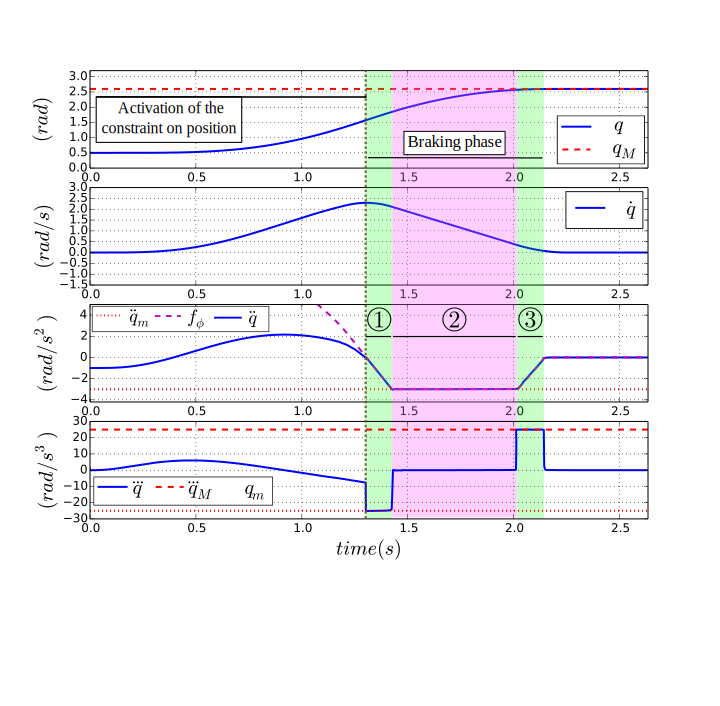
\includegraphics[width=1\columnwidth]{/home/anis/Desktop/THESIS_ANIS/THESIS/figures/Constrcomp/per_Posi_constr_jerk_acc_comp_complete_formula_3}}
\caption{Extended state $S$ of a joint during the induced \textit{complete} braking phase needed to \textit{\textbf{properly}} cope with an upper position limit $q_{M}$. The braking phase is composed of three sub-phases that each lasts for a number of time-steps: sub-phase~1 lasts $n_{15}$ control time-steps; sub-phase~2 lasts $n_{17}$ control time-steps and sub-phase~3 lasts $n_{19}$ control time-steps. Note that this illustration is not the result of a simulation. It represents the state of an actuator in case the \textit{complete} braking phase is used to cope with its upper position limit. Top to bottom: position, velocity, acceleration and jerk.} 
\label{fig:per_Pr_jerk_ala_3}
\end{figure}
As explained, coping with a joint position limit may fail because of incompatibilities with two other constraints: articular deceleration limits (\ref{eq:cnt_lit_3}) and producible articular jerk (\ref{eq:cnt_lit_4}). The resolution of these incompatibilities will be \textbf{methodically} performed as follows: 
\begin{enumerate}
\item \textbf{first}, independently from jerk capabilities, the naive expression of the position constraint (\ref{eq:cnt_lit_tme_step_1}) is modified to include solely the deceleration capabilities: $(\ddot{q}_m \leq 0)$ considering the upper position limit $(q_M \geq 0)$, and $(\ddot{q}_M  \geq 0)$ considering the lower position limit $(q_m \leq 0)$. With the new formulation, when coping for example with an upper articular position limit, the joint implicitly starts braking using its maximum deceleration capability $n_{3} \in \mathbb{N}$ iterations before reaching $q_M$ (see Fig.~\ref{fig:5_Posi_constr_acc_comp_312}). Using this formulation, both constraints on the articular position (\ref{eq:cnt_lit_1}) and the articular acceleration (\ref{eq:cnt_lit_3}) become compatible. The reflected bounds on the control variable $\ddot{q}_{|k}^{c}$ will be of the form: 
\begin{equation}
\begin{split}
f_{\xi}(q_m, \ddot{q}_M, n_4) \leq \ddot{q}_{|k}^{c} \leq f_{\gamma}(q_M, \ddot{q}_m, n_3). 
\label{eq:qddot_cond_to_satisfy_Acc_posi_compatibility}
\end{split}
\end{equation}
The proper methods to compute $n_3$, $n_4$, $f_{\gamma}$ and $f_{\xi}$ are fully defined in Section~\ref{subsec:case1}. 
\begin{figure}[!htbp]
{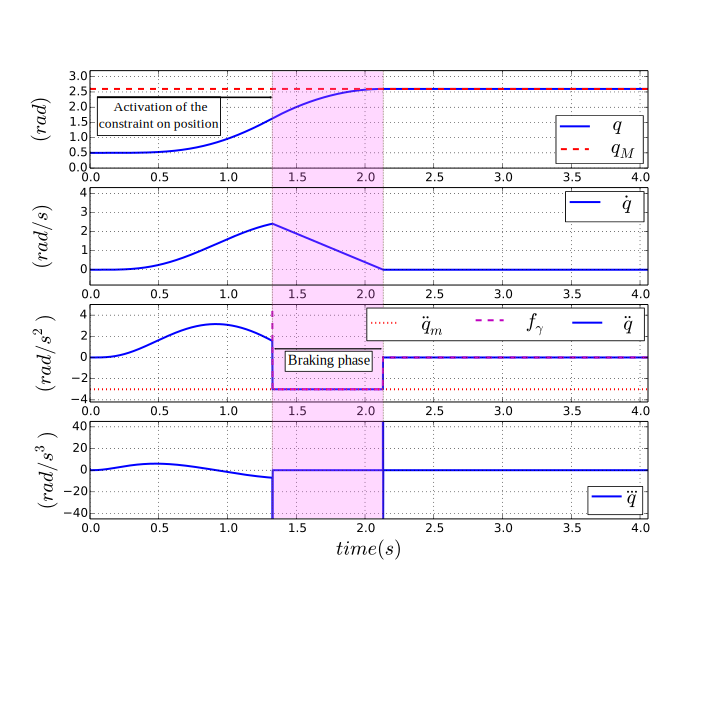
\includegraphics[width=1\columnwidth]{/home/anis/Desktop/THESIS_ANIS/THESIS/figures/Constrcomp/5_Posi_constr_acc_comp_312}}
\caption{Extended state $S$ of a joint during the induced braking phase needed to cope with an upper position limit $q_{M}$. Lasting $n_3$ control time-steps, the braking phase in this case takes into account only the articular deceleration capability $\ddot{q}_m$. Jerk limits are not considered. Top to bottom: position, velocity, acceleration and jerk.} 
\label{fig:5_Posi_constr_acc_comp_312}
\end{figure}
\item \textbf{Second}, independently from the articular deceleration capabilities, the naive expression of the constraint on articular position (\ref{eq:cnt_lit_tme_step_1}) is modified to include exclusively the actuator's jerk capabilities: $(\dddot{q}_m \leq 0)$ considering an upper position limit $(q_M \geq 0)$, and $(\dddot{q}_M \geq 0)$ when dealing with the lower position limit $(q_m \leq 0)$. With the resulting formulation, when coping for example with an upper position limit $q_M$, a braking movement is implicitly induced on the considered joint for a duration of $n_{5} \in \mathbb{N}$ control time-steps. Maximum producible negative jerk $\dddot{q}_m$ is applied by the actuator during this braking phase until the joint reaches and stops at upper position limit $q_{M}$. With such braking phase, both constraints on the articular position (\ref{eq:cnt_lit_1}) and jerk (\ref{eq:cnt_lit_3}) become compatible. In such case, the reflected bounds on the acceleration control variable will be of the form:
\begin{equation}
\begin{split}
f_{\theta}(q_m, \dddot{q}_M, n_6) \leq \ddot{q}_{|k}^{c} \leq f_{\eta}(q_M, \dddot{q}_m, n_5). 
\label{eq:qddot_cond_to_satisfy_Jerk_posi_compatibility}
\end{split}
\end{equation}
The proper methods to compute $n_5$, $n_6$, $f_{\eta}$ and $f_{\theta}$ are fully defined in Section~\ref{sec:secref2}. 
\item \textbf{Thirdly}, because of undesired oscillations (more details about this problem in subsection~\ref{sec:secref2}) that may appear in the movement of the constrained joint when using (\ref{eq:qddot_cond_to_satisfy_Jerk_posi_compatibility}) to cope with a position limit, this formulation is modified to include at the same time both the negative  $(\dddot{q}_m \leq 0)$ and positive $(\dddot{q}_M \geq 0)$ maximum producible articular jerk in both its left-hand and right-hand sides. When coping for example with an upper position limit, the  actuator should start braking with negative maximum producible jerk $\dddot{q}_m$ for $n_7$ control time-steps. As a consequence of this first braking sub-phase (phase \circled{1} in Fig.~\ref{fig:8_Podfgf12}), deceleration is ``\textit{loaded}'' in the articular joint. The actuator should then jerk positively with maximum producible jerk $\dddot{q}_M$ to bring the ``\textit{loaded}'' deceleration to zero (phase \circled{2} in Fig.~\ref{fig:8_Podfgf12}). The second sub-phase of the induced braking phase lasts for $n_9$ control time-steps and by its end, the actuator reaches and stops at its upper position limit $q_M$.  With such braking phase, the new formulation of the constraint on articular position will be of the form:
%Thirdly, because of oscillations\footnote{These oscillations are caused by not \textit{de-charging} the accumulated deceleration during the braking phase to cope with a position limit.} that may appear on the movement of the joint when using the previous formulation, (\ref{eq:qddot_cond_to_satisfy_Jerk_posi_compatibility}) will be modified to include positive and negative jerk capabilities as following:
\begin{equation}
\begin{split}
f_{\mu}(q_m, \dddot{q}_M, \dddot{q}_m, n_8, n_{10}) \leq \ddot{q}_{|k}^{c} \leq f_{\lambda}(q_M, \dddot{q}_m, \dddot{q}_M, n_7, n_9). 
\label{eq:qddot_cond_to_satisfy_Jerk_posi_compatibility_complete}
\end{split}
\end{equation}
The proper methods to compute $n_7$, $n_9$, $n_8$, $n_{10}$, $f_{\lambda}$ and $f_{\mu}$ are fully defined in Section~\ref{subsec:case3}. 
\begin{figure}[!htbp]
{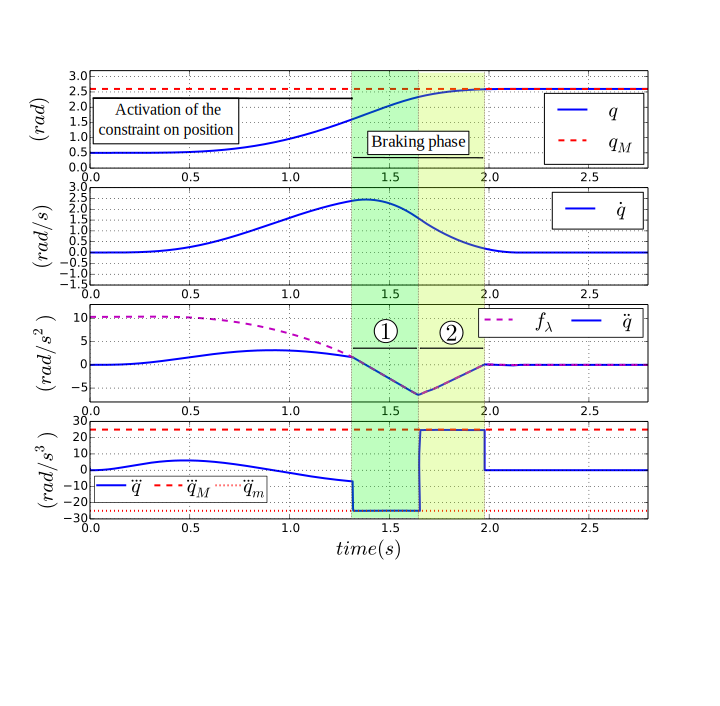
\includegraphics[width=1\columnwidth]{/home/anis/Desktop/THESIS_ANIS/THESIS/figures/Constrcomp/8_Podfgf12}}
\caption{Extended state $S$ of a joint during the induced braking phase needed to cope with an upper position limit $q_{M}$. The braking phase in this case is composed of two sub-phases: sub-phase~1 that lasts $n_{7}$ control time-steps and sub-phase~2 that lasts $n_{9}$ iterations. Note that, this illustration of the state of the joint is not the result of a simulation. It is a representation of how should be a braking phase induced using (\ref{eq:qddot_cond_to_satisfy_Jerk_posi_compatibility_complete}) when coping with an upper position limit. Top to bottom: position, velocity, acceleration and jerk.} 
\label{fig:8_Podfgf12}
\end{figure}
\item \textbf{Fourthly}, an expression of the constraint on articular position that takes into account at the same time both the jerk and deceleration capabilities is formulated. When included in the controller, this formulation renders the constraints on articular acceleration (\ref{eq:cnt_lit_3}) and jerk (\ref{eq:cnt_lit_4}) both compatible with the constraint on articular position (\ref{eq:cnt_lit_1}). Reflected bounds on the acceleration control variable $\ddot{q}_{|k}^{c}$ will be of the form: 
\begin{equation}
\begin{split}
f_{\rho}(q_m, \dddot{q}_M, \ddot{q}_M, n_{12}, n_{14}) \leq \ddot{q}_{|k}^{c} \leq f_{\pi}(q_M, \dddot{q}_m, \ddot{q}_m, n_{11}, n_{13}). 
\label{eq:qddot_cond_to_satisfy_Acc_Jerk_posi_compatibility}
\end{split}
\end{equation}
The proper methods to compute $n_{11}$, $n_{13}$, $n_{12}$, $n_{14}$, $f_{\pi}$ and $f_{\rho}$ are fully defined in Section~\ref{subsec:case4}. 
\item \textbf{Finally}, based on all the introduced forms of the various expressions proposed for the articular position constraint, a formulation that is based on the \nameref{label:complete} description of the braking phase used to \textit{\textbf{properly}} cope with a joint's upper/lower position limit is proposed. This includes the deceleration ``\textit{de-charging}'' sub-phase (sub-phase \circled{3} in Fig.~\ref{fig:per_Pr_jerk_ala_3}) that is necessary to prevent possible oscillations on the movement of the actuator during the activation of the constraint. This new and complete formulation takes into account both the negative and positive jerk capabilities $(\dddot{q}_m, \dddot{q}_M)$ together with the producible deceleration: $(\ddot{q}_m \leq 0)$ when coping with an upper position limit $(q_M \geq 0)$, and $(\ddot{q}_M \geq 0)$ when coping with a lower position limit $(q_m \leq 0)$. Without any drawbacks\footnote{No oscillations in the movement of the joint.}; both constraints on articular deceleration (\ref{eq:cnt_lit_3}) and jerk (\ref{eq:cnt_lit_4}) become compatible with the constraint on articular position (\ref{eq:cnt_lit_1}). With such formulation of the constraint on articular position derived from the \nameref{label:complete} description of the braking phase, the reflected bounds on the acceleration control variable are of the form: 
\begin{equation}
\begin{split}
f_{\chi}(q_m, \dddot{q}_M, \ddot{q}_M, \dddot{q}_m, n_{16}, n_{18}, n_{20}) \leq \ddot{q}_{|k}^{c} \leq f_{\phi}(q_M, \dddot{q}_m, \ddot{q}_m, \dddot{q}_M, n_{15}, n_{17}, n_{19}). 
\label{eq:qddot_cond_to_satisfy_Acc_Jerk_posi_compatibility2}
\end{split}
\end{equation}
The proper methods to compute $n_{15}$, $n_{17}$, $n_{19}$, $n_{16}$, $n_{18}$, $n_{20}$, $f_{\phi}$ and $f_{\chi}$ are fully defined in Section~\ref{subsec:case5}.
\end{enumerate}
\textbf{Note:} for a reactively controlled robot to optimally and \textit{properly} cope with a constraint on its articular position, considering both its max/min deceleration and jerk capabilities, the only formulation of the joint position constraint that should be implemented in its optimization control scheme is (\ref{eq:qddot_cond_to_satisfy_Acc_Jerk_posi_compatibility2}). The reader can directly check Section~\ref{subsec:case5} for the results on the behaviour of the robot when this formulation is used. The other formulations: (\ref{eq:qddot_cond_to_satisfy_Acc_posi_compatibility}), (\ref{eq:qddot_cond_to_satisfy_Jerk_posi_compatibility}), (\ref{eq:qddot_cond_to_satisfy_Jerk_posi_compatibility_complete}) and (\ref{eq:qddot_cond_to_satisfy_Acc_Jerk_posi_compatibility}), besides being presented for pedagogical reasons, their intermediary results are used for the formulation of (\ref{eq:qddot_cond_to_satisfy_Acc_Jerk_posi_compatibility2}) and taken individually, they can be used in specific cases where only the max/min producible articular deceleration OR jerk are of interest. Plus, due to the computation load linked to the $n_i$ parameters, these simpler formulations are faster to compute compared to the complete and proper formulation of the articular position constraint (\ref{eq:qddot_cond_to_satisfy_Acc_Jerk_posi_compatibility2}). \\

In the upcoming sections, the methods used to compute the introduced new formulations of the joint position constraint are furthermore detailed. In Section~\ref{sec:finalb}, the final bounds on the optimization control variable $\ddot{q}_{|k}^c$ that take into account the constraints on the articular position, velocity, acceleration and jerk all at the same time are formulated.
%%%%%%%%%%%%%%%%%%%%%%%%%%SUBSUBSECTION%%%%%%%%%%%%%%%%%%%%%%%%%%%%%
%%%%%%%%%%%%%%%%%%%%%%%%%%SUBSUBSECTION%%%%%%%%%%%%%%%%%%%%%%%%%%%%%
\subsubsection{Joint position constraint incompatibility with deceleration limits}
\label{subsec:case1}
In this section, the braking phase implicitly induced by a joint's actuator moving towards its upper position limit $q_{M}$ is considered. During this phase, the actuator's maximum producible deceleration is $\ddot{q}_{m}$. Its jerk capabilities $[\dddot{q}_{m}, \dddot{q}_{M}]$ are not considered. The extended state of the system during such braking phase, that makes the actuator stop at its position limit $q_{M}$, can be described as:
\begin{equation} 
\begin{split}
\textit{S}_{|k+1}&\left\{\begin{array}{lcl}
q_{|k+1} \hspace{1mm}= q_{|k} + \dot{q}_{|k} \delta t, \\
\dot{q}_{|k+1} \hspace{1mm}= \dot{q}_{|k} + \ddot{q}_{m} \delta t;
\end{array}\right.\\
\textit{S}_{|k+2}&\left\{\begin{array}{lcl}
q_{|k+2} \hspace{1mm}= q_{|k+1} + \dot{q}_{|k+1} \delta t, \\
\dot{q}_{|k+2} \hspace{1mm}= \dot{q}_{|k+1} + \ddot{q}_{m} \delta t;
\end{array}\right.\\
&\hspace{7mm}\vdots\ \hspace{12mm}\vdots\ \\
\textit{S}_{|k+n_{3}}&\left\{\begin{array}{lcl}
q_{|k+n_{3}} = q_{|k+n_{3}-1} + \dot{q}_{|k+n_{3}-1} \delta t, \\
\dot{q}_{|k+n_{3}} = \dot{q}_{|k+n_{3}-1} + \ddot{q}_{m} \delta t.
\end{array}\right.
\end{split}
\label{eq:discretized_dynamics_posi_decel}
\end{equation}
With: $q_{|k} \geq 0$, $\dot{q}_{|k} \geq 0$ and  $\ddot{q}_{m} \leq 0$ (braking phase). The joint position evolution in $n_3  \geq 1$ iterations is equal to the general form\footnote{Computed using Maple \cite{maple}.} of the numerical sequence (\ref{eq:discretized_dynamics_posi_decel}):
\begin{equation}
\begin{split}
q_{|k+n_3} = q_{|k} + n_3 \dot{q}_{|k} \delta t + \frac{(n_3^2-n_3)}{2} \ddot{q}_{m} \delta t^2.
\label{eq:q_evolution_with_const_qddot_m}
\end{split}
\end{equation}
The condition $q_{|k+n_3} \leq q_{M}$ for all integer $n_3$ leads to:
\begin{equation}
\begin{split}
\dot{q}_{|k}^{c} \leq \underbrace{\frac{(q_M-q_{|k})}{n_3 \delta t} - \frac{(n_3-1)}{2} \ddot{q}_m \delta t}_{f_{{\gamma}_{vel}}}. 
\label{eq:q_dot_posi_acc_comp}
\end{split}
\end{equation}
With $\dot{q}_{|k}^{c}$: the velocity control input in case the robot is controlled at the kinematic-level. The equivalent constraint on the acceleration control variable $\ddot{q}_{|k}^{c}$, in case the robot is controlled at the dynamic-level, that generates the same braking profile can be written:
\begin{equation}
\begin{split}
\ddot{q}_{|k}^{c} \leq \frac{(q_M-q_{|k})}{n_3 \delta t^2} - \frac{\dot{q}_{|k}}{\delta t} - \frac{(n_3-1)}{2} \ddot{q}_m.
\label{eq:q_ddot_posi_acc_comp_upp}
\end{split}
\end{equation}
With: 
\begin{equation}
\begin{split}
n_3 = \frac{-\sqrt{-2 \ddot{q}_m (q_M - q_{|k})}}{\ddot{q}_m \delta t},
\label{eq:n_3_Acc_posi_comp}
\end{split}
\end{equation}
the integer minimizing the right-hand side of (\ref{eq:q_ddot_posi_acc_comp_upp}). \\
The transition from (\ref{eq:q_dot_posi_acc_comp}) to (\ref{eq:q_ddot_posi_acc_comp_upp}) can easily be proven as follows: in case of a velocity control input $\vect{\dot{q}}_{|k}^{c}$, the resulting articular velocity at the next time-step $k+1$ is: $\vect{\dot{q}}_{|k+1} (output)= \vect{\dot{q}}_{|k}^{c} (input)$. On the other hand, in case of a control at the dynamic-level: $\vect{\dot{q}}_{|k+1} = \vect{\dot{q}}_{|k}+\vect{\ddot{q}}_{|k}^{c}\delta t$, with  $\vect{\ddot{q}}_{|k}^{c}$: the control variable linked to the control torque input $\vect{\tau}_{|k}^{c}$ and $\vect{\dot{q}}_{|k+1}$ the resulting  articular velocity. The relation between the kinematic-level and the dynamic-level control inputs that results into the same articular movement can then be derived: $\vect{\dot{q}}_{|k}+\vect{\ddot{q}}_{|k}^{c}\delta t = \vect{\dot{q}}_{|k}^{c}$.\\

Following the same reasoning for the lower articular position limit, when reflected on the acceleration control variable, the condition $q_{|k+n_4} \geq q_{m}$ for all integer $n_4 \geq 1$ leads to:
\begin{equation}
\begin{split}
\ddot{q}_{|k}^{c} \geq \frac{(q_m-q_{|k})}{n_4 \delta t^2} - \frac{\dot{q}_{|k}}{\delta t} - \frac{(n_4-1)}{2} \ddot{q}_M. 
\label{eq:q_ddot_posi_acc_comp_low}
\end{split}
\end{equation}
With: 
\begin{equation}
\begin{split}
n_4 = \frac{\sqrt{-2 \ddot{q}_M (q_m - q_{|k})}}{\ddot{q}_M \delta t},
\label{eq:n_4_Acc_posi_comp}
\end{split}
\end{equation}
maximizing the right-hand side of (\ref{eq:q_ddot_posi_acc_comp_low}). We recall that: $n_3$ is the number of control time-steps corresponding to the duration of a braking phase implicitly induced by an actuator moving towards its upper position limit $q_M$, and during which both its acceleration and velocity are brought to zero by decelerating with maximum negative producible acceleration $\ddot{q}_m$; and $n_4$ is the number of control time-steps corresponding to the duration of a braking phase implicitly induced by an actuator moving towards its lower position limit $q_m$, and during which both its acceleration and velocity are brought to zero by accelerating positively with maximum producible acceleration $\ddot{q}_M$. \\
$\textit{f}_{\xi}$ and $\textit{f}_{\gamma}$ are respectively equivalent to the right-hand sides of (\ref{eq:q_ddot_posi_acc_comp_low}) and (\ref{eq:q_ddot_posi_acc_comp_upp}).
%********************************************************************%
\paragraph{Illustration 2}
For this simulation, using the test case scenario, the controller is implemented with the new formulation of the constraint on articular position (\ref{eq:q_ddot_posi_acc_comp_upp}), that takes into account the available deceleration capability $(\ddot{q}_{m_{0}} = -100~rad.s^{-2})$. In this case, just like the test case scenario, joint $0$ moves towards its maximum allowed position $q_{M_{0}}$. 

Fig.~\ref{fig:4_Posi_constr_acc_comp_100} shows the extended state of joint $0$ as an implicitly induced braking phase is started at the right time and during which the actuator uses its maximum producible deceleration $\ddot{q}_{m_{0}}$ to cope with its upper position limit $q_{M_{0}}$. As the articular jerk limits $[\dddot{q}_{m_{0}}, \dddot{q}_{M_{0}}]$ are not considered in this formulation of the constraint on articular position, a jerk peak is induced at the beginning of the braking phase at the activation of the constraint. When this new formulation of the articular position constraint is used, including the naive acceleration/deceleration constraint (\ref{eq:cnt_lit_tme_step_3}) in the configuration of the controller will not result into an infeasible control problem. The incompatibility between the articular position and articular deceleration constraint is resolved. \\
On the other hand, it has been impossible to cope with the same upper position limit using the naive formulation of the constraint on articular position (\ref{eq:cnt_lit_tme_step_1}). Much larger deceleration capabilities (\ref{eq:cnt_lit_tme_step_3}) are needed for a braking phase that is induced only one time-step before joint $0$ reaches $q_{M_{0}}$. \\
Fig.~\ref{fig:5_Posi_constr_acc_comp_3} illustrates how the starting time of the braking phase is automatically adapted to the amount of available deceleration. For example, when  $\ddot{q}_{m_{0}}$ is reduced to $-3~rad.s^{-2}$, the braking phase starts earlier and lasts longer.
%%4
%\begin{figure}[!htbp]
%\centering
%{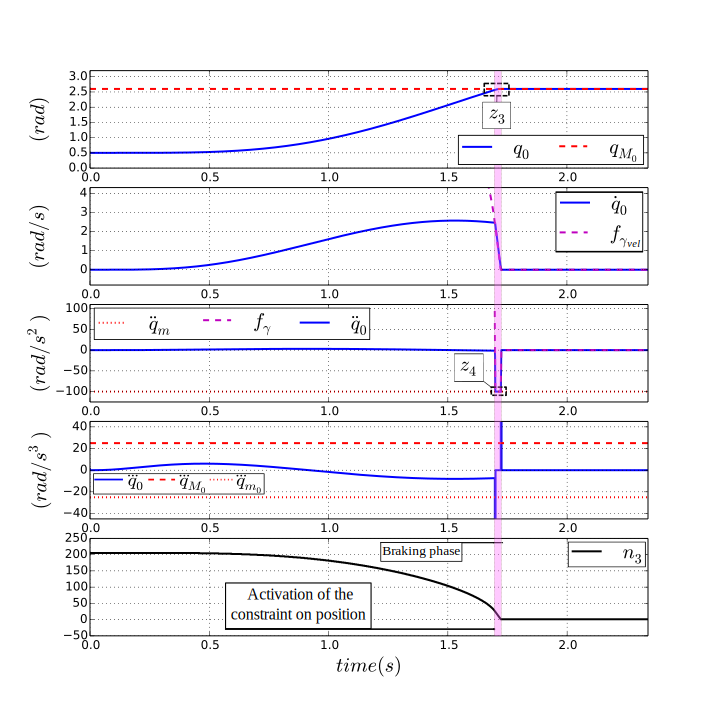
\includegraphics[width=0.8\columnwidth]{/home/anis/Desktop/THESIS_ANIS/THESIS/figures/Constrcomp/4_Posi_constr_acc_comp_100}}
%\caption{State $S$ of joint $0$ during the braking phase to cope with a maximum position limit $\q_{M_{0}}$; The new constraint formulation (\ref{eq:q_ddot_posi_acc_comp_upp}) that takes into account the deceleration capability $\ddot{q}_{m_{0}} = -100~rad.s^{-2}$ is used. Top to bottom: position, velocity, acceleration, jerk and $n_3$} 
%\label{fig:4_Posi_constr_acc_comp_100}
%\end{figure}
%%5
%\begin{figure}[!htbp]
%\centering
%{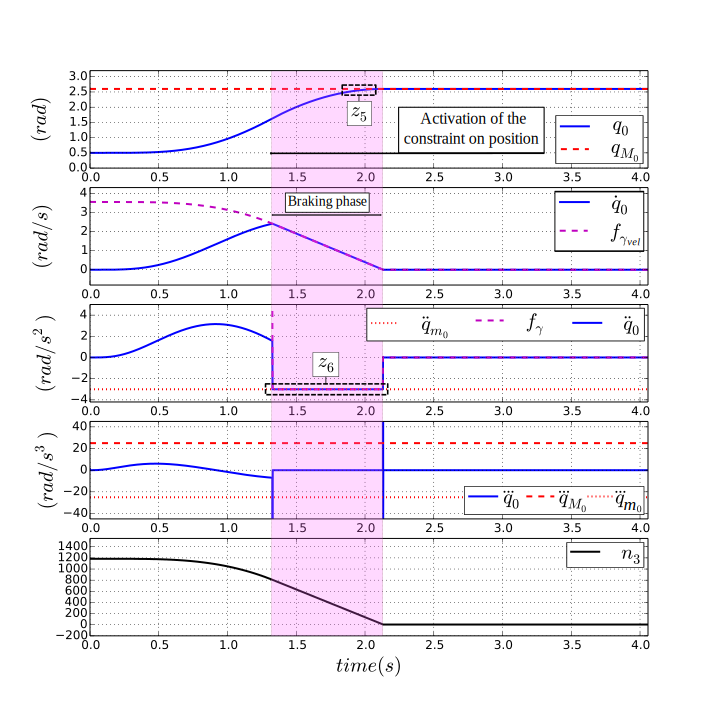
\includegraphics[width=0.8\columnwidth]{/home/anis/Desktop/THESIS_ANIS/THESIS/figures/Constrcomp/5_Posi_constr_acc_comp_3}}
%\caption{State $S$ of joint $0$ during the braking phase to cope with a maximum position limit; The new constraint formulation (\ref{eq:q_ddot_posi_acc_comp_upp}) that takes into account the deceleration capability $\ddot{q}_{m_{0}} = -3~rad.s^{-2}$ is used. Top to bottom: position, velocity, acceleration, jerk and $n_3$.} 
%\label{fig:5_Posi_constr_acc_comp_3}
%\end{figure}
%\begin{figure}[!htbp]
%\centering
%{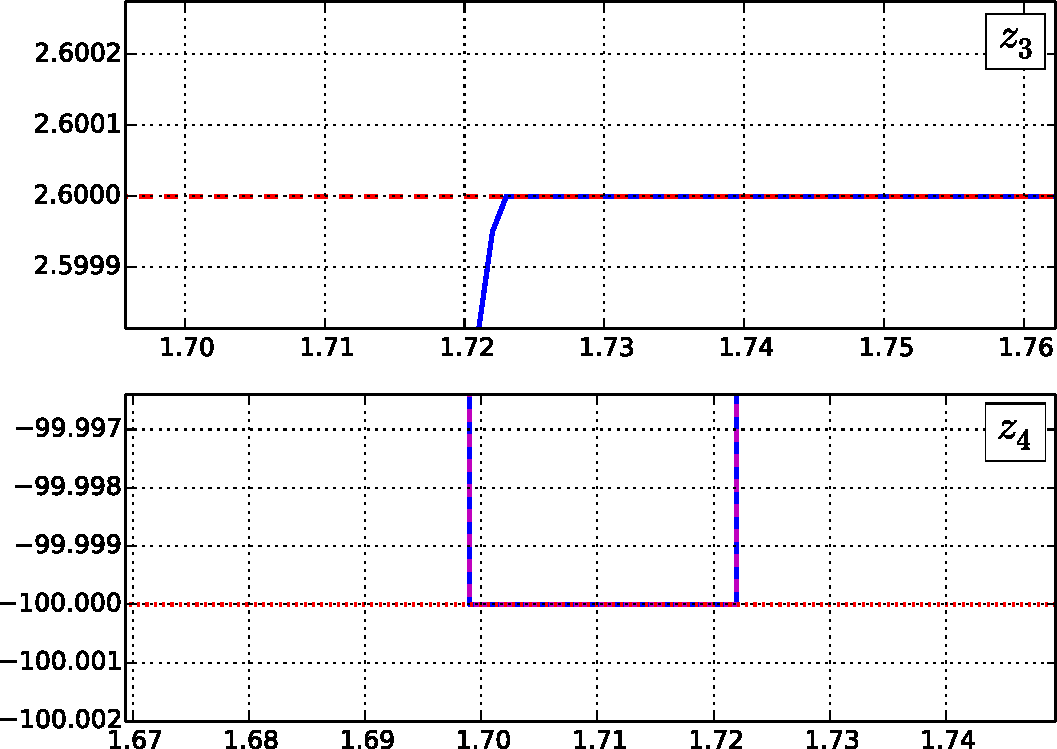
\includegraphics[width=0.8\columnwidth]{/home/anis/Desktop/THESIS_ANIS/THESIS/figures/Constrcomp/4_Posi_constr_acc_comp_100_zoom}}
%\caption{Zooms corresponding to Fig.~\ref{fig:4_Posi_constr_acc_comp_100}.} 
%\label{fig:4_Posi_constr_acc_comp_100_zoom}
%\end{figure}
%\begin{figure}[!htbp]
%\centering
%{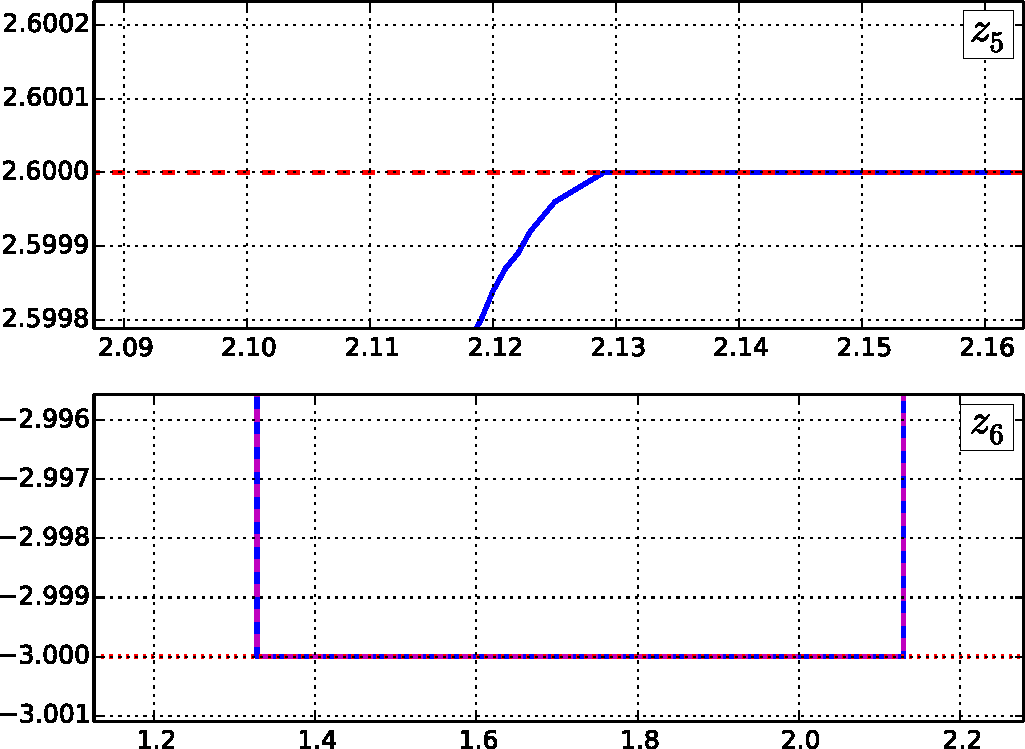
\includegraphics[width=0.8\columnwidth]{/home/anis/Desktop/THESIS_ANIS/THESIS/figures/Constrcomp/5_Posi_constr_acc_comp_3_zoom}}
%\caption{Zooms corresponding to Fig.~\ref{fig:5_Posi_constr_acc_comp_3}.} 
%\label{fig:5_Posi_constr_acc_comp_3_zoom}
%\end{figure}
\begin{landscape}
\begin{figure}
\begin{minipage}[c]{0.5\linewidth}
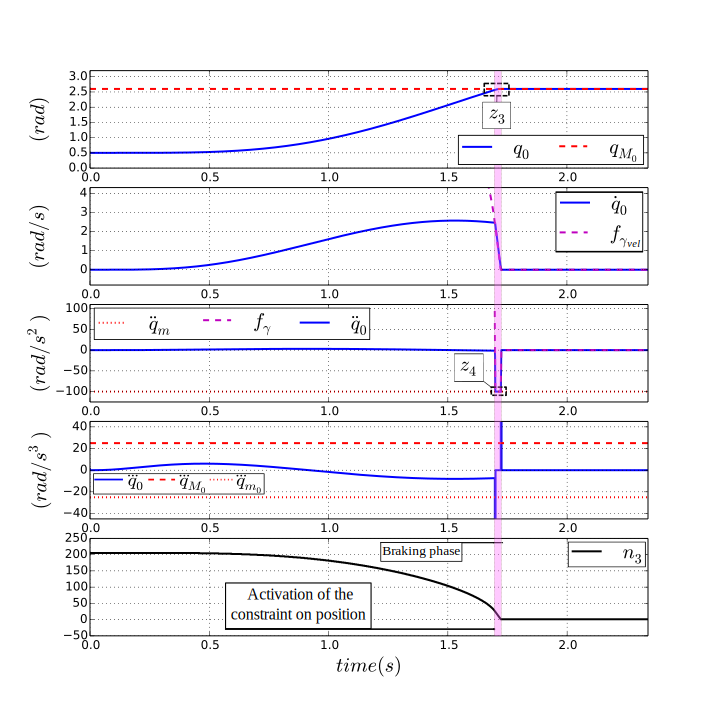
\includegraphics[width=0.99\columnwidth]{/home/anis/Desktop/THESIS_ANIS/THESIS/figures/Constrcomp/4_Posi_constr_acc_comp_100}
\caption{Extended state $S$ of joint $0$ during the braking phase implicitly induced by the joint's actuator to cope with the upper position limit $q_{M_{0}}$. The new formulation of the constraint on articular position (\ref{eq:q_ddot_posi_acc_comp_upp}) that takes into account the deceleration capability $\ddot{q}_{m_{0}} = -100~rad.s^{-2}$ is used. Top to bottom: position, velocity, acceleration, jerk and $n_3$. See $z_3$ and $z_4$ in Fig.~\ref{fig:4_Posi_constr_acc_comp_100_zoom}}.} 
\label{fig:4_Posi_constr_acc_comp_100}
\end{minipage}
\hfill
\begin{minipage}[c]{0.5\linewidth}
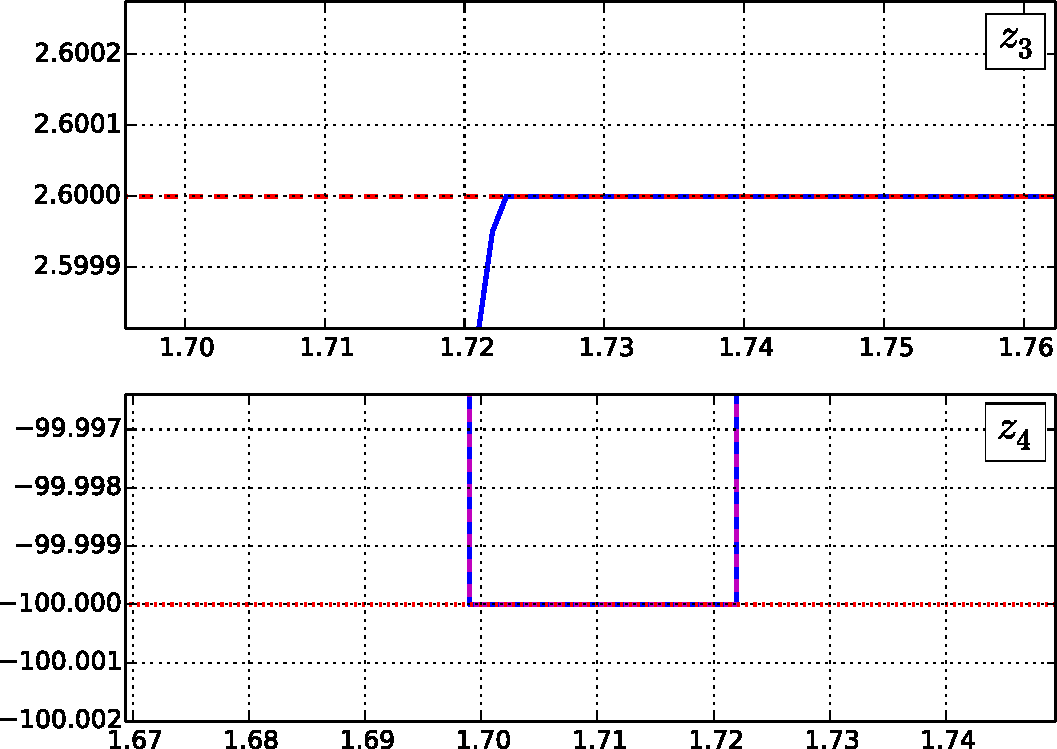
\includegraphics[width=0.90\columnwidth]{/home/anis/Desktop/THESIS_ANIS/THESIS/figures/Constrcomp/4_Posi_constr_acc_comp_100_zoom}
\caption{Zooms corresponding to Fig.~\ref{fig:4_Posi_constr_acc_comp_100}.} 
\label{fig:4_Posi_constr_acc_comp_100_zoom}
\end{minipage}%
\end{figure}
\end{landscape}
\begin{landscape}
\begin{figure}
\begin{minipage}[c]{0.5\linewidth}
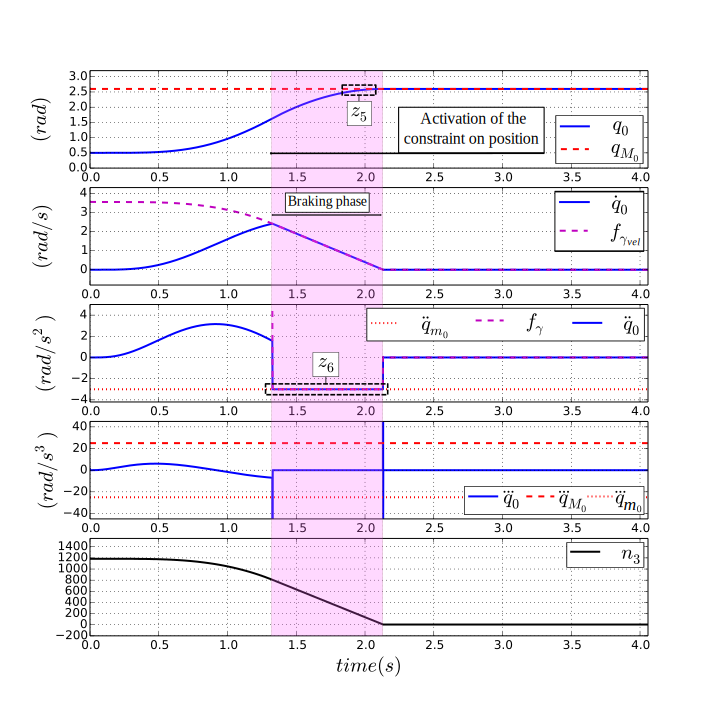
\includegraphics[width=0.99\columnwidth]{/home/anis/Desktop/THESIS_ANIS/THESIS/figures/Constrcomp/5_Posi_constr_acc_comp_3}
\caption{Extended state $S$ of joint $0$ during the braking phase implicitly induced by the joint's actuator to cope with the upper position limit $q_{M_{0}}$. The new formulation of the constraint on articular position (\ref{eq:q_ddot_posi_acc_comp_upp}) that takes into account the deceleration capability $\ddot{q}_{m_{0}} = -3~rad.s^{-2}$ is used. Top to bottom: position, velocity, acceleration, jerk and $n_3$. See $z_5$ and $z_6$ in Fig.~\ref{fig:5_Posi_constr_acc_comp_3_zoom}}.} 
\label{fig:5_Posi_constr_acc_comp_3}
\end{minipage}
\hfill
\begin{minipage}[c]{0.5\linewidth}
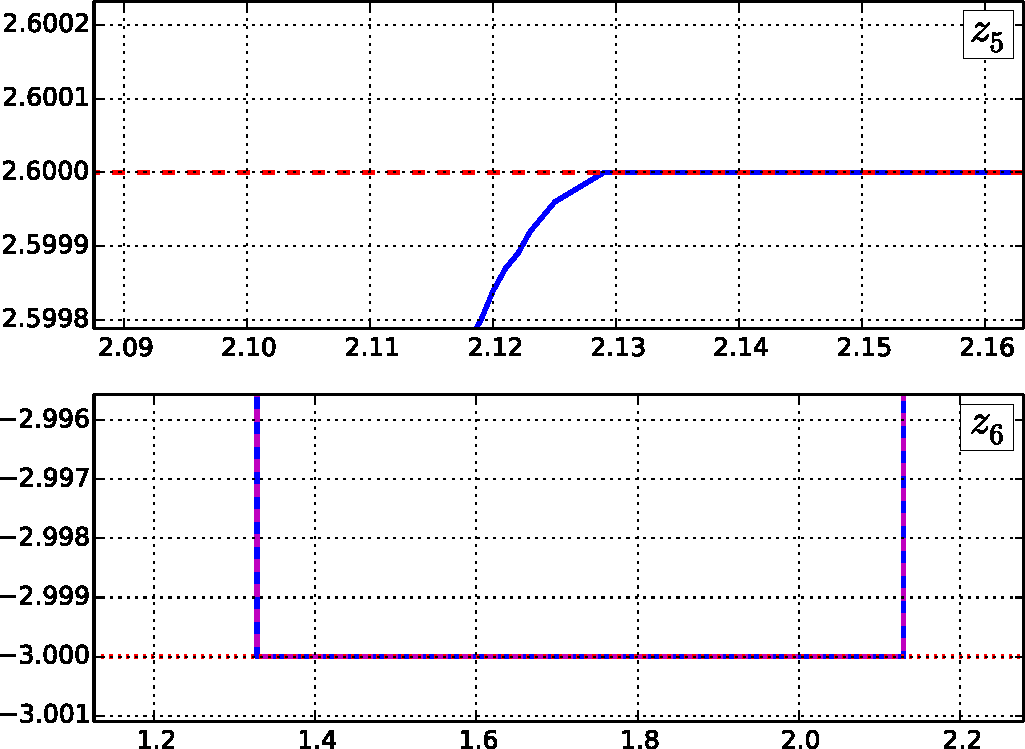
\includegraphics[width=0.90\columnwidth]{/home/anis/Desktop/THESIS_ANIS/THESIS/figures/Constrcomp/5_Posi_constr_acc_comp_3_zoom}
\caption{Zooms corresponding to Fig.~\ref{fig:5_Posi_constr_acc_comp_3}.} 
\label{fig:5_Posi_constr_acc_comp_3_zoom}
\end{minipage}%
\end{figure}
\end{landscape}
%%%%%%%%%%%%%%%%%%%%%%%%%%SUBSUBSECTION%%%%%%%%%%%%%%%%%%%%%%%%%%%%%
%%%%%%%%%%%%%%%%%%%%%%%%%%SUBSUBSECTION%%%%%%%%%%%%%%%%%%%%%%%%%%%%%
\subsubsection{Joint position constraint incompatibility with jerk limits 1}
\label{sec:secref2}
We consider a braking phase for a joint moving towards its upper position limit $q_M$. In this case, only the lower limit $\dddot{q}_m$ of jerk capabilities is considered. Maximum producible deceleration $\ddot{q}_m$ is not taken into account. The extended state \textit{S} of the system during this implicitly induced braking phase, that makes the joint's actuator stop at its upper position limit $q_M$, can be described as: 
\begin{equation} 
\begin{split}
\textit{S}_{|k+1}&\left\{\begin{array}{lcl}
q_{|k+1} \hspace{2mm}= q_{|k} + \dot{q}_{|k} \delta t, \\
\dot{q}_{|k+1} \hspace{2mm}= \dot{q}_{|k} + \ddot{q} \delta t, \\
\ddot{q}_{|k+1} \hspace{2mm}= \ddot{q}_{|k} + \dddot{q}_{m} \delta t;
\end{array}\right.\\
\textit{S}_{|k+2}&\left\{\begin{array}{lcl}
q_{|k+2} \hspace{2mm}= q_{|k+1} + \dot{q}_{|k+1} \delta t, \\
\dot{q}_{|k+2} \hspace{2mm}= \dot{q}_{|k+1} + \ddot{q}_{|k+1} \delta t, \\
\ddot{q}_{|k+2} \hspace{2mm}= \ddot{q}_{|k+1} + \dddot{q}_{m} \delta t;
\end{array}\right.\\
& \hspace{7mm}\vdots\ \hspace{13mm}\vdots\ \\
\textit{S}_{|k+n_{5}}&\left\{\begin{array}{lcl}
q_{|k+n_{5}} = q_{|k+n_{5}-1} + \dot{q}_{|k+n_{5}-1} \delta t, \\
\dot{q}_{|k+n_{5}} = \dot{q}_{|k+n_{5}-1} + \ddot{q}_{|k+n_{5}-1} \delta t, \\
\ddot{q}_{|k+n_{5}} = \ddot{q}_{|k+n_{5}-1} + \dddot{q}_{m} \delta t.
\end{array}\right.
\end{split}
\label{eq:discretized_dynamics_posi_jerk_braking}
\end{equation}
With: $q_{|k} \geq 0$, $\dot{q}_{|k} \geq 0$ and  $\dddot{q}_{m} \leq 0$. The joint position evolution within $n_5$ iterations is equal to the general form\footnote{Computed using Maple \cite{maple}.} of the numerical sequence (\ref{eq:discretized_dynamics_posi_jerk_braking}):
\begin{equation}
q_{|k+n_5} = q_{|k} + n_5 \dot{q}_{|k} \delta t +  \frac{\left(n_5^2-n_5\right)}{2} \ddot{q}_{|k} \delta t^2 + \left(\frac{n_5^3}{6}-\frac{n_5^2}{2}+\frac{n_5}{3}\right) \dddot{q}_m \delta t^3.
\label{eq:q_evolution_with_const_qdddot_m}
\end{equation}
The condition $q_{|k+n_5} \leq q_{M}$ for all integer $n_5$ leads to:
\begin{equation}
\begin{split}
\ddot{q}_{|k}^{c} \leq \frac{2\left(q_M-q_{|k}\right)}{\left(n_5^2-n_5\right) \delta t^2} - \frac{2 \dot{q}_{|k}}{\left(n_5-1\right) \delta t} - \frac{\left(\frac{n_5^2}{3}-n_5+\frac{2}{3}\right)}{\left(n_5-1\right)}\dddot{q}_m \delta t,
\label{eq:q_ddot_posi_jerk_comp_upp}
\end{split}
\end{equation}
with $n_5$, the integer minimizing the right-hand side of (\ref{eq:q_ddot_posi_jerk_comp_upp}). It can be computed analytically. By differentiating this expression w.r.t $n_5$:
\begin{equation}
\left\{\begin{array}{lcl}
n_5 \geq 3, \\
\begin{split}
-&\left(\frac{1}{3} \dddot{q}_m \delta t^3\right) n_5^4 + \left(\frac{2}{3} \dddot{q}_{|m} \delta t^3\right) n_5^3  \\
+&\left(2 \dot{q}_{|k} \delta t - \frac{1}{3} \dddot{q}_m \delta t^3\right) n_5^2 \\
+& 4 \left(q_M-q_{|k}\right) n_5 - 2\left(q_M-q_{|k}\right)=0.
\end{split}
\end{array}\right.
\label{eq:n_5_eq_new}
\end{equation}
$n_5$ is the rounded-up real root of (\ref{eq:n_5_eq_new}). It must be $\geq 3$ so that $\dddot{q}_m$ is always part of (\ref{eq:q_ddot_posi_jerk_comp_upp})\\
Following the same reasoning for the lower position limit, the condition $q_{|k+n_6} \geq q_{m}$ for all integer $n_6 \geq 3$ can be reflected on the acceleration control variable as:
\begin{equation}
\begin{split}
\ddot{q}_{|k}^{c}  \geq \frac{2(q_m - q_{|k})}{\left(n_6^2 - n_6\right)\delta t^2} - \frac{2 \dot{q}_{|k}}{(n_6-1)\delta t} 
- \frac{\left(\frac{n_6^2}{3} - n_6 + \frac{2}{3}\right)}{(n_6-1)}\dddot{q}_M \delta t
\label{eq:q_ddot_posi_jerk_comp_low}
\end{split}
\end{equation}
With: 
\begin{equation}
\left\{\begin{array}{lcl}
n_6 \geq 3, \\
\begin{split}
-&\left(\frac{1}{3} \dddot{q}_M \delta t^3\right) n_6^4 + \left(\frac{2}{3} \dddot{q}_{|M} \delta t^3\right) n_6^3  \\
+&\left(2 \dot{q}_{|k} \delta t - \frac{1}{3} \dddot{q}_M \delta t^3\right) n_6^2 \\
+& 4 \left(q_m-q_{|k}) n_6 - 2(q_m-q_{|k}\right)=0.
\end{split}
\end{array}\right.
\label{eq:n_6_eq_new}
\end{equation}
$n_6$ is the rounded up real root of (\ref{eq:n_6_eq_new}) that maximizes the right-hand side of (\ref{eq:q_ddot_posi_jerk_comp_low}). We recall that: $n_5$ is the number of control time-steps corresponding to the duration of a braking phase implicitly induced by an actuator moving towards its upper position limit $q_M$, and during which both its acceleration and velocity are brought to zero by jerking with maximum negative producible jerk $\dddot{q}_m$ and; $n_6$ is the number of control time-steps corresponding to the duration of a braking phase implicitly induced by an actuator moving towards its lower position limit $q_m$, and during which both its acceleration and velocity are brought to zero by jerking with maximum positive producible jerk $\dddot{q}_M$. \\
$\textit{f}_{\theta}$ and $\textit{f}_{\eta}$ are respectively equivalent to the right-hand sides of (\ref{eq:q_ddot_posi_jerk_comp_low}) and (\ref{eq:q_ddot_posi_jerk_comp_upp}). \\
\noindent\begin{minipage}{\textwidth}
\renewcommand\footnoterule{}                  %% This line should come here.
\begin{algorithm}[H]
\caption{Compute $n_{5}, n_{6}, f_{\theta}$ and $f_{\eta}$}
\label{alg:compute_f_theta_f_eta_n_5_n_6}
\begin{algorithmic}[1]
%f_{\theta}(n_{6})     f_{\eta}(n_{5})
%    n1_pos         n1_neg 
\Require $q_M, q_m, q_{|k}, \dot{q}_{|k},\dddot{q}_{M},\dddot{q}_{m}, \delta t$
\myState{$f_{{\theta}_{max}} \gets \ddot{q}_{m}$} \Comment{temporary lower bound of $\ddot{q}_{|k}^{c}$}
\myState{$f_{{\eta}_{min}} \gets \ddot{q}_{M}$} \Comment{temporary upper bound of $\ddot{q}_{|k}^{c}$}
\For{($i = 3 \rightarrow N$)}
        \myState{$n_{5}^{*} \gets i \qquad n_{6}^{*} \gets i$}
        \myState{$f_{\theta}^{*} \gets f_{\theta}(q_m, \dddot{q}_M, q_{|k}, \dot{q}_{|k}, \dddot{q}_M, n_{6}^{*})$} 
        \myState{$f_{\eta}^{*} \gets f_{\eta}(q_M, \dddot{q}_m, q_{|k}, \dot{q}_{|k}, \dddot{q}_m, n_{5}^{*})$}
        \If{($f_{\theta}^{*} \geq f_{{\theta}_{max}}$)}
            \State{$f_{{\theta}_{max}} \gets f_{\theta}^{*} \qquad n_{6} \gets n_{6}^{*} $}
        \EndIf   
        \If{($f_{\eta}^{*} \leq f_{{\eta}_{min}}$)}
            \State{$f_{{\eta}_{min}} \gets f_{\eta}^{*} \qquad n_{5} \gets n_{5}^{*}$}
        \EndIf            
\EndFor
\State{$f_{\theta} \gets f_{{\theta}_{max}} \qquad f_{\eta} \gets f_{{\eta}_{min}}$}
\myState \Return{$n_{5}, n_{6}, f_{\theta}, f_{\eta}$}\;
\end{algorithmic}
\end{algorithm}
\end{minipage} \\
\\
Finally, $n_{5}, n_{6}, f_{\theta}$ and $f_{\eta}$ can be computed numerically as shown by Algorithm~\ref{alg:compute_f_theta_f_eta_n_5_n_6}. 
N in Algorithm~\ref{alg:compute_f_theta_f_eta_n_5_n_6} can be fixed heuristically, it must be however $\geq$ to the solutions of (\ref{eq:n_5_eq_new}) and (\ref{eq:n_6_eq_new}). More details on how to compute this parameter in Section~\ref{sec:concl_comp_cnstr}.
%********************************************************************%
\paragraph{Illustration 3}
For this simulation, using the test case scenario, the controller is implemented with the new formulation of the constraint on articular position  (\ref{eq:q_ddot_posi_jerk_comp_upp}), that takes into account the available jerk capability $(\dddot{q}_{m_{0}} = -25~rad.s^{-3})$. The right-hand side of the constraint on articular jerk (\ref{eq:cnt_lit_tme_step_4}) $(\dddot{q}_{{0}_{|k}} \leq \dddot{q}_{M_{0}} = 25~rad.s^{-3})$ is also included in the configuration of the controller. As for the previous simulations, joint $0$ moves towards its upper position limit $q_{M_{0}}$. 

Fig.~\ref{fig:6_Posi_constr_jerk_comp_25_non_complete_formula_backklash} illustrates how joint $0$ starts braking with maximum negative jerk $\dddot{q}_{m_{0}}$ until its upper position limit is reached. The amount of ``\textit{charged}'' deceleration should then be brought to $0$. However, because of the constraint on articular jerk, the amount of deceleration \textit{loaded} in the joint cannot be ``\textit{de-charged}'' instantaneously. The joint is then forced to move away from $q_{M_{0}}$ and oscillates until completely and progressively ``\textit{de-charging}'' the amount of deceleration $(\ddot{q}_{m_{0}} \leq 0)$ it contains. \\
On the other hand, in case of an actuator with higher jerk capabilities (e.g., $\dddot{q}_{m_{0}} = -2500 ~rad.s^{-3}$), the decaying oscillations can be quite reduced (see Fig.~\ref{fig:7_Posi_constr_jerk_comp_2500_non_complete_formula_backklash}).
This makes the proposed new formulation of the constraint on articular position more convenient when using actuators that can generate larger amounts of jerk. The maximum amplitude of the induced oscillations is noticeably diminished: from $0.8~rad$ in Fig.~\ref{fig:6_Posi_constr_jerk_comp_25_non_complete_formula_backklash} to $0.025~rad$ in Fig.~\ref{fig:7_Posi_constr_jerk_comp_2500_non_complete_formula_backklash}. Note that the main reason for these oscillations is the non-\nameref{label:complete} description of the braking phase in (\ref{eq:discretized_dynamics_posi_jerk_braking}). Indeed,  the \textit{deceleration de-charging with positive jerk} sub-phase (sub-phase \circled{3} in Fig.~\ref{fig:per_Pr_jerk_ala_3}) is not considered in this version of the formulation of the articular position constraint. Also, as is it appears in Fig.~\ref{fig:6_Posi_constr_jerk_comp_25_non_complete_formula_backklash_zoom} and Fig.~\ref{fig:7_Posi_constr_jerk_comp_2500_non_complete_formula_backklash_zoom},  the lower jerk limit is not perfectly satisfied. This is mainly due to the \textit{discrete} description (\ref{eq:discretized_dynamics_posi_jerk_braking}) of the state of the joint during the braking phase. In such case, including the \textit{hard-coded} constraint (\ref{eq:cnt_lit_tme_step_4}) on the negative articular jerk $(\dddot{q}_{0_{|k}} \geq\dddot{q}_{m_{0}} = -25~rad.s^{-3})$ in the configuration of the controller will inevitably result into an infeasible control problem. 
%\begin{figure}[!htbp]
%\centering
%{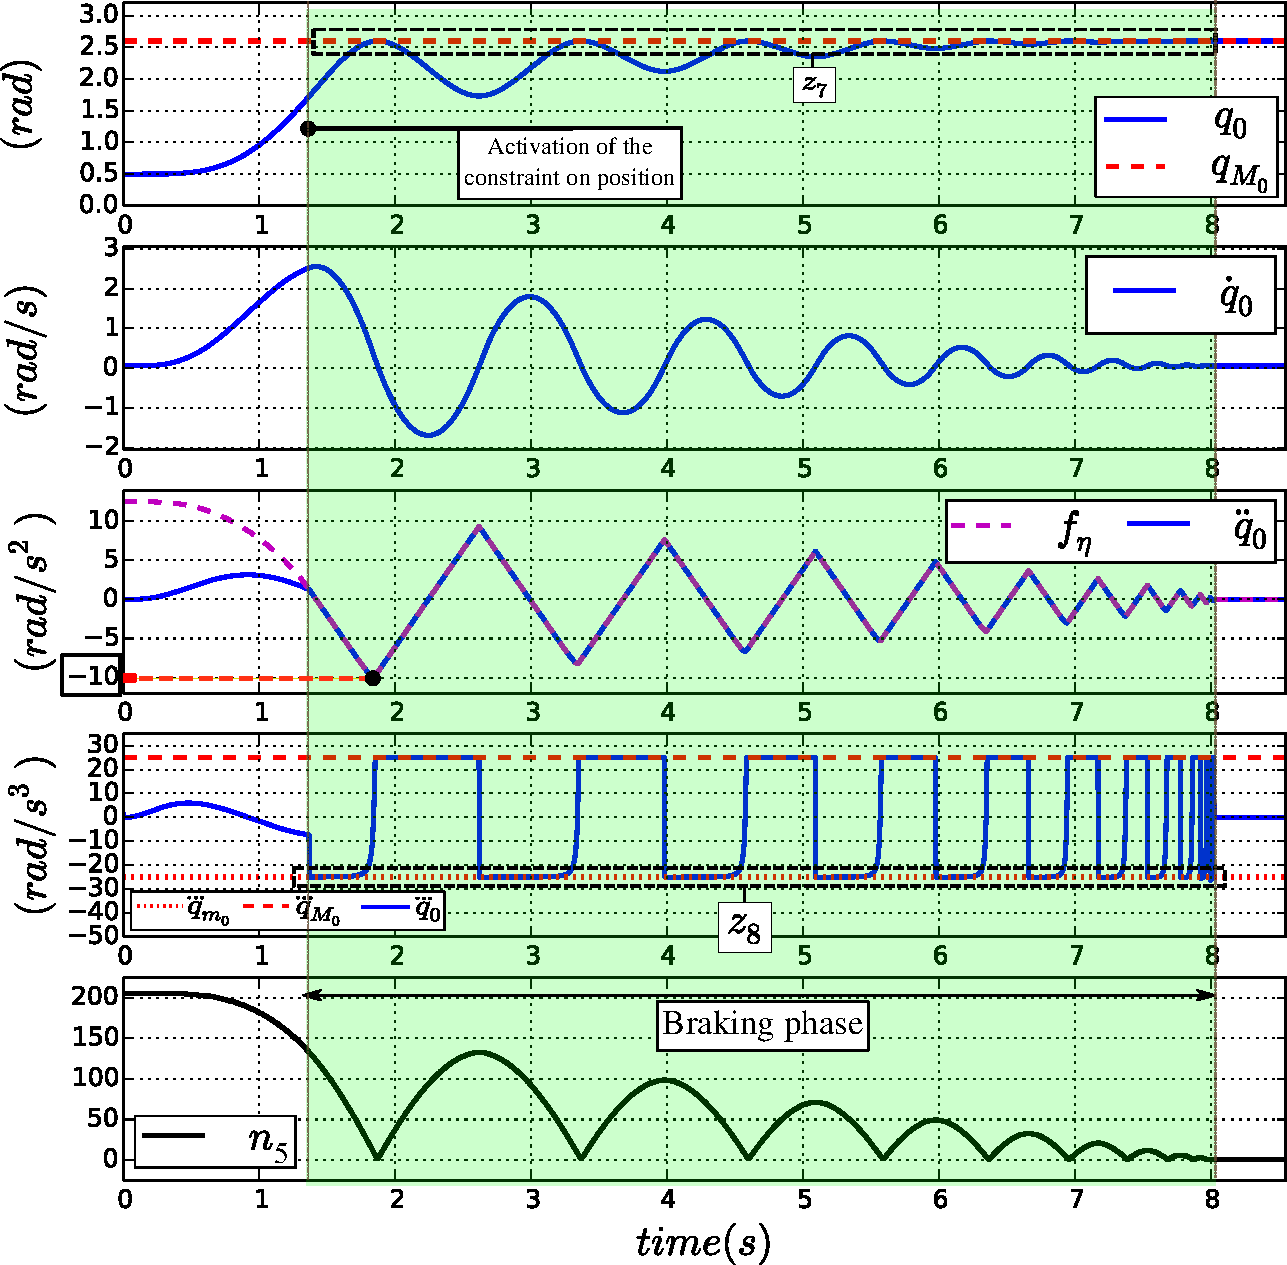
\includegraphics[width=0.8\columnwidth]{/home/anis/Desktop/THESIS_ANIS/THESIS/figures/Constrcomp/6_Posi_constr_jerk_comp_25_non_complete_formula_backklash}}
%\caption{State $S$ of joint $0$ during the braking phase to cope with a maximum position limit $q_{M_{0}}$; The new constraint formulation (\ref{eq:q_ddot_posi_jerk_comp_upp}) that takes into account the jerk capability $\dddot{q}_{m_{0}} = -25~rad.s^{-3}$ is used. Top to bottom: position, velocity, acceleration, jerk and $n_5$.} 
%\label{fig:6_Posi_constr_jerk_comp_25_non_complete_formula_backklash}
%\end{figure}
%\begin{figure}[!htbp]
%\centering
%{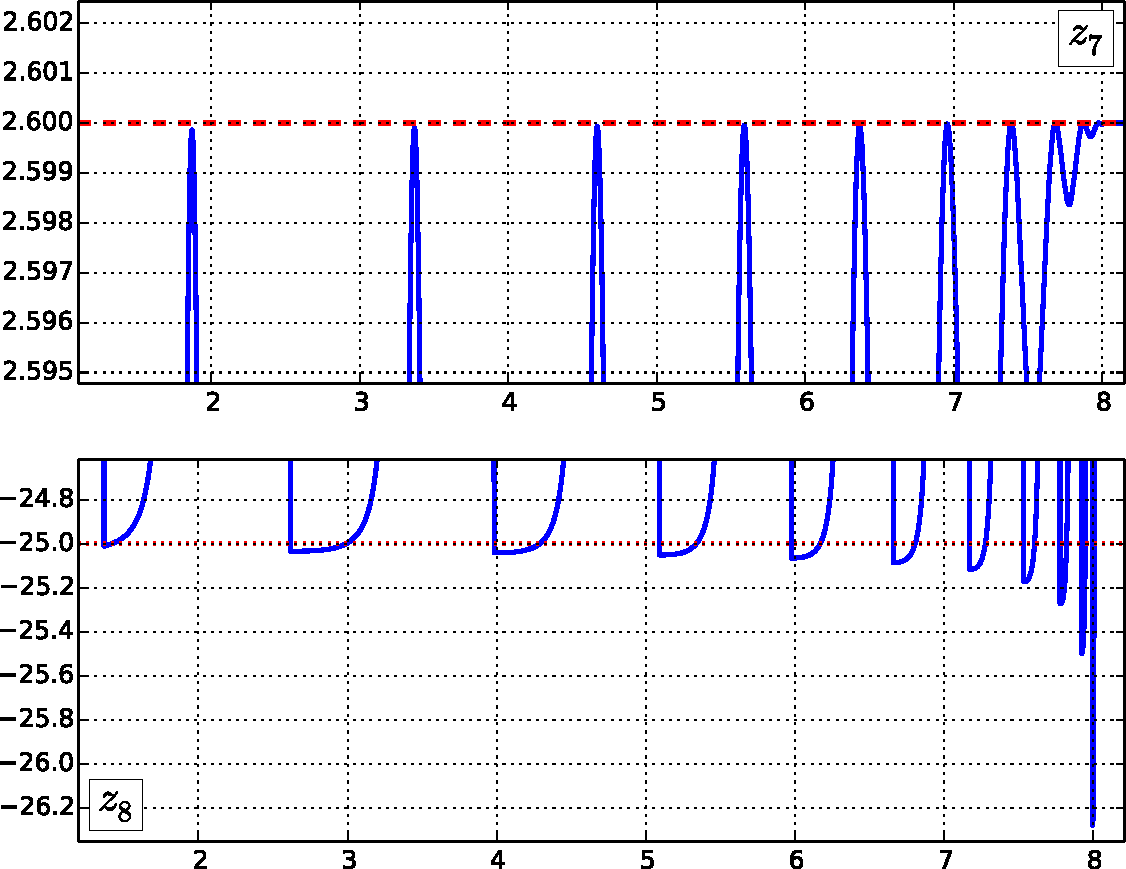
\includegraphics[width=0.8\columnwidth]{/home/anis/Desktop/THESIS_ANIS/THESIS/figures/Constrcomp/6_Posi_constr_jerk_comp_25_non_complete_formula_backklash_zoom}}
%\caption{Zooms corresponding to Fig.~\ref{fig:6_Posi_constr_jerk_comp_25_non_complete_formula_backklash}.} 
%\label{fig:6_Posi_constr_jerk_comp_25_non_complete_formula_backklash_zoom}
%\end{figure}
\begin{landscape}
\begin{figure}
\begin{minipage}[c]{0.5\linewidth}
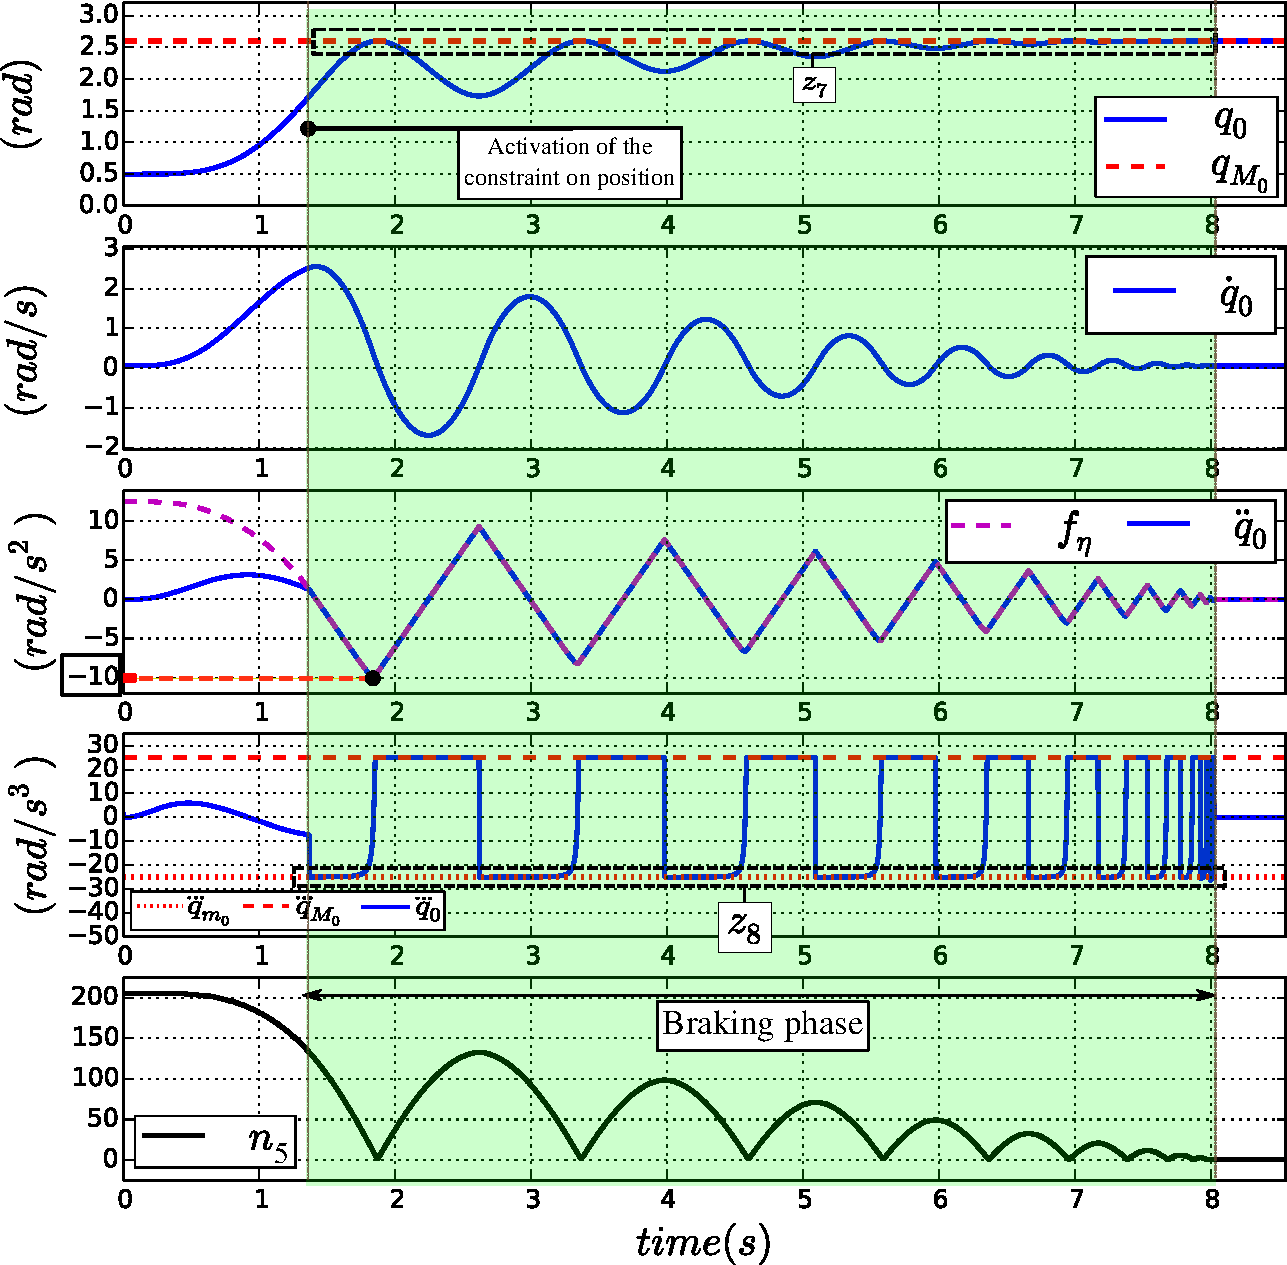
\includegraphics[width=0.99\columnwidth]{/home/anis/Desktop/THESIS_ANIS/THESIS/figures/Constrcomp/6_Posi_constr_jerk_comp_25_non_complete_formula_backklash}
\caption{Extended state $S$ of joint $0$ during the braking phase implicitly induced to cope with an upper position limit $q_{M_{0}}$. The new version of the formulation of the constraint on articular position (\ref{eq:q_ddot_posi_jerk_comp_upp}) that takes into account the jerk capability $(\dddot{q}_{m_{0}} = -25~rad.s^{-3})$ is used. Top to bottom: position, velocity, acceleration, jerk and $n_5$. See $z_7$ and $z_8$ in Fig.~\ref{fig:4_Posi_constr_acc_comp_100_zoom}.} 
\label{fig:6_Posi_constr_jerk_comp_25_non_complete_formula_backklash}
\end{minipage}
\hfill
\begin{minipage}[c]{0.5\linewidth}
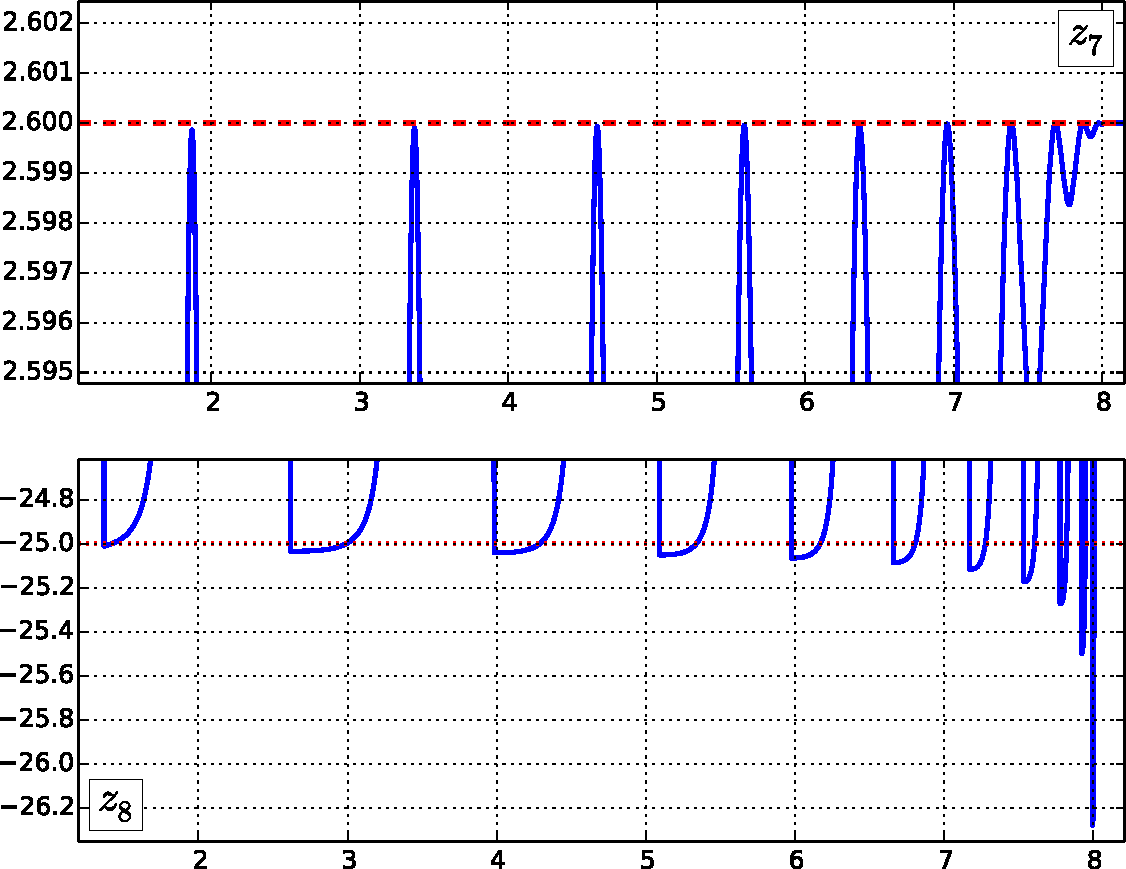
\includegraphics[width=0.90\columnwidth]{/home/anis/Desktop/THESIS_ANIS/THESIS/figures/Constrcomp/6_Posi_constr_jerk_comp_25_non_complete_formula_backklash_zoom}
\caption{Zooms corresponding to Fig.~\ref{fig:6_Posi_constr_jerk_comp_25_non_complete_formula_backklash}.} 
\label{fig:6_Posi_constr_jerk_comp_25_non_complete_formula_backklash_zoom}
\end{minipage}%
\end{figure}
\end{landscape}
%7
%\begin{figure}[!htbp]
%\centering
%{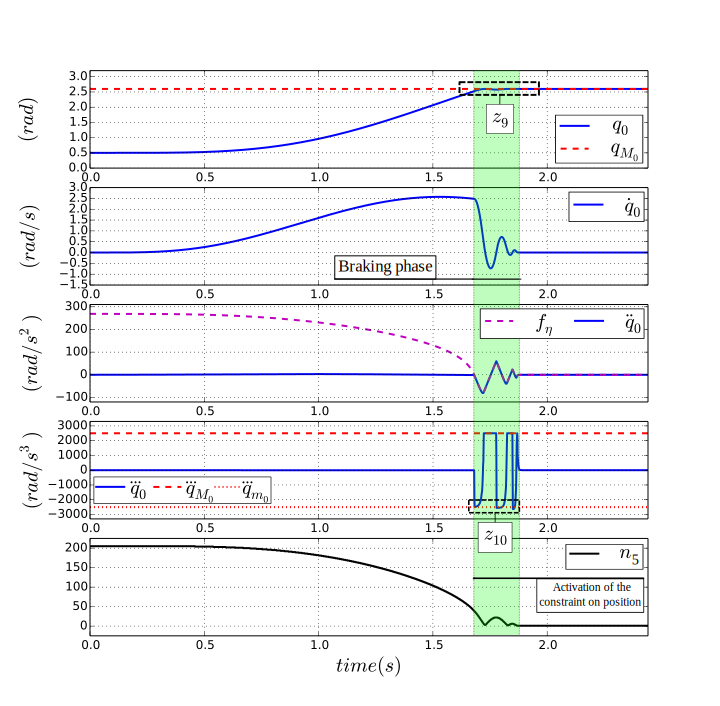
\includegraphics[width=0.8\columnwidth]{/home/anis/Desktop/THESIS_ANIS/THESIS/figures/Constrcomp/7_Posi_constr_jerk_comp_2500_non_complete_formula_backklash}}
%\caption{State $S$ of joint $0$ during the braking phase to cope with a maximum position limit; The new constraint formulation (\ref{eq:q_ddot_posi_jerk_comp_upp}) that takes into account the jerk capability $\dddot{q}_{m_{0}} = -2500~rad.s^{-3}$. Top to bottom: position, velocity, acceleration, jerk and $n_5$.} 
%\label{fig:7_Posi_constr_jerk_comp_2500_non_complete_formula_backklash}
%\end{figure}
%\begin{figure}[!htbp]
%\centering
%{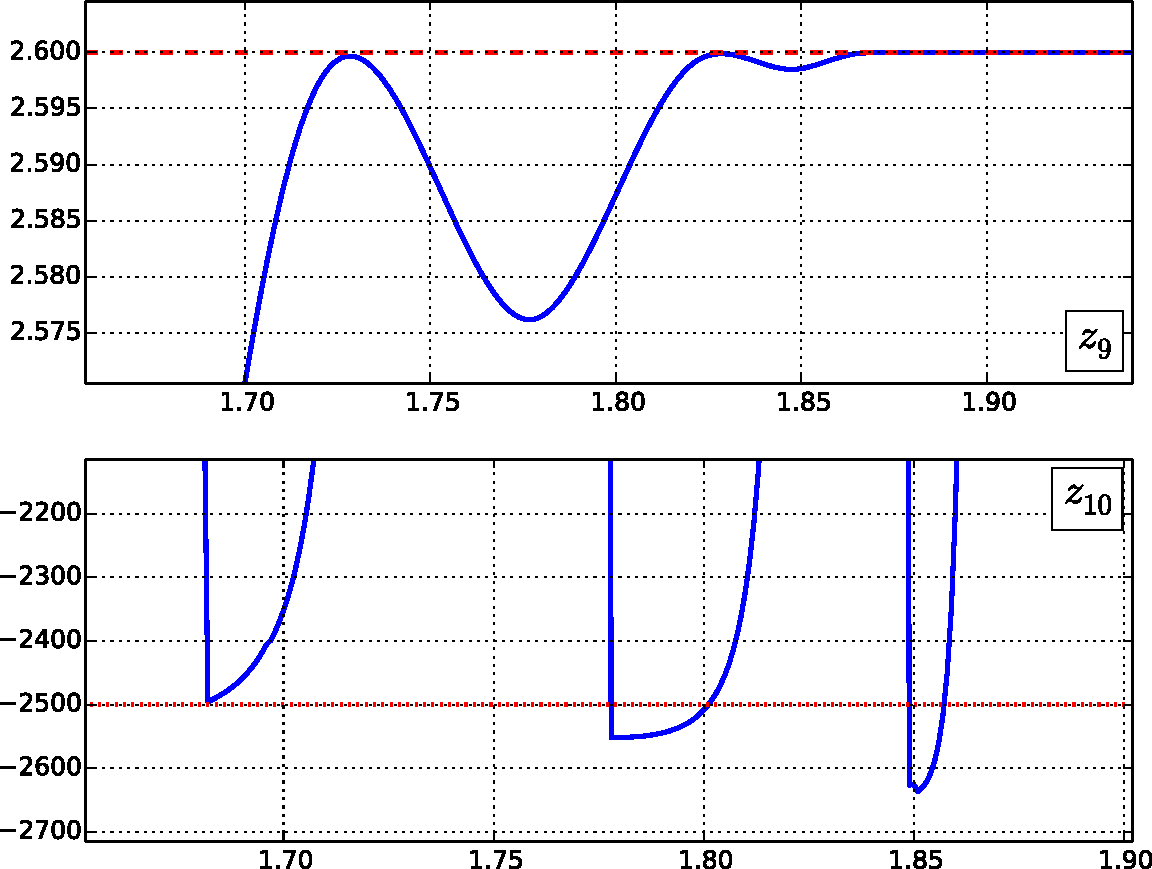
\includegraphics[width=0.7\columnwidth]{/home/anis/Desktop/THESIS_ANIS/THESIS/figures/Constrcomp/7_Posi_constr_jerk_comp_2500_non_complete_formula_backklash_zoom}}
%\caption{Zooms corresponding to Fig.~\ref{fig:7_Posi_constr_jerk_comp_2500_non_complete_formula_backklash}.} 
%\label{fig:7_Posi_constr_jerk_comp_2500_non_complete_formula_backklash_zoom}
%\end{figure}
\begin{landscape}
\begin{figure}
\begin{minipage}[c]{0.5\linewidth}
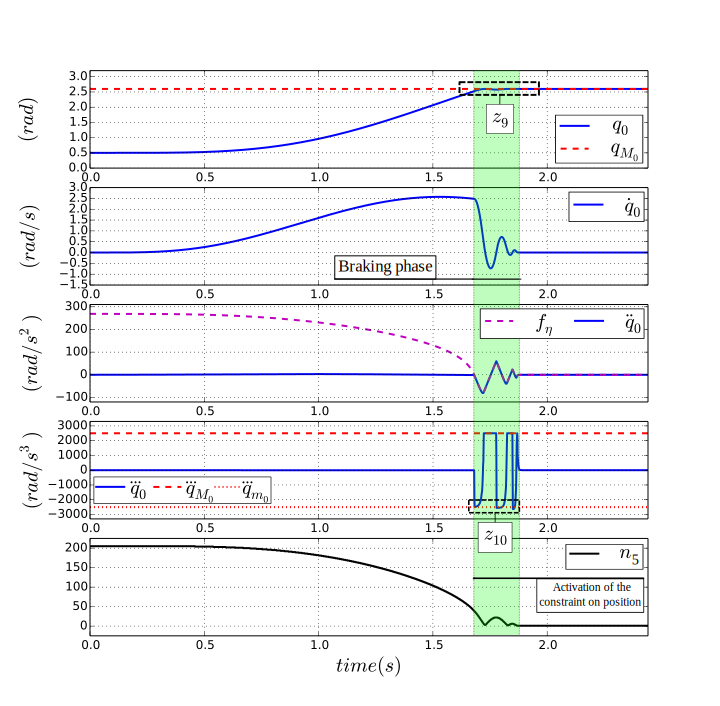
\includegraphics[width=0.99\columnwidth]{/home/anis/Desktop/THESIS_ANIS/THESIS/figures/Constrcomp/7_Posi_constr_jerk_comp_2500_non_complete_formula_backklash}
\caption{Extended state $S$ of joint $0$ during the braking phase implicitly induced to cope with an upper position limit $q_{M_{0}}$. The new version of the formulation of the constraint on articular position (\ref{eq:q_ddot_posi_jerk_comp_upp}) that takes into account the jerk capability $(\dddot{q}_{m_{0}} = -2500~rad.s^{-3})$ is used. Top to bottom: position, velocity, acceleration, jerk and $n_5$. See $z_9$ and $z_{10}$ in Fig.~\ref{fig:7_Posi_constr_jerk_comp_2500_non_complete_formula_backklash_zoom}.} 
\label{fig:7_Posi_constr_jerk_comp_2500_non_complete_formula_backklash}
\end{minipage}
\hfill
\begin{minipage}[c]{0.5\linewidth}
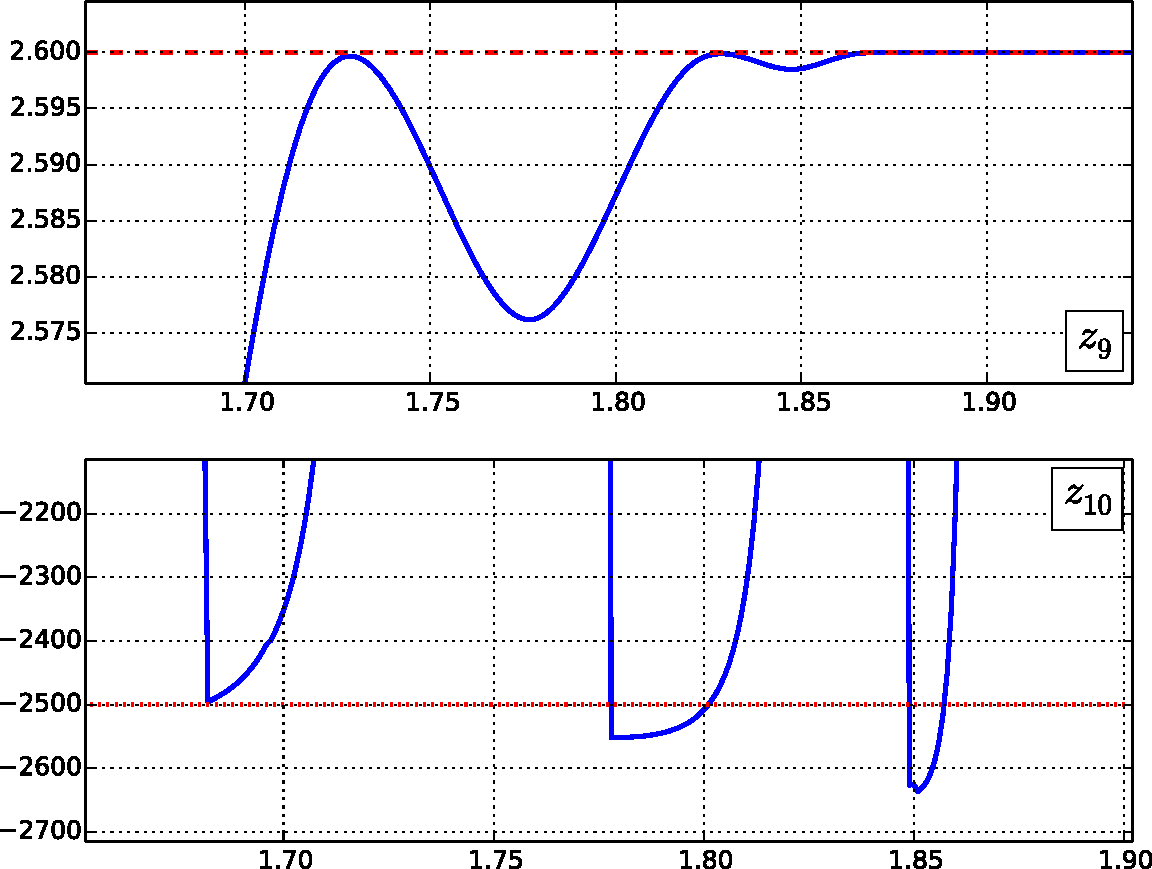
\includegraphics[width=0.90\columnwidth]{/home/anis/Desktop/THESIS_ANIS/THESIS/figures/Constrcomp/7_Posi_constr_jerk_comp_2500_non_complete_formula_backklash_zoom}
\caption{Zooms corresponding to Fig.~\ref{fig:7_Posi_constr_jerk_comp_2500_non_complete_formula_backklash}.} 
\label{fig:7_Posi_constr_jerk_comp_2500_non_complete_formula_backklash_zoom}
\end{minipage}%
\end{figure}
\end{landscape}
%%%%%%%%%%%%%%%%%%%%%%%%%%SUBSUBSECTION%%%%%%%%%%%%%%%%%%%%%%%%%%%%%
%%%%%%%%%%%%%%%%%%%%%%%%%%SUBSUBSECTION%%%%%%%%%%%%%%%%%%%%%%%%%%%%%
\subsubsection{Joint position constraint incompatibility with jerk limits 2}
\label{subsec:case3}
As previously explained, to palliate the oscillations induced on the movement of a joint when using (\ref{eq:qddot_cond_to_satisfy_Jerk_posi_compatibility}) to cope with an upper or lower position limit, a more \nameref{label:complete} description of the braking phase must be used. In this case, we consider the braking phase of a joint moving towards its upper position limit $q_{M}$, the new formulation of the constraint on its position includes both the lower $\dddot{q}_{m}$ and upper $\dddot{q}_{M}$ jerk limits. The implicitly induced braking phase that makes the joint stop at $q_{M}$ is as follows: joint $0$ starts jerking negatively with maximum producible jerk $\dddot{q}_m$ during $n_{7}$ iterations to force reduce the amount of acceleration $(\ddot{q} \geq 0)$ it contains. The reached amount of deceleration $(\ddot{q} \leq 0)$ is then progressively ``\textit{released}'' and brought to $0$ by jerking positively with maximum producible jerk $\dddot{q}_M$ during $n_{9}$ control time-steps (see Fig.~\ref{fig:8_Podfgf12}). Maximum producible deceleration $\ddot{q}_{m}$ is not considered in this case. The extended state $\textit{S}$ of the system during this implicitly induced braking phase can be described as:
\begin{equation} 
\resizebox{0.63\hsize}{!}{$
\begin{split}
\left.\begin{aligned}
\textit{S}_{|k+1}&\left\{\begin{array}{lcl}
q_{|k+1} \hspace{5mm}= q_{|k} + \dot{q}_{|k} \delta t, \\
\dot{q}_{|k+1} \hspace{5mm}= \dot{q}_{|k} + \ddot{q} \delta t, \\
\ddot{q}_{|k+1} \hspace{5mm}= \ddot{q}_{|k} + \dddot{q}_{m} \delta t;
\end{array}\right. \\
& \hspace{7mm}\vdots\ \hspace{16mm}\vdots\ \\
\textit{S}_{|k+n_{7}}&\left\{\begin{array}{lcl}
q_{|k+n_{7}} \hspace{5mm}= q_{|k+n_{7}-1} + \dot{q}_{|k+n_{7}-1} \delta t, \\
\dot{q}_{|k+n_{7}} \hspace{5mm}= \dot{q}_{|k+n_{7}-1} + \ddot{q}_{|k+n_{7}-1} \delta t, \\
\ddot{q}_{|k+n_{7}} \hspace{5mm}= \ddot{q}_{|k+n_{7}-1} + \dddot{q}_{m} \delta t;
\end{array}\right. 
\end{aligned}  \hspace{12mm}\right\}\textnormal{Equivalent to (\ref{eq:discretized_dynamics_posi_jerk_braking})}  \\[0.5cm]
\left.\begin{aligned}
\textit{S}_{|k+n_{7}+1}&\left\{\begin{array}{lcl}
q_{|k+n_{7}+1} \hspace{1mm}= q_{|k+n_{7}} + \dot{q}_{|k+n_{7}} \delta t, \\
\dot{q}_{|k+n_{7}+1} \hspace{1mm}= \dot{q}_{|k+n_{7}} + \ddot{q} \delta t, \\
\ddot{q}_{|k+n_{7}+1} \hspace{1mm}= \ddot{q}_{|k+n_{7}} + \dddot{q}_{M} \delta t;
\end{array}\right.\\
& \hspace{7mm}\vdots\ \hspace{17mm}\vdots\ \\
\textit{S}_{|k+n_{7}+n_{9}}&\left\{\begin{array}{lcl}
q_{|k+n_{7}+n_{9}} = q_{|k+n_{7}+n_{9}-1} + \dot{q}_{|k+n_{7}+n_{9}-1} \delta t, \\
\dot{q}_{|k+n_{7}+n_{9}} = \dot{q}_{|k+n_{7}+n_{9}-1} + \ddot{q}_{|k+n_{7}+n_{9}-1} \delta t, \\
\ddot{q}_{|k+n_{7}+n_{9}} = \ddot{q}_{|k+n_{7}+n_{9}-1} + \dddot{q}_{M} \delta t.
\end{array}\right.
\end{aligned} \right\}\textnormal{Equivalent to (\ref{eq:discretized_dynamics_posi_jerk_braking})}  \\[0.5cm]
\end{split}$}
\label{eq:discretized_dynamics_posi_jerk_braking_complete_formula}
\end{equation}
With: $q_{|k} \geq 0$, $\dot{q}_{|k} \geq 0$, $\dddot{q}_{m} \leq 0$ and $\dddot{q}_{M} \geq 0$. The joint position evolution in $(n_7+n_9)$ iterations is equal to the general form\footnote{Computed using Maple \cite{maple}.} of the numerical sequence (\ref{eq:discretized_dynamics_posi_jerk_braking_complete_formula}):
\begin{equation}
q_{|k+n_7+n_9} = q_{|k+n_7} + n_9 \dot{q}_{|k+n_7} \delta t +  \frac{\left(n_9^2-n_9\right)}{2} \ddot{q}_{|k+n_7} \delta t^2 + \left(\frac{n_9^3}{6}-\frac{n_9^2}{2}+\frac{n_9}{3}\right) \dddot{q}_M \delta t^3.
\label{eq:q_evolution_with_const_qdddot_m_const_qdddot_M}
\end{equation}
With $q_{|k+n_{7}}$ and $\dot{q}_{|k+n_{7}}$, respectively equivalent to (\ref{eq:q_evolution_with_const_qdddot_m}) and (\ref{eq:q_dot_evolution_with_const_qdddot_m}). And: 
\begin{equation}
\ddot{q}_{|k+n_7} = \ddot{q}_{|k} + n_{7} \dddot{q}_m \delta t.
\label{eq:q_ddot_evo_in_n_7_iteration_q_dddot_m}
\end{equation}
When developed, (\ref{eq:q_evolution_with_const_qdddot_m_const_qdddot_M}) is written:
\begin{equation}
\begin{split}
q_{|k+n_7+n_9} = q_{|k} & + \left(n_7+n_9\right) \dot{q}_{|k} \delta t + \left[\left(n_7 n_9\right)+\frac{\left(n_{7}^{2}-n_7\right)+\left(n_{9}^{2}-n_9\right)}{2}\right] \ddot{q}_{|k} \delta t^2 \\
& + \left[\frac{n_{7}\left(n_{9}^{2}-n_9\right)+n_{9}\left(n_{7}^{2}-n_7\right)}{2}+\left(\frac{n_{7}^{3}}{6}-\frac{n_{7}^{2}}{2}+\frac{n_{7}}{3}\right)\right] \dddot{q}_m \delta t^3 \\
& + \left(\frac{n_{9}^{3}}{6}-\frac{n_{9}^{2}}{2}+\frac{n_{9}}{3}\right) \dddot{q}_M \delta t^3.
\end{split}
\label{eq:q_evolution_with_const_qdddot_m_const_qdddot_M_dev}
\end{equation}
Finally, the condition $q_{|k+n_7+n_9} \leq q_{M}$ for all integers $(n_7, n_9)$ leads to:
\begin{equation}
\begin{split}
\ddot{q}_{|k}^{c} \leq & \frac{\left(q_M-q_{|k}\right)}{\left[\left(n_7 n_9\right)+\frac{\left(n_{7}^{2}-n_7\right)+\left(n_{9}^{2}-n_9\right)}{2}\right] \delta t^2} + \frac{\left(n_7+n_9\right) \dot{q}_{|k}}{\left[\left(n_7 n_9\right)+\frac{\left(n_{7}^{2}-n_7\right)+\left(n_{9}^{2}-n_9\right)}{2}\right] \delta t} \\
& + \frac{\left[\frac{n_{7}\left(n_{9}^{2}-n_9\right)+n_{9}\left(n_{7}^{2}-n_7\right)}{2}+\left(\frac{n_{7}^{3}}{6}-\frac{n_{7}^{2}}{2}+\frac{n_{7}}{3}\right)\right] \dddot{q}_m \delta t}{\left[\left(n_7 n_9\right)+\frac{\left(n_{7}^{2}-n_7\right)+\left(n_{9}^{2}-n_9\right)}{2}\right]} \\
& + \frac{\left(\frac{n_{9}^{3}}{6}-\frac{n_{9}^{2}}{2}+\frac{n_{9}}{3}\right) \dddot{q}_M \delta t}{\left[\left(n_7 n_9\right)+\frac{\left(n_{7}^{2}-n_7\right)+\left(n_{9}^{2}-n_9\right)}{2}\right]}.
\end{split}
\label{eq:q_constr_on_q_ddot_with_const_qdddot_m_const_qdddot_M_1}
\end{equation}
$(n_7, n_9)$ are the two integers minimizing the right-hand side of (\ref{eq:q_constr_on_q_ddot_with_const_qdddot_m_const_qdddot_M_1}).
Following the same reasoning for the lower position limit, the condition $q_{|k+n_8+n_{10}} \geq q_{m}$ can be reflected on the acceleration control variable as:
\begin{equation}
\begin{split}
\ddot{q}_{|k}^{c} \geq & \frac{\left(q_m-q_{|k}\right)}{\left[\left(n_8 n_{10}\right)+\frac{\left(n_{8}^{2}-n_8\right)+\left(n_{10}^{2}-n_{10}\right)}{2}\right] \delta t^2} + \frac{\left(n_8+n_{10}\right) \dot{q}_{|k}}{\left[\left(n_8 n_{10}\right)+\frac{\left(n_{8}^{2}-n_8\right)+\left(n_{10}^{2}-n_{10}\right)}{2}\right] \delta t} \\
& + \frac{\left[\frac{n_{8}\left(n_{10}^{2}-n_{10}\right)+n_{10}\left(n_{8}^{2}-n_8\right)}{2}+\left(\frac{n_{8}^{3}}{6}-\frac{n_{8}^{2}}{2}+\frac{n_{8}}{3}\right)\right] \dddot{q}_M \delta t}{\left[\left(n_8 n_{10}\right)+\frac{\left(n_{8}^{2}-n_8\right)+\left(n_{10}^{2}-n_{10}\right)}{2}\right]} \\
& + \frac{\left(\frac{n_{10}^{3}}{6}-\frac{n_{10}^{2}}{2}+\frac{n_{10}}{3}\right) \dddot{q}_m \delta t}{\left[\left(n_8 n_{10}\right)+\frac{\left(n_{8}^{2}-n_8\right)+\left(n_{10}^{2}-n_{10}\right)}{2}\right]}, 
\end{split}
\label{eq:q_constr_on_q_ddot_with_const_qdddot_M_const_qdddot_m_2}
\end{equation}
with $(n_8, n_{10})$: the two integers maximizing the right-hand side of (\ref{eq:q_constr_on_q_ddot_with_const_qdddot_m_const_qdddot_M_1}). \\ $\textit{f}_{\mu}$ and $\textit{f}_{\lambda}$ are respectively equivalent to the right-hand sides of (\ref{eq:q_constr_on_q_ddot_with_const_qdddot_M_const_qdddot_m_2}) and (\ref{eq:q_constr_on_q_ddot_with_const_qdddot_m_const_qdddot_M_1}). \\ 
\noindent\begin{minipage}{\textwidth}
\renewcommand\footnoterule{}                  %% This line should come here.
\begin{algorithm}[H]
\caption{Compute $n_{7}, n_{8}, n_{9}, n_{10}, f_{\mu}$ and $f_{\lambda}$}
\label{alg:compute_f_mu_f_lambda_n_7_n_8_n_9_n_10}
\begin{algorithmic}[1]
%f_{\mu}(n_{8},  n_{10})     f_{\lambda}(n_{7},  n_{9})
%    n1_pos  n2_pos          n1_neg  n2_neg
\Require $q_M, q_m, q_{|k}, \dot{q}_{|k},\dddot{q}_{M},\dddot{q}_{m}, \delta t$
\myState{$f_{{\mu}_{max}} \gets \ddot{q}_{m}$} \Comment{temporary lower bound of $\ddot{q}_{|k}^{c}$}
\myState{$f_{{\lambda}_{min}} \gets \ddot{q}_{M}$} \Comment{temporary upper bound of $\ddot{q}_{|k}^{c}$}
\For{($i = 1 \rightarrow N$)}
        \myState{$n_{8}^{*} \gets i \qquad n_{7}^{*} \gets i$}
%        \If{($\ddot{q}_{|k} \geq 0$)} 
%             \State{$n_{9}^{*} \gets n_{7}^{*}-\abs[\Big]{\myfrac[5pt]{\ddot{q}_{|k}}{\dddot{q}_m \delta t}} \qquad n_{10}^{*} \gets n_{8}^{*}+\abs[\Big]{\myfrac[5pt]{\ddot{q}_{|k}}{\dddot{q}_M \delta t}}$}
%        \EndIf 
\IfThenElse{($\ddot{q}_{|k} \geq 0$)}% If ...
            {$n_{9}^{*} \gets n_{7}^{*}-\abs[\Big]{\myfrac[5pt]{\ddot{q}_{|k}}{\dddot{q}_m \delta t}} \qquad n_{10}^{*} \gets n_{8}^{*}+\abs[\Big]{\myfrac[5pt]{\ddot{q}_{|k}}{\dddot{q}_M \delta t}}$}% ...then...        
        \If{($\ddot{q}_{|k} < 0$)} 
           \State{$n_{9}^{*} \gets n_{7}^{*}+\abs[\Big]{\myfrac[5pt]{\ddot{q}_{|k}}{\dddot{q}_M \delta t}} \qquad n_{10}^{*} \gets n_{8}^{*}-\abs[\Big]{\myfrac[5pt]{\ddot{q}_{|k}}{\dddot{q}_m \delta t}}$}
%            \If{($n_{7}^{*} \leq 1$)}
%                \myState{$n_{9}^{*} \gets \abs[\Big]{\myfrac[5pt]{\ddot{q}_{|k}}{\dddot{q}_M \delta t}}$}           
%            \EndIf
            \IfThenElse{($n_{7}^{*} \leq 1$)}% If ...
            {$n_{9}^{*} \hspace{1.5mm}\gets \abs[\Big]{\myfrac[5pt]{\ddot{q}_{|k}}{\dddot{q}_M \delta t}}$}% ...then...    
%            \If{($n_{8}^{*} \leq 1$)}     
%                \myState{$n_{10}^{*} \gets \abs[\Big]{\myfrac[5pt]{\ddot{q}_{|k}}{\dddot{q}_m \delta t}}$}            
%            \EndIf                
\vspace{2mm}
            \IfThenElse{($n_{8}^{*} \leq 1$)}% If ...
            {$n_{10}^{*} \gets \abs[\Big]{\myfrac[5pt]{\ddot{q}_{|k}}{\dddot{q}_m \delta t}}$}% ...then...     
        \EndIf
\IfThenElse{($n_{7}^{*} \hspace{1mm}\leq 1$)}% If ...
            {$n_{7}^{*} \hspace{1.5mm}\gets 1$}% ...then...
\IfThenElse{($n_{8}^{*} \hspace{1mm}\leq 1$)}% If ...
            {$n_{8}^{*} \hspace{1.5mm}\gets 1$}% ...then...            
\IfThenElse{($n_{9}^{*} \hspace{1mm}\leq 2$)}% If ...
            {$n_{9}^{*} \hspace{1.5mm}\gets 2$}% ...then...
\IfThenElse{($n_{10}^{*} \leq 2$)}% If ...
            {$n_{10}^{*} \gets 2$}% ...then...            
        \myState{$f_{\mu}^{*} \gets f_{\mu}(q_m, \dddot{q}_M, q_{|k}, \dot{q}_{|k}, \dddot{q}_m, n_{8}^{*}, n_{10}^{*})$} 
        \myState{$f_{\lambda}^{*} \gets f_{\lambda}(q_M, \dddot{q}_m, q_{|k}, \dot{q}_{|k}, \dddot{q}_M, n_{7}^{*}, n_{9}^{*})$}
        \If{($f_{\mu}^{*} \geq f_{{\mu}_{max}}$)}
            \State{$f_{{\mu}_{max}} \gets f_{\mu}^{*} \qquad n_{8} \gets n_{8}^{*} \qquad n_{10}$\footnote{\label{note1} For stability in the computation of $f_{\mu}$ and $f_{\lambda}$, ($n_{9}^{*}, n_{10}^{*}$) are used as real numbers (even if previously defined as numbers of iterations). The same for $n_{9}$ and $n_{10}$.} $\gets n_{10}^{*}$}
        \EndIf   
        \If{($f_{\lambda}^{*} \leq f_{{\lambda}_{min}}$)}
            \State{$f_{{\lambda}_{min}} \gets f_{\lambda}^{*} \qquad n_{7} \gets n_{7}^{*} \qquad n_{9}\footnoteref{note1} \gets n_{9}^{*}$}
        \EndIf            
\EndFor
\State{$f_{\mu} \gets f_{{\mu}_{max}} \qquad f_{\lambda} \gets f_{{\lambda}_{min}}$}
\myState \Return{$n_{7}, n_{9}, n_{9}, n_{10}, f_{\mu}, f_{\lambda}$}\;
\end{algorithmic}
\end{algorithm}
\end{minipage} \\
\\
$n_{7}, n_{8}, n_{9}, n_{10}, f_{\mu}$ and $f_{\lambda}$ can be computed numerically as shown by Algorithm~\ref{alg:compute_f_mu_f_lambda_n_7_n_8_n_9_n_10}. N in Algorithm~\ref{alg:compute_f_mu_f_lambda_n_7_n_8_n_9_n_10} is fixed heuristically, it must however be $\geq$ to the total number of iterations needed to perform the braking movement described in (\ref{eq:discretized_dynamics_posi_jerk_braking_complete_formula}). More details on how to compute this parameter in Section~\ref{sec:concl_comp_cnstr}.
%********************************************************************%
\paragraph{Illustration 4}
For this simulation, using the test case scenario, the controller is implemented with the new version of the formulation of the constraint on articular position (\ref{eq:q_constr_on_q_ddot_with_const_qdddot_m_const_qdddot_M_1}), that takes  into account both the positive and negative jerk capabilities $([\dddot{q}_{m_{0}}, \dddot{q}_{M_{0}}] = [-25, 25]~rad.s^{-3})$. In this case, joint $0$ is also moving towards its upper position limit $q_{M_{0}}$. 

Fig.~\ref{fig:8_Posi_constr_jerk_comp_25_complete_formula_no_backklash} depicts how joint $0$ starts braking with maximum producible negative (sub-phase \circled{1}) then positive (sub-phase \circled{2}) jerk until reaching its upper position limit. The amount of ``\textit{charged}'' deceleration is then released and brought to $0$ as the joint stops its motion at $q_{M_{0}}$. We also highlight that in this case, no oscillations are induced when using this \textit{more complete} description of the braking phase for the formulation of the constraint on articular position. \\ 
On the other hand, we underline an exceeding of $0.013~rad.s^{-3}$ over the lower jerk limit $(\dddot{q}_{m_{0}} = -25~rad.s^{-3})$ (see Fig.~\ref{fig:8_Posi_constr_jerk_comp_25_complete_formula_no_backklash_zoom}). Also, as it appears in the articular jerk profile, the positive jerk capability is not used to its full potential for the ``\textit{de-charging}'' of the accumulated deceleration sub-phase. Which is mainly caused by the \textit{discrete} description of the state of joint $0$ during its braking phase (\ref{eq:discretized_dynamics_posi_jerk_braking_complete_formula}) and consequently the discrete new formulation of the articular position constraint.
%8
%\begin{figure}[!htbp]
%\centering
%{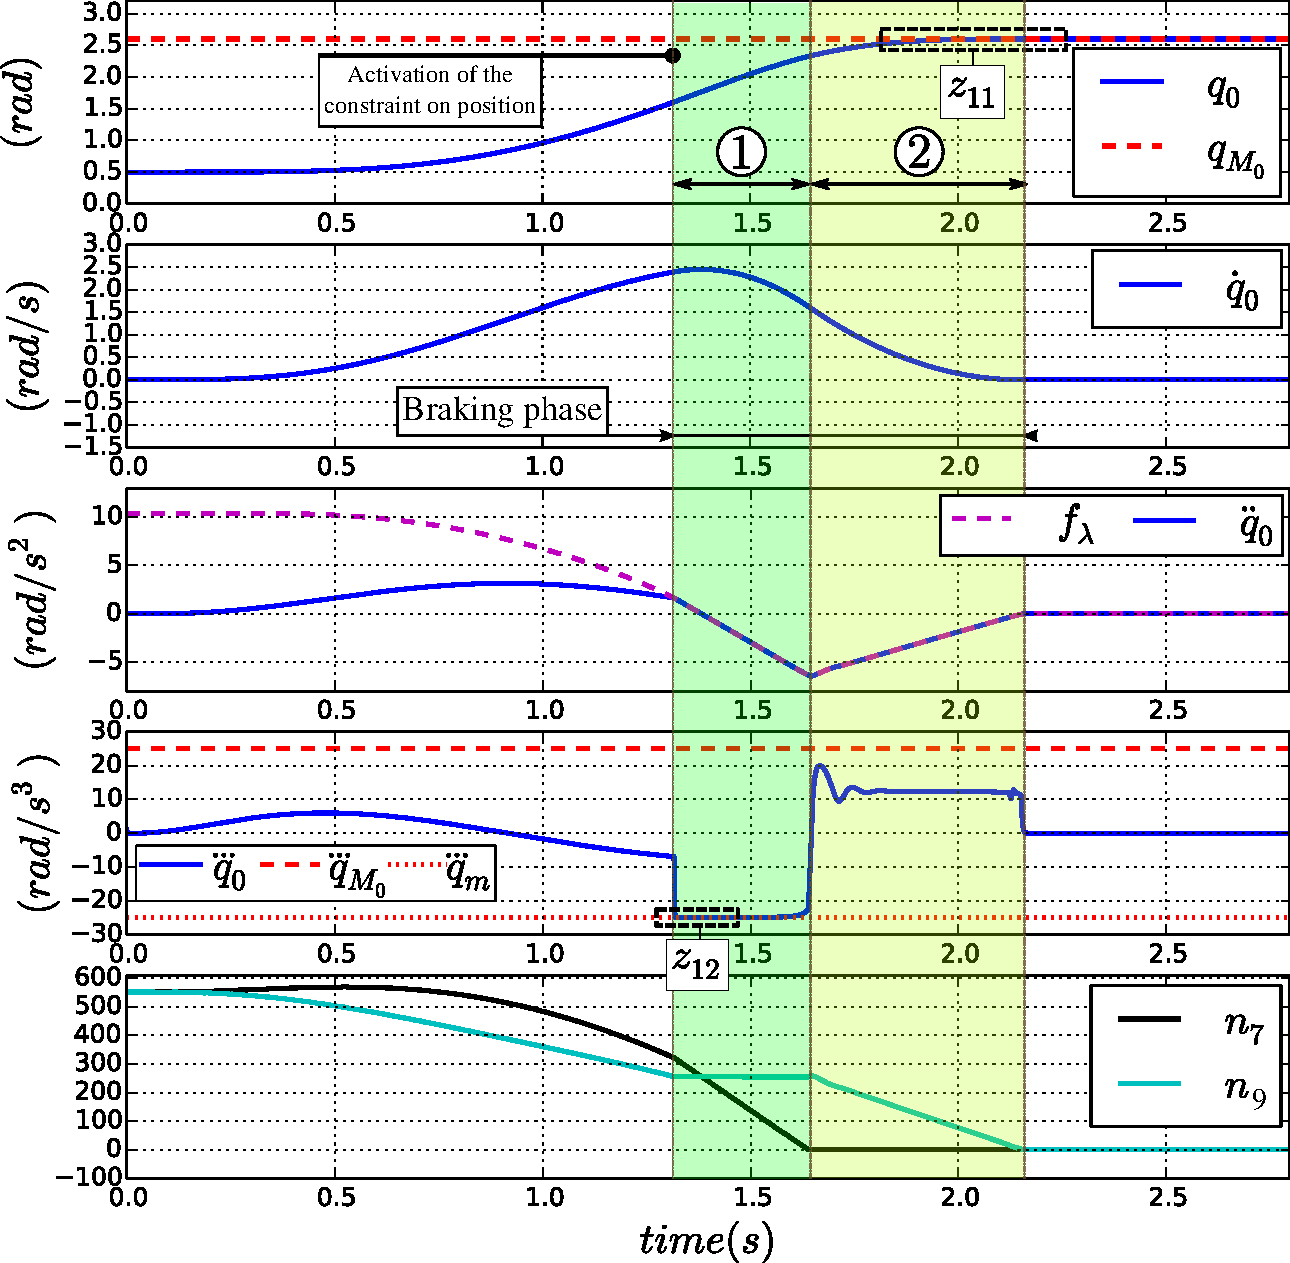
\includegraphics[width=0.8\columnwidth]{/home/anis/Desktop/THESIS_ANIS/THESIS/figures/Constrcomp/8_Posi_constr_jerk_comp_25_complete_formula_no_backklash}}
%\caption{State $S$ of joint $0$ during the braking phase to cope with a maximum position limit $q_{M_{0}}$; The new constraint formulation (\ref{eq:q_constr_on_q_ddot_with_const_qdddot_m_const_qdddot_M_1}) that takes into account both positive and negative jerk capabilities $[\dddot{q}_{m_{0}}, \dddot{q}_{M_{0}}] = [-25, 25]~rad.s^{-3}$ is used. Top to bottom: position, velocity, acceleration, jerk and ($n_7$, $n_9$).} 
%\label{fig:8_Posi_constr_jerk_comp_25_complete_formula_no_backklash}
%\end{figure}
%\begin{figure}[!htbp]
%\centering
%{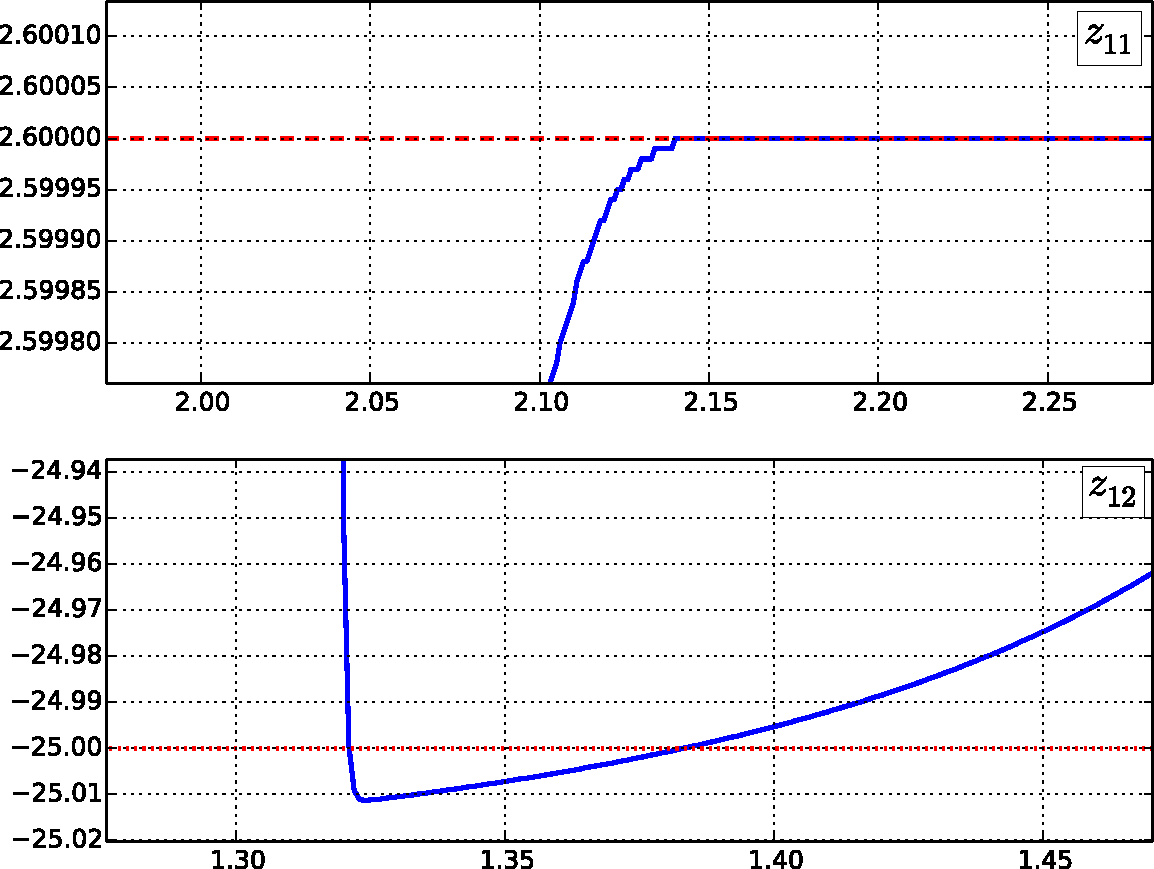
\includegraphics[width=0.8\columnwidth]{/home/anis/Desktop/THESIS_ANIS/THESIS/figures/Constrcomp/8_Posi_constr_jerk_comp_25_complete_formula_no_backklash_zoom}}
%\caption{Zooms corresponding to Fig.~\ref{fig:8_Posi_constr_jerk_comp_25_complete_formula_no_backklash}.} 
%\label{fig:8_Posi_constr_jerk_comp_25_complete_formula_no_backklash_zoom}
%\end{figure}
%
\begin{figure}[!htbp]
\centering
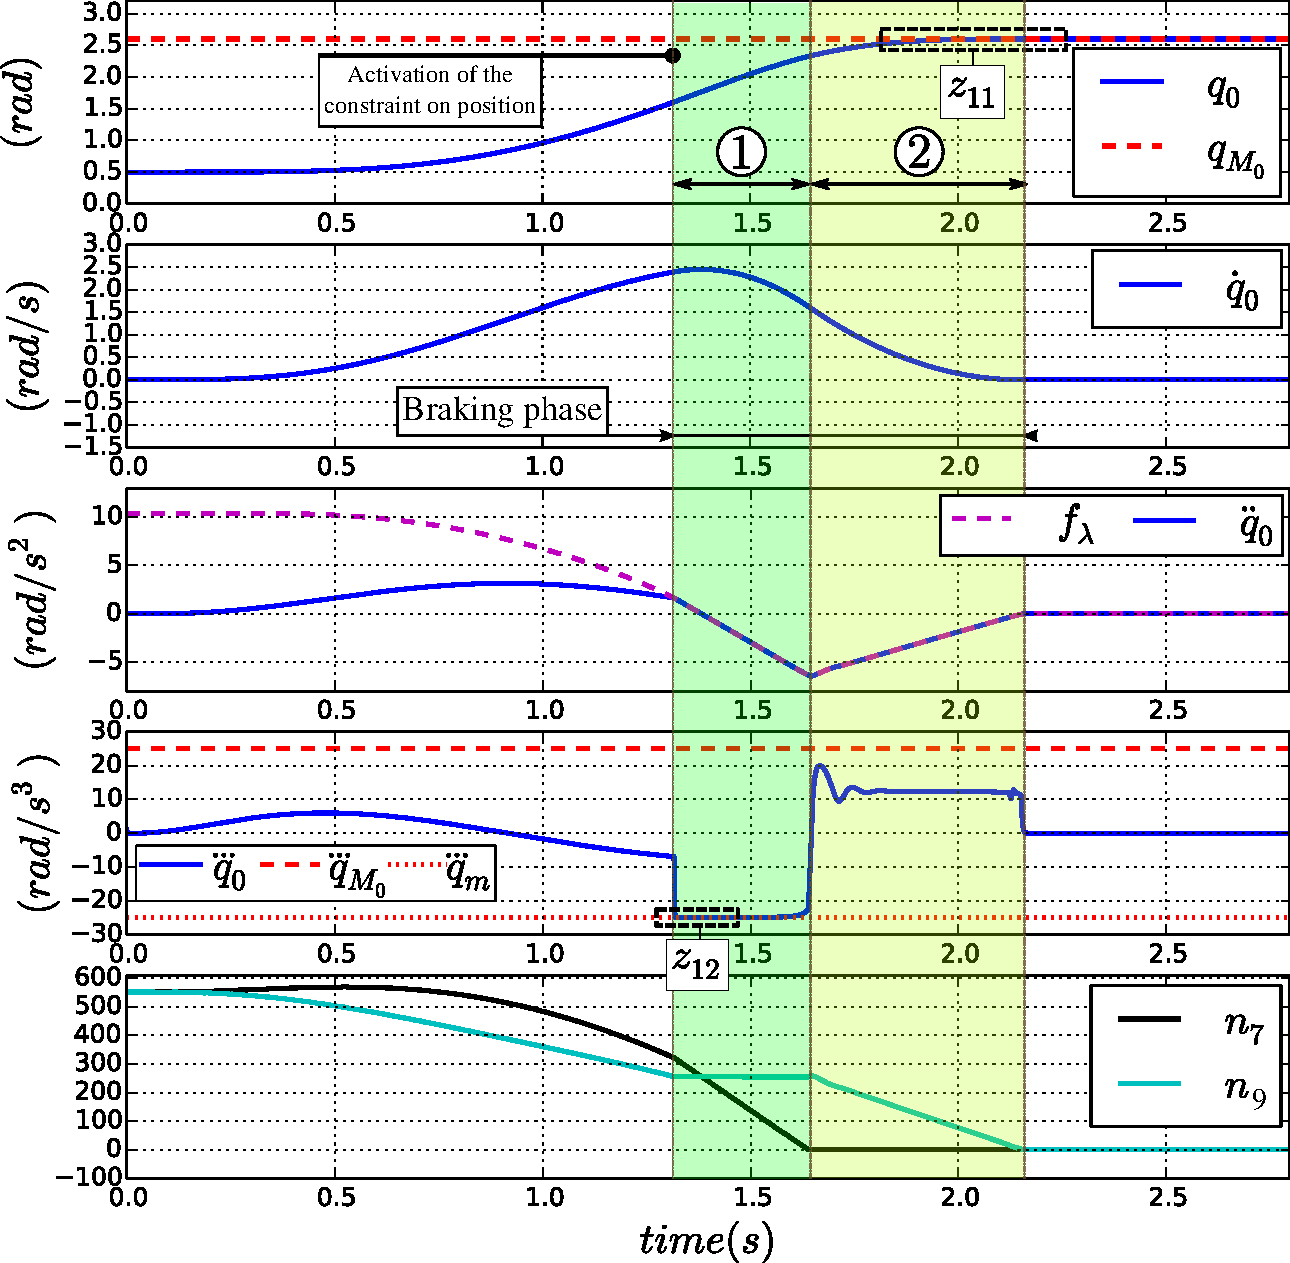
\includegraphics[width=0.99\columnwidth]{/home/anis/Desktop/THESIS_ANIS/THESIS/figures/Constrcomp/8_Posi_constr_jerk_comp_25_complete_formula_no_backklash}
\caption{Extended state $S$ of joint $0$ during the braking phase implicitly induced to cope with an upper position limit $q_{M_{0}}$. The new formulation of the constraint on articular position (\ref{eq:q_constr_on_q_ddot_with_const_qdddot_m_const_qdddot_M_1}) that takes into account both the positive and negative jerk capabilities $[\dddot{q}_{m_{0}}, \dddot{q}_{M_{0}}] = [-25, 25]~rad.s^{-3}$ is used. Top to bottom: position, velocity, acceleration, jerk and ($n_7$, $n_9$). See $z_{10}$ and $z_{11}$ in Fig.~\ref{fig:8_Posi_constr_jerk_comp_25_complete_formula_no_backklash_zoom}.} 
\label{fig:8_Posi_constr_jerk_comp_25_complete_formula_no_backklash}
\end{figure}
\begin{figure}[!htbp]
\centering
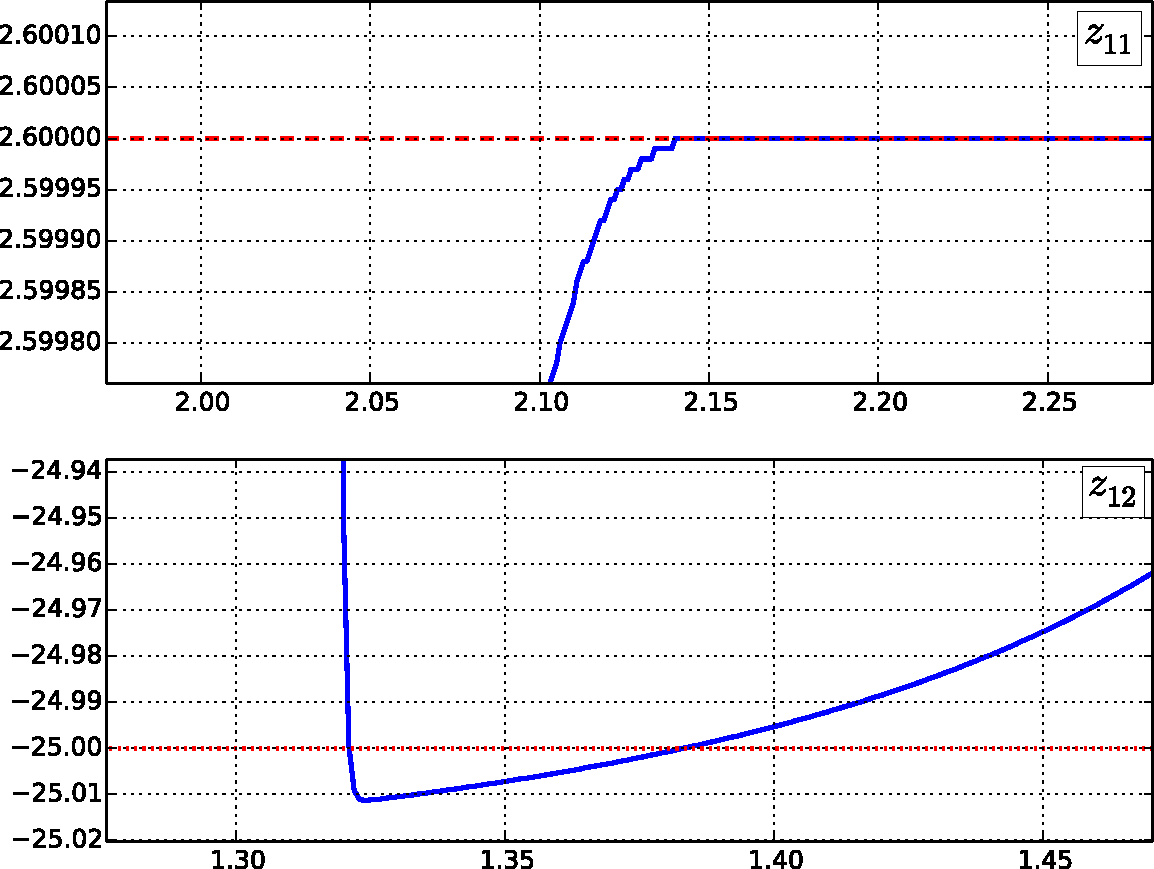
\includegraphics[width=0.90\columnwidth]{/home/anis/Desktop/THESIS_ANIS/THESIS/figures/Constrcomp/8_Posi_constr_jerk_comp_25_complete_formula_no_backklash_zoom}
\caption{Zooms corresponding to Fig.~\ref{fig:8_Posi_constr_jerk_comp_25_complete_formula_no_backklash}.} 
\label{fig:8_Posi_constr_jerk_comp_25_complete_formula_no_backklash_zoom}
\end{figure}
%
%\begin{landscape}
%\begin{figure}
%\begin{minipage}[c]{0.5\linewidth}
%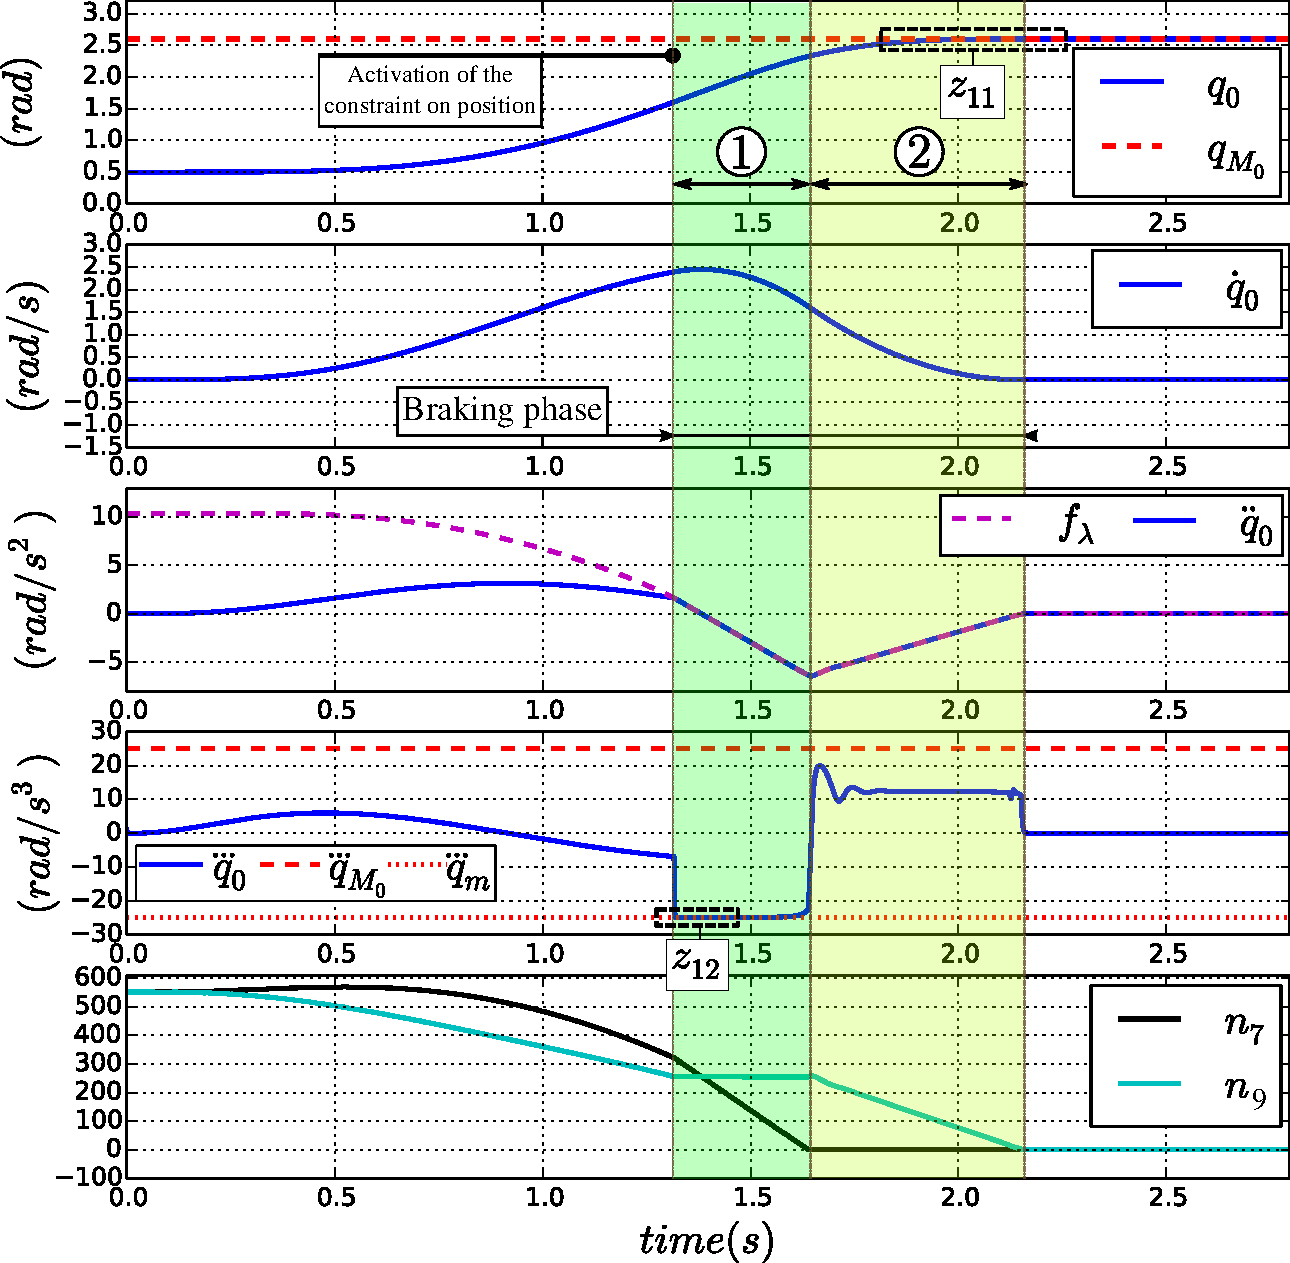
\includegraphics[width=0.99\columnwidth]{/home/anis/Desktop/THESIS_ANIS/THESIS/figures/Constrcomp/8_Posi_constr_jerk_comp_25_complete_formula_no_backklash}
%\caption{Extended state $S$ of joint $0$ during the braking phase implicitly induced to cope with an upper position limit $q_{M_{0}}$. The new formulation of the constraint on articular position (\ref{eq:q_constr_on_q_ddot_with_const_qdddot_m_const_qdddot_M_1}) that takes into account both the positive and negative jerk capabilities $[\dddot{q}_{m_{0}}, \dddot{q}_{M_{0}}] = [-25, 25]~rad.s^{-3}$ is used. Top to bottom: position, velocity, acceleration, jerk and ($n_7$, $n_9$).} 
%\label{fig:8_Posi_constr_jerk_comp_25_complete_formula_no_backklash}
%\end{minipage}
%\hfill
%\begin{minipage}[c]{0.5\linewidth}
%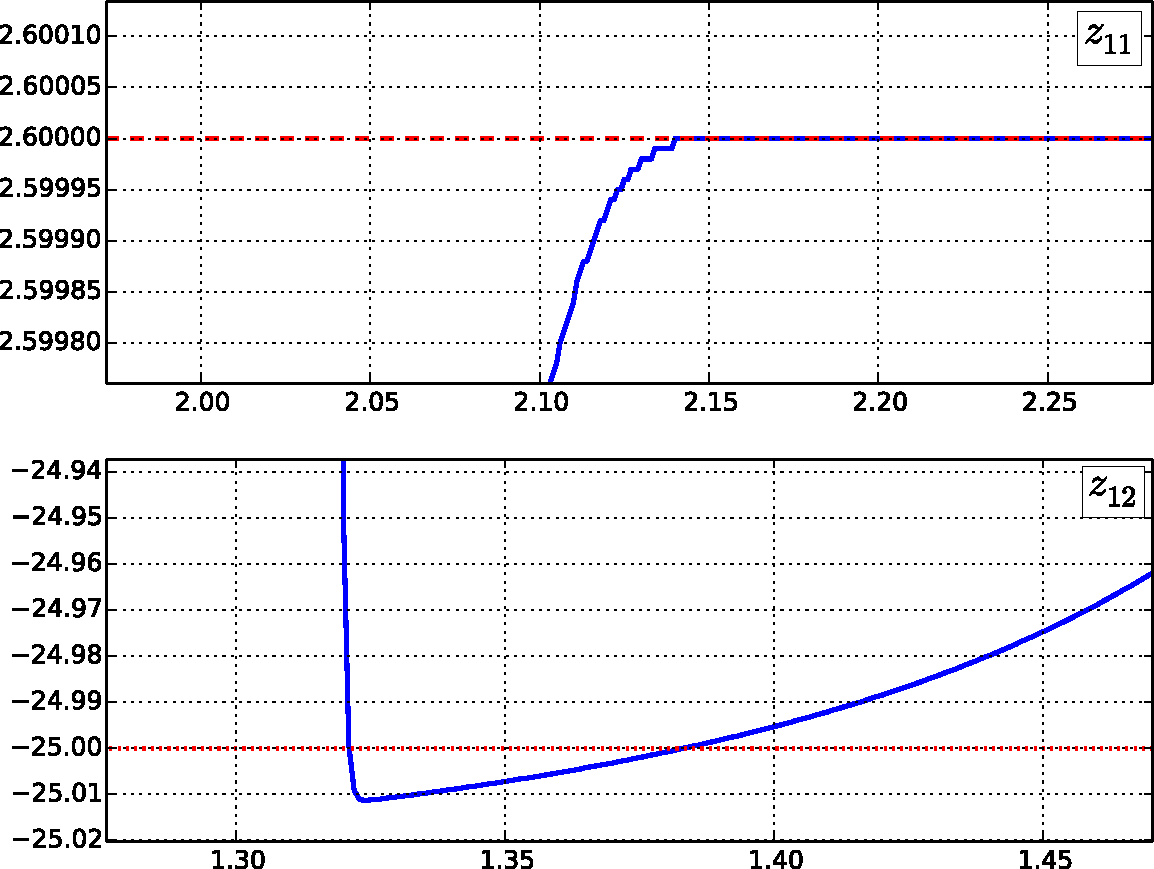
\includegraphics[width=0.90\columnwidth]{/home/anis/Desktop/THESIS_ANIS/THESIS/figures/Constrcomp/8_Posi_constr_jerk_comp_25_complete_formula_no_backklash_zoom}
%\caption{Zooms corresponding to Fig.~\ref{fig:8_Posi_constr_jerk_comp_25_complete_formula_no_backklash}.} 
%\label{fig:8_Posi_constr_jerk_comp_25_complete_formula_no_backklash_zoom}
%\end{minipage}%
%\end{figure}
%\end{landscape}
%%%%%%%%%%%%%%%%%%%%%%%%%%SUBSUBSECTION%%%%%%%%%%%%%%%%%%%%%%%%%%%%%
%%%%%%%%%%%%%%%%%%%%%%%%%%SUBSUBSECTION%%%%%%%%%%%%%%%%%%%%%%%%%%%%%
\subsubsection{Joint position constraint incompatibility with both deceleration and jerk limits 1}
\label{subsec:case4}
In all the previously introduced new formulations, the articular jerk and deceleration capabilities have been independently considered for the different mathematical expressions of the constraint on articular position. As explained in Section~\ref{subsec:complete_b_ph} regarding the description of the \nameref{label:complete} braking phase needed to \textit{\textbf{properly}} cope with an articular position limit, these capabilities $(\ddot{q}_m, \dddot{q}_m, \dddot{q}_M)$, considering an upper position limit $q_M$, should all appear together in the expression of the constraint on articular position. During the needed braking phase, the joint starts jerking negatively with maximum producible jerk $\dddot{q}_m$ during $n_{11}$ iterations. If maximum deceleration $\ddot{q}_m$ is reached, the joint brings its articular jerk to $0$ and the ``\textit{charged}'' deceleration $(\dddot{q} = \dddot{q}_m)$ is applied for $n_{13}$ iterations. Finally, the amount of deceleration in the joint is ``\textit{de-charged}'' and released during several time-steps by jerking positively towards the position limit. \\
In the following example, for \textbf{pedagogical} reasons, the braking phase to cope with an upper position limit is considered without the \textit{deceleration de-charging} sub-phase (phase \circled{3} in Fig.~\ref{fig:per_Pr_jerk_ala_3}). The \nameref{label:complete} braking phase  described hereby will be used for the final and complete formulation of the articular position constraint. The extended state \textit{S} of the system during the $(n_{11}+n_{13})$ iterations corresponding to this \textbf{truncated} ``\nameref{label:complete} braking phase'' can be described as: 
\clearpage
\begin{equation} 
\resizebox{0.81\hsize}{!}{$
\begin{split}
\left.\begin{aligned}
\textit{S}_{|k+1}&\left\{\begin{array}{lcl}
q_{|k+1} \hspace{16mm}= q_{|k} + \dot{q}_{|k} \delta t, \\
\dot{q}_{|k+1} \hspace{16mm}= \dot{q}_{|k} + \ddot{q}_{|k} \delta t, \\
\ddot{q}_{|k+1} \hspace{16mm}= \ddot{q}_{|k} + \dddot{q}_{m} \delta t;
\end{array}\right. \\
&\hspace{7mm}\vdots\ \hspace{27mm}\vdots\ \\
\textit{S}_{|k+n_{11}}&\left\{\begin{array}{lcl}
q_{|k+n_{11}} \hspace{13mm}= q_{|k+n_{11}-1} + \dot{q}_{|k+n_{11}-1} \delta t, \\
\dot{q}_{|k+n_{11}} \hspace{13mm}= \dot{q}_{|k+n_{11}-1} + \ddot{q}_{|k+n_{11}-1} \delta t, \\
\ddot{q}_{|k+n_{11}} \hspace{13mm}= \ddot{q}_{|k+n_{11}-1} + \dddot{q}_{m} \delta t;
\end{array}\right.
\end{aligned}  \hspace{27mm}\right\}\textnormal{Equivalent to (\ref{eq:discretized_dynamics_posi_jerk_braking})}  \\[0.5cm]
\left.\begin{aligned}
\textit{S}_{|k+n_{11}+1}&\left\{\begin{array}{lcl}
q_{|k+n_{11}+1}  \hspace{10mm}= q_{|k+n_{11}} + \dot{q}_{|k+n_{11}} \delta t, \\
\dot{q}_{|k+n_{11}+1}  \hspace{10mm}= \dot{q}_{|k+n_{11}} + \ddot{q}_{m} \delta t; \\
\end{array}\right.\\
&\hspace{7mm}\vdots\ \hspace{28mm}\vdots\ \\
\textit{S}_{|k+n_{11}+n_{13}}&\left\{\begin{array}{lcl}
q_{|k+n_{11}+n_{13}} \hspace{7mm}= q_{|k+n_{11}+n_{13}-1} + \dot{q}_{|k+n_{11}+n_{13}-1} \delta t, \\
\dot{q}_{|k+n_{11}+n_{13}} \hspace{7mm}= \dot{q}_{|k+n_{11}+n_{13}-1} + \ddot{q}_{m} \delta t. \\
\end{array}\right. 
\end{aligned} \hspace{13mm}\right\}\textnormal{Equivalent to (\ref{eq:discretized_dynamics_posi_decel})}  \\[0.5cm]
\end{split}$}
\label{eq:q_evolution_with_const_qdddot_m_const_const_qdddot_M}
\end{equation} 
The evolution of the joint's articular position in $(n_{11}+n_{13})$ iterations is equal to the general form\footnote{Computed using Maple \cite{maple}.} of the numerical sequence (\ref{eq:q_evolution_with_const_qdddot_m_const_const_qdddot_M}):
\begin{equation}
\begin{split}
q_{|k+n_{11}+n_{13}}=q_{|k+n_{11}} + n_{13} \dot{q}_{|k+n_{11}} \delta t + \frac{\left(n_{13}^2-n_{13}\right)}{2} \ddot{q}_m \delta t^2,
\label{eq:q_evolution_with_const_qddot_m_and_qdddot_m_final}
\end{split}
\end{equation} 
with $q_{|k+n_{11}}$ and $\dot{q}_{k+n_{11}}$, respectively equivalent to (\ref{eq:q_evolution_with_const_qdddot_m}) and   (\ref{eq:q_dot_evolution_with_const_qdddot_m}). When developed,
(\ref{eq:q_evolution_with_const_qddot_m_and_qdddot_m_final}) is written: 
\begin{equation}
\begin{split}
q_{|k+n_{11}+n_{13}} = q_{|k} &+ \left(n_{11}+n_{13}\right) \dot{q}_{|k} \delta t \\
& + \left(\frac{n_{11}^2-n_{11}}{2}+n_{11} n_{13}\right) \ddot{q}_{|k} \delta t^2 \\
& + \left[\left(\frac{n_{11}^3}{6}-\frac{n_{11}^2}{2}+\frac{n_{11}}{3})+\frac{n_{13} \left(n_{11}^2-n_{11}\right)}{2}\right] \dddot{q}_m \delta t^3 \\    
& + \frac{\left(n_{13}^2-n_{13}\right)}{2} \ddot{q}_m \delta t^2,              
\label{eq:q_evolution_with_const_qddot_m_and_qdddot_m_2_final}
\end{split}
\end{equation} 
with: $q_{|k} \geq 0$, $\dot{q}_{|k} \geq 0$ , $\dddot{q}_m \leq 0$ and $\ddot{q}_m \leq 0$. The condition $q_{|k+n_{11}+n_{13}} \leq q_M$ for all integers ($n_{11}$, $n_{13}$) in case of a control at the dynamic-level leads to:
\begin{equation}
\begin{split}
\ddot{q}_{|k}^{c} \leq &\frac{\left(q_M - q_{|k}\right)}{\left(\frac{n_{11}^2 - n_{11}}{2} + n_{11} n_{13}\right)\delta t^2} - \frac{\left(n_{11}+n_{13}\right)}{\left(\frac{n_{11}^2 - n_{11}}{2} + n_{11} n_{13}\right) \delta t} \dot{q}_{|k}\\
& -\frac{\left[\frac{n_{11}^3}{6} - \frac{n_{11}^2}{2} + \frac{n_{11}}{3} + \frac{n_{13} \left(n_{11}^2-n_{11}\right)}{2}\right]}{\left(\frac{n_{11}^2 - n_{11}}{2} + n_{11} n_{13}\right)} \dddot{q}_m \delta t \\
& - \frac{\left(n_{13}^2-n_{13}\right)}{\left(n_{11}^2 - n_{11} + 2 n_{11} n_{13}\right)}  \ddot{q}_m. 
\label{eq:Constr_comp_posi_acc_jerk_1_final}
\end{split}
\end{equation}
In case the control is performed at the kinematic-level, the constraint can be reflected on kinematic-control input $\dot{q}_{|k}^{c}$ as: 
\begin{equation}
\begin{split}
\dot{q}_{|k}^{c}  \leq &\frac{\left(q_M - q_{|k}\right)}{\left(n_{11} + n_{13}\right) \delta t}  -\frac{\left[\frac{\left(n_{11}^2-n_{11}\right)}{2} + n_{11} n_{13}\right]}{\left(n_{11} + n_{13}\right)}  \ddot{q}_{|k} \delta t\\ 
& - \frac{\left[\frac{n_{11}^3}{6} + \frac{n_{11}^2}{2} + \frac{n_{11}}{3} + \frac{n_{13} \left(n_{11}^2 - n_{11}\right)}{2}\right]}{\left(n_{11} + n_{13}\right)} \dddot{q}_m \delta t^2 \\
& - \frac{\left(n_{13}^2-n_{13}\right)}{2\left(n_{11} + n_{13}\right)} \ddot{q}_m \delta t, 
\label{eq:Constr_comp_posi_acc_jerk_1_kinema_final}
\end{split}
\end{equation}
with ($n_{11}$, $n_{13}$), the two integers minimizing the right-hand side of (\ref{eq:Constr_comp_posi_acc_jerk_1_final}).
Following the same reasoning for the lower position limit,  for all integers ($n_{12}, n_{14}$), the constraint $q_{|k+n_{12}+n_{14}} \geq q_m$ can be reflected on the acceleration control variable as: 
\begin{equation}
\begin{split}
\ddot{q}_{|k}^{c}  \geq &\frac{\left(q_m - q_{|k}\right)}{\left(\frac{n_{12}^2 - n_{12}}{2} + n_{12} n_{14}\right)\delta t^2} \\ 
& -\frac{\left[\frac{n_{12}^3}{6} - \frac{n_{12}^2}{2} + \frac{n_{12}}{3} + \frac{n_{14}\left(n_{12}^2-n_{12}\right)}{2}\right]}{\left(\frac{n_{12}^2 - n_{12}}{2} + n_{12} n_{14}\right)} \dddot{q}_M \delta t \\
& - \frac{\left(n_{12}+n_{14}\right)}{\left(\frac{n_{12}^2 - n_{12}}{2} + n_{12} n_{14}\right) \delta t} \dot{q}_{|k} - \frac{\left(n_{14}^2-n_{14}\right)}{\left(n_{12}^2 - n_{12} + 2 n_{12} n_{14}\right)}  \ddot{q}_M, 
\label{eq:Constr_comp_posi_acc_jerk_2_final}
\end{split}
\end{equation}
with $(n_{12}, n_{14})$ , the two integers maximizing the right-hand side of (\ref{eq:Constr_comp_posi_acc_jerk_2_final}). \\
$\textit{f}_{\rho}$ and $\textit{f}_{\pi}$ are respectively equivalent to the right-hand sides of (\ref{eq:Constr_comp_posi_acc_jerk_1_final}) and (\ref{eq:Constr_comp_posi_acc_jerk_2_final}). \\
%f_{\rho}(n_{12}, n_{14}), f_{\pi}(n_{11}, n_{13})$
%      n1_pos  n2_pos          n1_neg  n2_neg
%f_{{\rho}_{max}}          f_{{\pi}_{min}}
\noindent\begin{minipage}{\textwidth}
\renewcommand\footnoterule{}                  %% This line should come here.
\begin{algorithm}[H]
\caption{Compute $n_{11}, n_{12}, n_{13}, n_{14}, f_{\rho}$ and $f_{\pi}$}
\label{alg:compute_n_11_n_12_n_13_n_14_f_rho_f_pi}
\begin{algorithmic}[1]
\Require $q_M, q_m, q_{|k}, \ddot{q}_{|k},\ddot{q}_{M},\ddot{q}_{m},\dddot{q}_{M},\dddot{q}_{m}, \delta t$
\myState{$f_{{\rho}_{max}} \hspace{1mm}\gets \ddot{q}_{m}$}
\myState{$f_{{\pi}_{min}} \gets \ddot{q}_{M}$}
\For{($i_1 = 3 \rightarrow N_1$)}
\myState{$n_{11}^{*} \gets 3$}
\myState{$n_{12}^{*} \gets 3$}
\For{($i_2 = 1 \rightarrow N_2$)}
\myState{$n_{13}^{*} \hspace{1.6mm}\gets i_2$}
\myState{$n_{14}^{*} \hspace{1.6mm}\gets i_2$}
\myState{$f_{\rho}^{*} \hspace{3.5mm}\gets f_{\rho}(q_m, q_{|k}, \ddot{q}_{|k}, \dddot{q}_M, \ddot{q}_M, n_{12}^{*}, n_{14}^{*})$}
\myState{$f_{\pi}^{*} \hspace{3.6mm}\gets f_{\pi}(q_M, q_{|k}, \ddot{q}_{|k}, \dddot{q}_m, \ddot{q}_m, n_{11}^{*}, n_{13}^{*})$}
\If{($f_{\rho}^{*} \geq f_{{\rho}_{max}}$)}
\myState{$f_{{\rho}_{max}}  \gets f_{\rho}^{*}$}
\myState{$n_{12} \hspace{3.8mm}\gets n_{12}^{*}$}
\myState{$n_{14} \hspace{3.8mm}\gets n_{14}^{*}$}
\EndIf  
\If{($f_{\pi}^{*} \leq f_{{\pi}_{min}}$)}
\myState{$f_{{\pi}_{min}} \gets f_{\pi}^{*}$}
\myState{$n_{11} \hspace{3.5mm}\gets n_{11}^{*}$}
\myState{$n_{13} \hspace{3.5mm}\gets n_{13}^{*}$}
\EndIf 
\EndFor
\EndFor
\myState{$f_{\rho}  \hspace{1.5mm}\gets f_{{\rho}_{max}}$}
\myState{$f_{\pi}  \gets f_{{\pi}_{min}}$}
\myState \Return{$n_{11}, n_{12}, n_{13}, n_{14}, f_{\rho}, f_{\pi}$}\;
\end{algorithmic}
\end{algorithm}
\end{minipage} \\
\\
$n_{11}, n_{13}, n_{12}, n_{14}, f_{\rho}$ and $f_{\pi}$ can be computed numerically as shown by Algorithm~\ref{alg:compute_n_11_n_12_n_13_n_14_f_rho_f_pi}. $N_1$ and $N_2$ in Algorithm~\ref{alg:compute_n_11_n_12_n_13_n_14_f_rho_f_pi} are fixed heuristically, they must however be $\geq$ to the number of iterations needed to perform the braking movement described in (\ref{eq:q_evolution_with_const_qdddot_m_const_const_qdddot_M}). More details on how to compute this parameter in Section~\ref{sec:concl_comp_cnstr}.
%********************************************************************%
\paragraph{Illustration 5}
To illustrate the behaviour of the robot using this new theoretical result, the controller is implemented with the new version of the formulation of the constraint on articular position (\ref{eq:Constr_comp_posi_acc_jerk_1_final}), that takes into account both the articular jerk $(\dddot{q}_{m_{0}} = -25~rad.s^{-3})$ and the producible articular deceleration $\ddot{q}_{m_{0}}$. In Fig.~\ref{fig:6_Posi_constr_jerk_comp_25_non_complete_formula_backklash}, the amplitude of  the first oscillation of the joint's articular acceleration reaches $-10~rad.s^{-2}$. To demonstrate the interest of using the new formulation of the position constraint, $\ddot{q}_{m_{0}}$ is fixed at $-3~rad.s^{-2}$. The same movement of joint $0$ moving towards its upper position limit $q_{M_{0}}$ is considered; and no constraint on the articular jerk (\ref{eq:cnt_lit_tme_step_4}) is included in the configuration of the controller.  

Fig.~\ref{fig:9_Posi_constr_jerk_acc_comp_non_complete_formula_3} illustrates how joint $0$ starts braking with maximum negative jerk $(\dddot{q}_{0} = \dddot{q}_{m_{0}})$ (sub-phase \circled{1}) until maximum deceleration $(\ddot{q}_{0} = \ddot{q}_{m_{0}})$ is reached. This deceleration is then used to stop the joint at its upper position limit $q_{M_{0}}$ (sub-phase \circled{2}). As the articular jerk is not constrained, the amount of deceleration \textit{loaded} in the joint is almost instantaneously ``\textit{de-charged}'', inducing a high peak of jerk. Otherwise, if the constraint on articular jerk (\ref{eq:cnt_lit_tme_step_4}) are included in the configuration of the controller, decaying oscillations would appear as in Fig.~\ref{fig:6_Posi_constr_jerk_comp_25_non_complete_formula_backklash}. We also underline an exceeding of $(0.013~rad.s^{-3})$ over the lower jerk limit $\dddot{q}_{m_{0}}$. On the other hand, the deceleration limit $\ddot{q}_{m_{0}}$ is well satisfied (see Fig.~\ref{fig:9_Posi_constr_jerk_acc_comp_non_complete_formula_3}).
%9
%\begin{figure}[!htbp]
%\centering
%{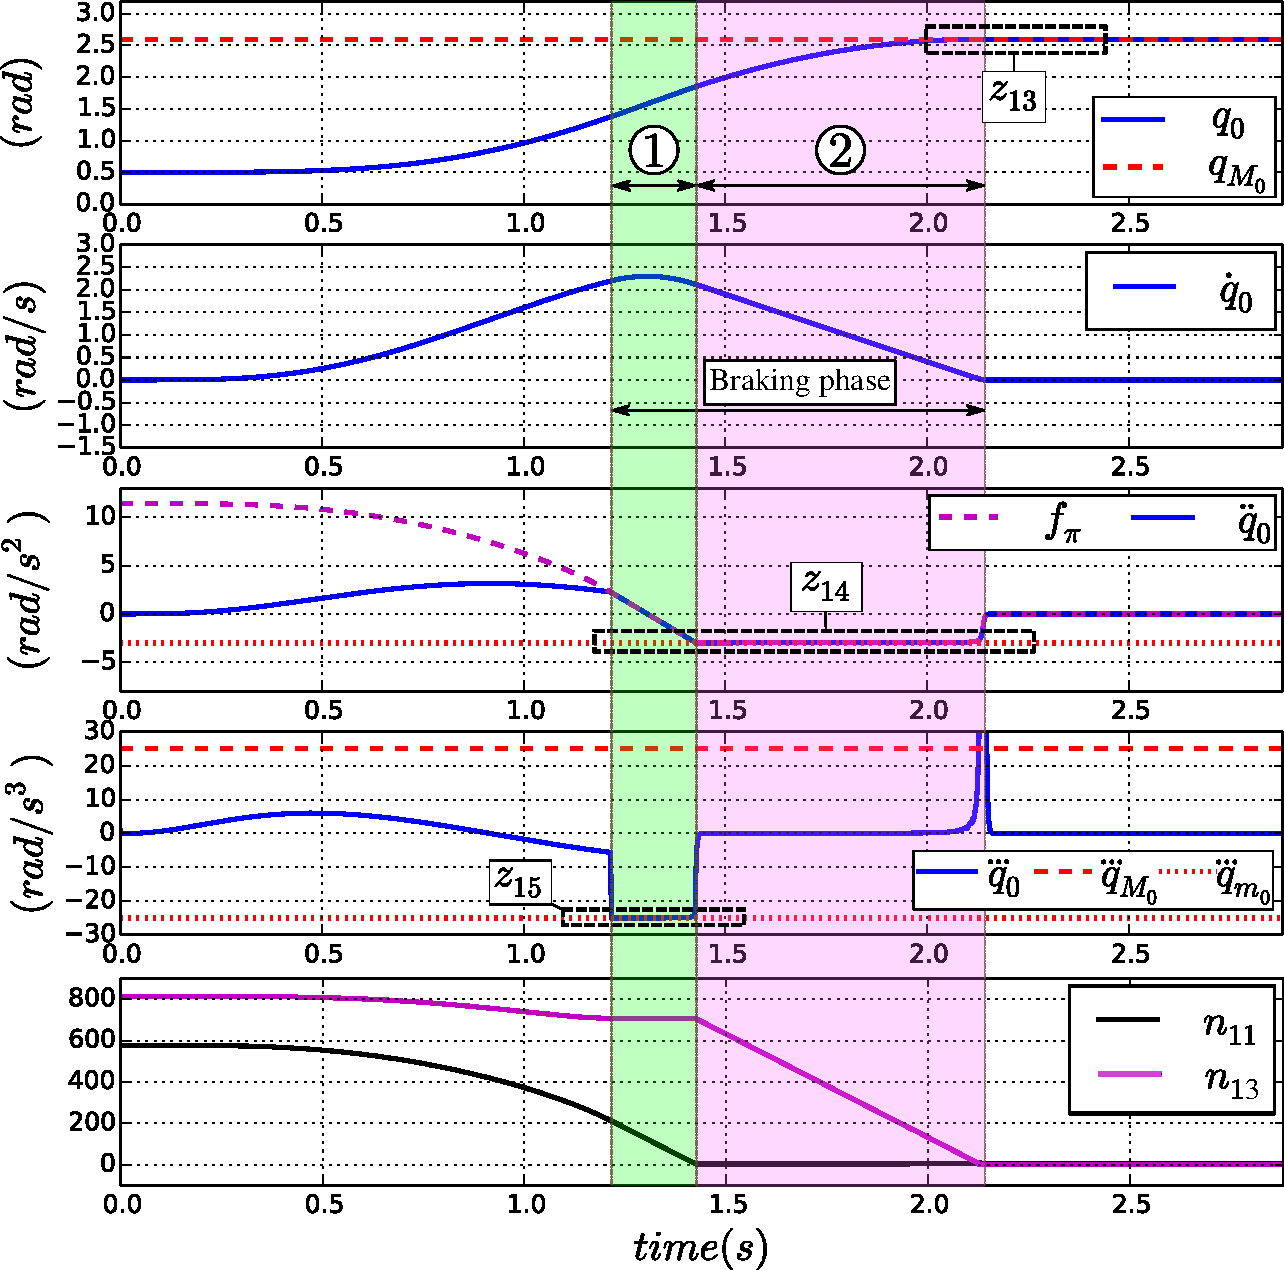
\includegraphics[width=0.8\columnwidth]{/home/anis/Desktop/THESIS_ANIS/THESIS/figures/Constrcomp/9_Posi_constr_jerk_acc_comp_non_complete_formula_3}}
%\caption{State $S$ of joint $0$ during the braking phase to cope with a maximum position limit $q_{M_{0}}$; The new constraint formulation (\ref{eq:Constr_comp_posi_acc_jerk_1_final}) that takes into account both deceleration and jerk capabilities $\dddot{q}_{m_{0}} = -25~rad.s^{-3}, \ddot{q}_{m_{0}}= -3~rad.s^{-2}$ is used. Top to bottom: position, velocity, acceleration, jerk and $(n_{11}, n_{13})$} 
%\label{fig:9_Posi_constr_jerk_acc_comp_non_complete_formula_3}
%\end{figure}
%\begin{figure}[!htbp]
%\centering
%{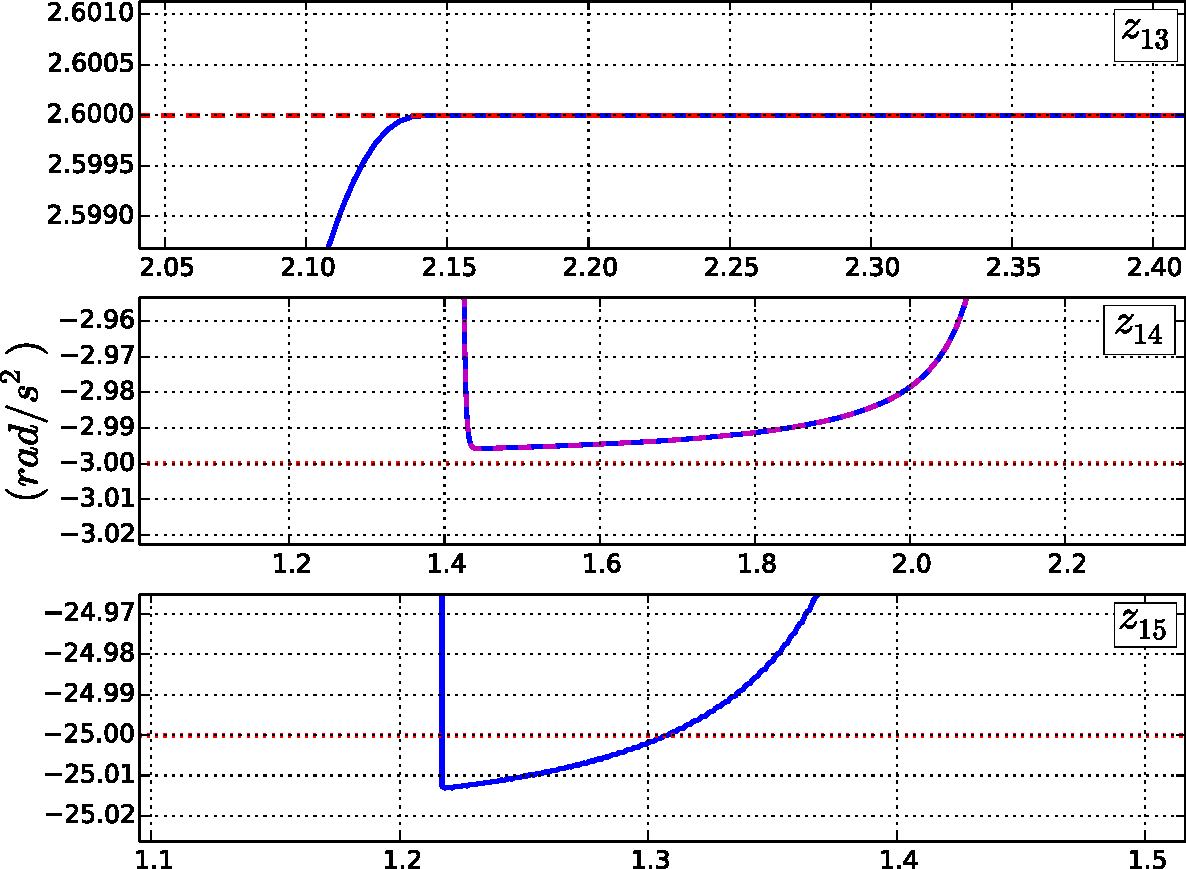
\includegraphics[width=0.8\columnwidth]{/home/anis/Desktop/THESIS_ANIS/THESIS/figures/Constrcomp/9_Posi_constr_jerk_acc_comp_non_complete_formula_3_zoom}}
%\caption{Zooms corresponding to Fig.~\ref{fig:9_Posi_constr_jerk_acc_comp_non_complete_formula_3}.} 
%\label{fig:9_Posi_constr_jerk_acc_comp_non_complete_formula_3_zoom}
%\end{figure}
\begin{figure}[!htbp]
\centering
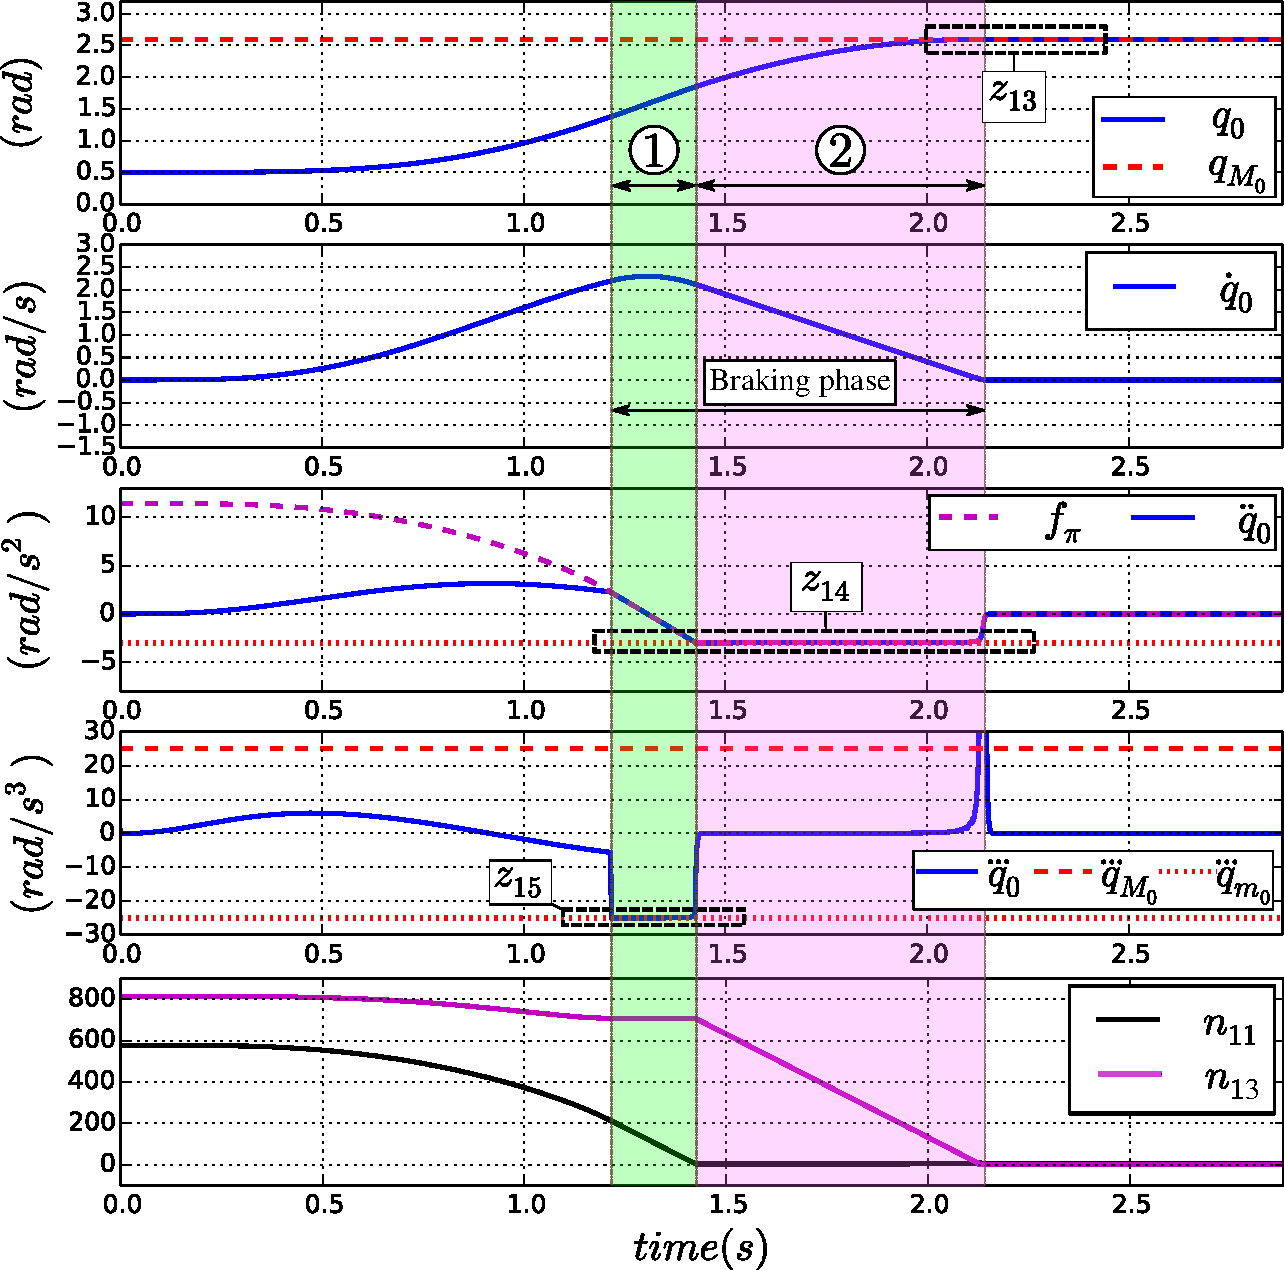
\includegraphics[width=0.92\columnwidth]{/home/anis/Desktop/THESIS_ANIS/THESIS/figures/Constrcomp/9_Posi_constr_jerk_acc_comp_non_complete_formula_3}
\caption{Extended state $S$ of joint $0$ during a \textit{non-complete} braking phase implicitly induced to cope with an upper position limit $q_{M_{0}}$. The new formulation of the constraint on articular position (\ref{eq:Constr_comp_posi_acc_jerk_1_final}), that takes into account both the articular jerk and deceleration capabilities $(\dddot{q}_{m_{0}} = -25~rad.s^{-3})$, $(\ddot{q}_{m_{0}}= -3~rad.s^{-2})$ is used. Top to bottom: position, velocity, acceleration, jerk and $(n_{11}, n_{13})$. See $z_{13}$ and $z_{14}$ in Fig.~\ref{fig:9_Posi_constr_jerk_acc_comp_non_complete_formula_3_zoom}.} 
\label{fig:9_Posi_constr_jerk_acc_comp_non_complete_formula_3}
\end{figure}
\begin{figure}[!htbp]
\centering
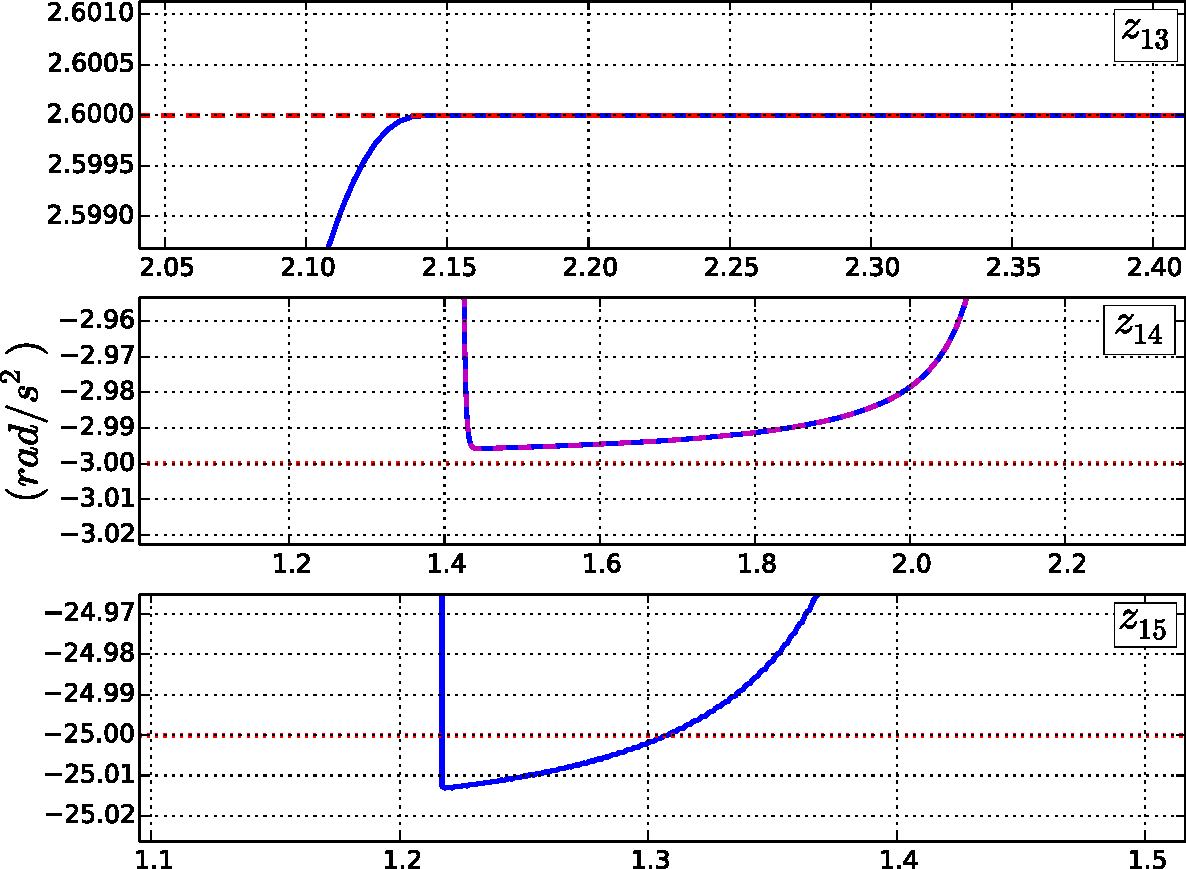
\includegraphics[width=0.90\columnwidth]{/home/anis/Desktop/THESIS_ANIS/THESIS/figures/Constrcomp/9_Posi_constr_jerk_acc_comp_non_complete_formula_3_zoom}
\caption{Zooms corresponding to Fig.~\ref{fig:9_Posi_constr_jerk_acc_comp_non_complete_formula_3}.} 
\label{fig:9_Posi_constr_jerk_acc_comp_non_complete_formula_3_zoom}
\end{figure}
%
%\begin{landscape}
%\begin{figure}
%\begin{minipage}[c]{0.5\linewidth}
%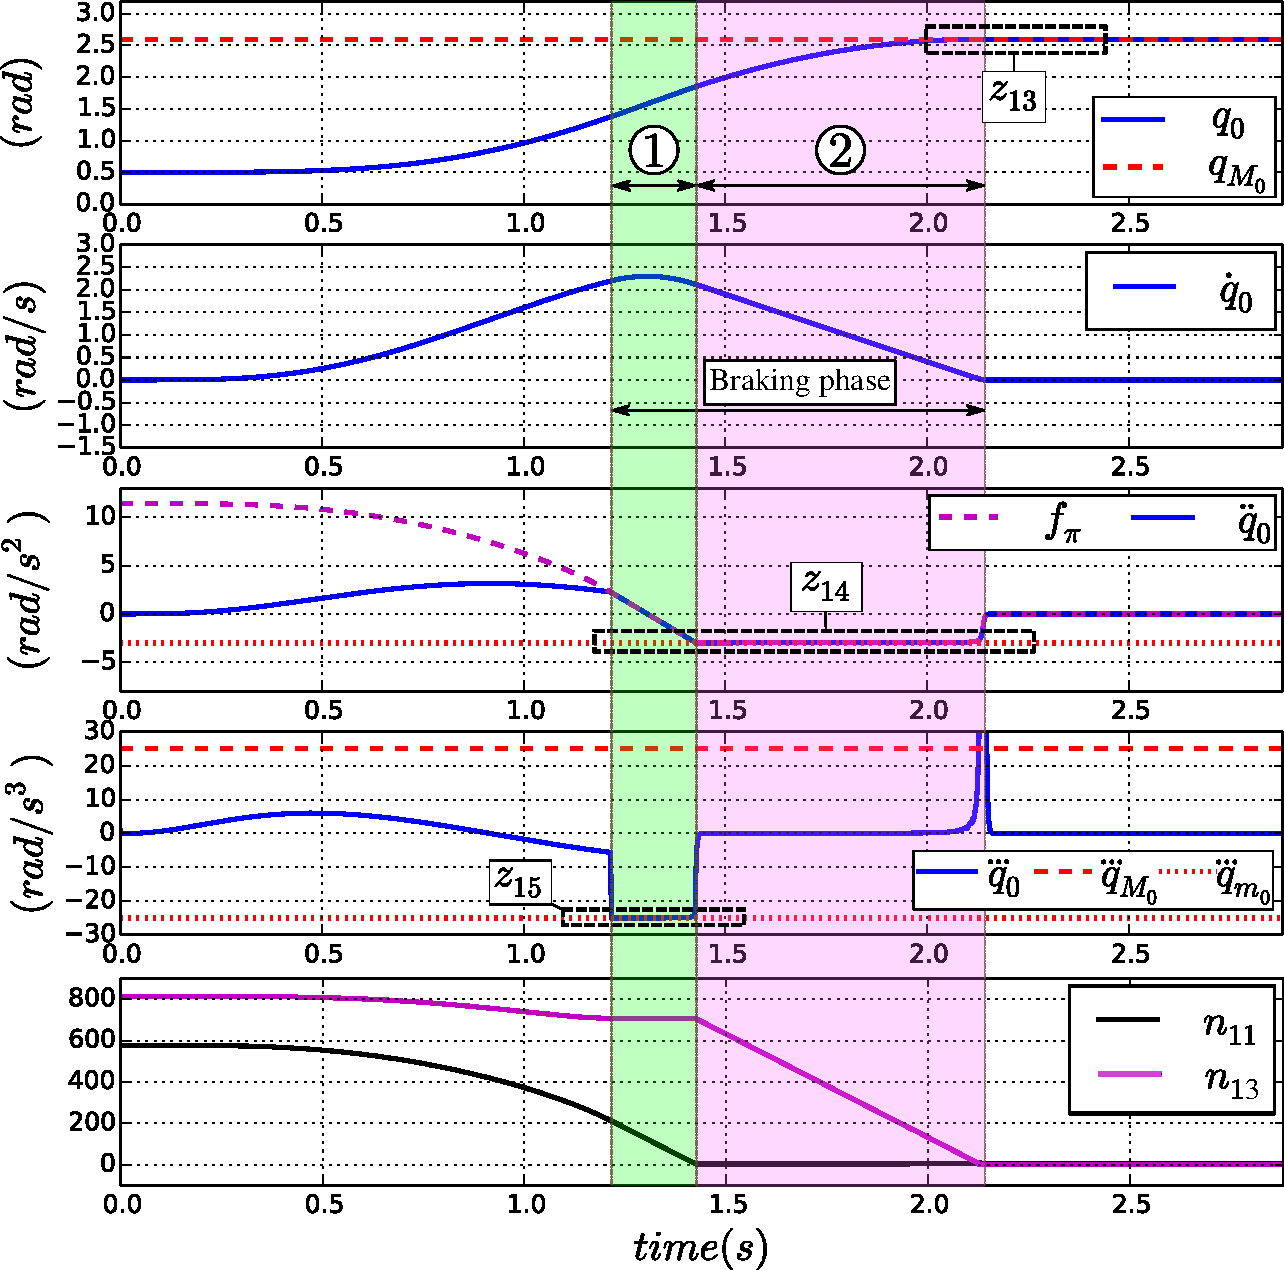
\includegraphics[width=0.99\columnwidth]{/home/anis/Desktop/THESIS_ANIS/THESIS/figures/Constrcomp/9_Posi_constr_jerk_acc_comp_non_complete_formula_3}
%\caption{Extended state $S$ of joint $0$ during a \textit{non-complete} braking phase implicitly induced to cope with an upper position limit $q_{M_{0}}$. The new formulation of the constraint on articular position (\ref{eq:Constr_comp_posi_acc_jerk_1_final}), that takes into account both the articular jerk and deceleration capabilities $(\dddot{q}_{m_{0}} = -25~rad.s^{-3})$, $(\ddot{q}_{m_{0}}= -3~rad.s^{-2})$ is used. Top to bottom: position, velocity, acceleration, jerk and $(n_{11}, n_{13})$} 
%\label{fig:9_Posi_constr_jerk_acc_comp_non_complete_formula_3}
%\end{minipage}
%\hfill
%\begin{minipage}[c]{0.5\linewidth}
%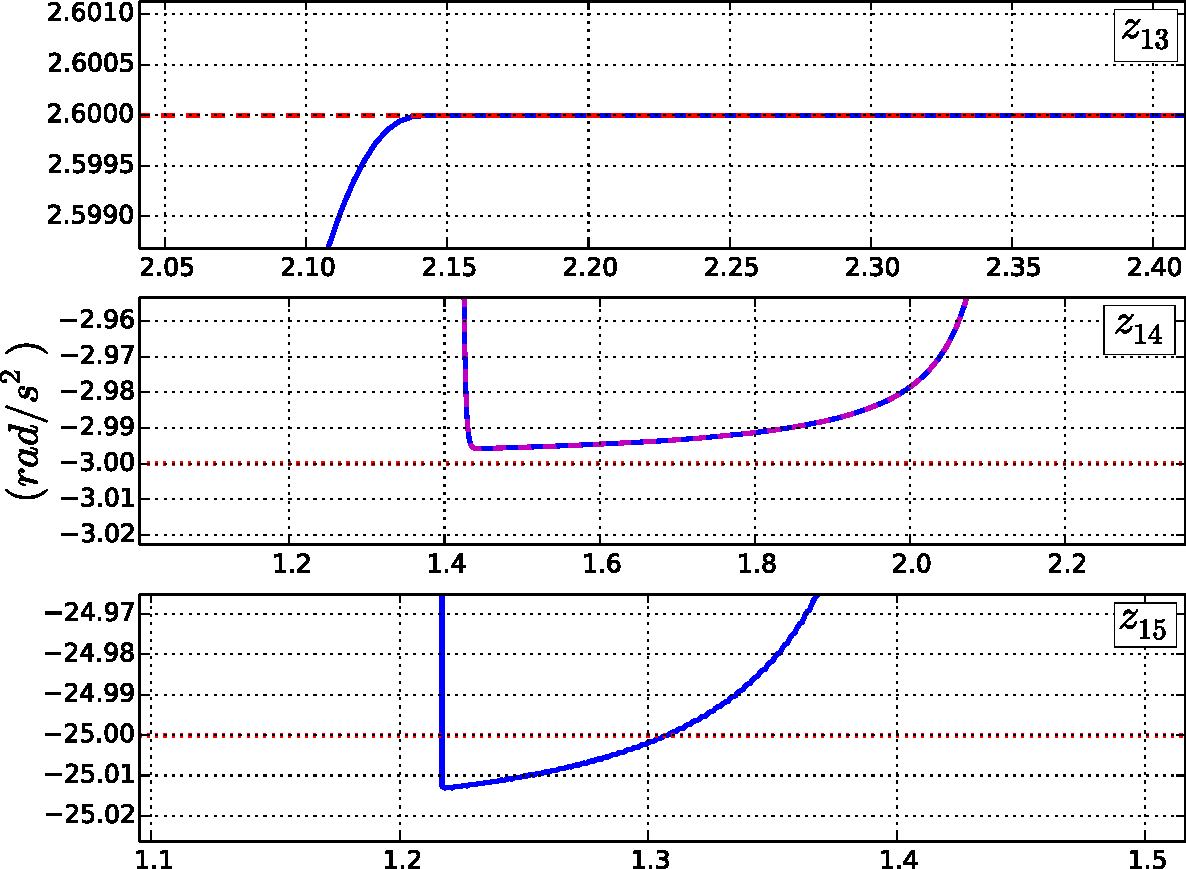
\includegraphics[width=0.90\columnwidth]{/home/anis/Desktop/THESIS_ANIS/THESIS/figures/Constrcomp/9_Posi_constr_jerk_acc_comp_non_complete_formula_3_zoom}
%\caption{Zooms corresponding to Fig.~\ref{fig:9_Posi_constr_jerk_acc_comp_non_complete_formula_3}.} 
%\label{fig:9_Posi_constr_jerk_acc_comp_non_complete_formula_3_zoom}
%\end{minipage}%
%\end{figure}
%\end{landscape}
%%%%%%%%%%%%%%%%%%%%%%%%%%SUBSUBSECTION%%%%%%%%%%%%%%%%%%%%%%%%%%%%%
%%%%%%%%%%%%%%%%%%%%%%%%%%SUBSUBSECTION%%%%%%%%%%%%%%%%%%%%%%%%%%%%%
\subsubsection{Joint position constraint incompatibility with both jerk and deceleration limits 2}
\label{subsec:case5}
Finally, the fully \nameref{label:complete} description of the braking phase is used to derive the \textit{proper} and complete formulation of the constraint on articular position. When coping with an upper position limit $q_M$, such braking phase is as follows: 1) the joint starts jerking with maximum negative jerk $\dddot{q}_{m}$ for $n_{15}$ iterations until maximum producible articular deceleration $\ddot{q}_m$ is reached. 2) This deceleration is then applied for $n_{17}$ control time-steps then, 3) ``\textit{de-charged}'' during $n_{19}$ iterations by jerking positively with maximum producible jerk $\dddot{q}_M$ (see Fig.~\ref{fig:per_Pr_jerk_ala_3}). The extended state \textit{S} of the system during this \nameref{label:complete} braking phase can be described as:  
\clearpage
\begin{equation} 
\resizebox{0.89\hsize}{!}{$
\begin{split}
\left.\begin{aligned}
\textit{S}_{|k+1}&\left\{\begin{array}{lcl}
q_{|k+1} \hspace{17mm}= q_{|k} + \dot{q}_{|k} \delta t, \\
\dot{q}_{|k+1} \hspace{17mm}= \dot{q}_{|k} + \ddot{q}_{|k} \delta t, \\
\ddot{q}_{|k+1} \hspace{17mm}= \ddot{q}_{|k} + \dddot{q}_{m} \delta t;
\end{array}\right. \\
&\hspace{7mm}\vdots\ \hspace{28mm}\vdots\ \\
\textit{S}_{|k+n_{15}}&\left\{\begin{array}{lcl}
q_{|k+n_{15}} \hspace{14mm}= q_{|k+n_{15}-1} + \dot{q}_{|k+n_{15}-1} \delta t, \\
\dot{q}_{|k+n_{15}} \hspace{14mm}= \dot{q}_{|k+n_{15}-1} + \ddot{q}_{|k+n_{15}-1} \delta t, \\
\ddot{q}_{|k+n_{15}} \hspace{14mm}= \ddot{q}_{|k+n_{15}-1} + \dddot{q}_{m} \delta t;
\end{array}\right.
\end{aligned}  \hspace{26mm}\right\}\textnormal{Equivalent to (\ref{eq:discretized_dynamics_posi_jerk_braking})}  \\[0.5cm]
\left.\begin{aligned}
\textit{S}_{|k+n_{15}+1}&\left\{\begin{array}{lcl}
q_{|k+n_{15}+1}  \hspace{10mm}= q_{|k+n_{15}} + \dot{q}_{|k+n_{15}} \delta t, \\
\dot{q}_{|k+n_{15}+1}  \hspace{10mm}= \dot{q}_{|k+n_{15}} + \ddot{q}_{m} \delta t; \\
\end{array}\right.\\
&\hspace{7mm}\vdots\ \hspace{28mm}\vdots\ \\
\textit{S}_{|k+n_{15}+n_{17}}&\left\{\begin{array}{lcl}
q_{|k+n_{15}+n_{17}} \hspace{7mm}= q_{|k+n_{15}+n_{17}-1} + \dot{q}_{|k+n_{15}+n_{17}-1} \delta t, \\
\dot{q}_{|k+n_{15}+n_{17}} \hspace{7mm}= \dot{q}_{|k+n_{15}+n_{17}-1} + \ddot{q}_{m} \delta t; \\
\end{array}\right. 
\end{aligned} \hspace{13mm}\right\}\textnormal{Equivalent to (\ref{eq:discretized_dynamics_posi_decel})}  \\[0.5cm]
\left.\begin{aligned}
\textit{S}_{|k+n_{15}+n_{17}+1}&\left\{\begin{array}{lcl}
q_{|k+n_{15}+n_{17}+1} \hspace{3mm}= q_{|k+n_{15}+n_{17}} + \dot{q}_{|k+n_{15}+n_{17}} \delta t, \\
\dot{q}_{|k+n_{15}+n_{17}+1} \hspace{3mm}= \dot{q}_{|k+n_{15}+n_{17}} + \ddot{q}_{|k+n_{15}+n_{17}} \delta t, \\
\ddot{q}_{|k+n_{15}+n_{17}+1}  \hspace{3mm}= \ddot{q}_{|k+n_{15}+n_{17}} + \dddot{q}_{M} \delta t;
\end{array}\right.\\
&\hspace{7mm}\vdots\ \hspace{29mm}\vdots\ \\
\textit{S}_{|k+n_{15}+n_{17}+n_{19}}&\left\{\begin{array}{lcl}
q_{|k+n_{15}+n_{17}+n_{19}} = q_{|k+n_{15}+n_{17}+n_{19}-1} + \dot{q}_{|k+n_{15}+n_{17}+n_{19}-1} \delta t, \\
\dot{q}_{|k+n_{15}+n_{17}+n_{19}} = \dot{q}_{|k+n_{15}+n_{17}+n_{19}-1} + \ddot{q}_{|k+n_{15}+n_{17}+n_{19}-1} \delta t, \\
\ddot{q}_{|k+n_{15}+n_{17}+n_{19}} = \ddot{q}_{|k+n_{15}+n_{17}+n_{19}-1} + \dddot{q}_{M} \delta t.
\end{array}\right.
\end{aligned}\right\}\textnormal{Equivalent to (\ref{eq:discretized_dynamics_posi_jerk_braking})} 
\end{split}$}
\label{eq:S_with_const_qdddot_m_const_qddot_m_const_qdddot_M}
\end{equation} 
The evolution of the joint's articular position in $(n_{15}+n_{17}+n_{19})$ iterations is equal to the general form\footnote{Computed using Maple \cite{maple}.} of the numerical sequence  (\ref{eq:S_with_const_qdddot_m_const_qddot_m_const_qdddot_M}):
\begin{equation}
\begin{split}
q_{|k+n_{15}+n_{17}+n_{19}} = &q_{|k+n_{15} + n_{17}} + n_{19} \dot{q}_{|k+n_{15}+n_{17}} \delta t \\
&+ \frac{\left(n_{19}^{2}-n_{19}\right)}{2} \ddot{q}_{|k+n_{15}+n_{17}} \delta t^{2} \\
&+ \left(\frac{n_{19}^{3}}{6}-\frac{n_{19}^{2}}{2}+\frac{n_{19}}{3}\right) \dddot{q}_{M} \delta t^{3},
\end{split}
\label{eq:q_evolution_with_const_qdddot_m_const_qddot_m_const_qdddot_M}
\end{equation} 
with: \\
\begin{equation}
\left\{\begin{array}{lcl}
q_{|k+n_{15}+n_{17}} = q_{|k+n_{15}} + n_{17}  \dot{q}_{|k+n_{15}} \delta t + \frac{\left(n_{17}^{2}-n_{17}\right)}{2} \ddot{q}_{m} \delta t^{2}, \\
\hspace{20mm}= q_{|k} + \left(n_{15}+n_{17}\right) \dot{q}_{|k} \delta t + \left[\left(n_{15} n_{17}\right)+\frac{\left(n_{15}^2-n_{15}\right)}{2}\right] \ddot{q}_{|k} \delta t^2 \\
\hspace{24mm}+ \frac{\left(n_{17}^2-n_{17}\right)}{2} \ddot{q}_{m} \delta t^2 \\
\hspace{24mm}+ \left[\frac{n_{17}\left(n_{15}^2-n_{15}\right)}{2}+\left(\frac{n_{15}^3}{6}-\frac{n_{15}^2}{2}+\frac{n_{15}}{3}\right)\right] \dddot{q}_{m} \delta t^3, \\
\dot{q}_{|k+n_{15}+n_{17}} = \dot{q}_{|k+n_{15}} + n_{17} \ddot{q}_{m} \delta t, \\
\hspace{20mm}= \dot{q}_{|k} + n_{15} \ddot{q}_{|k} \deta t + \frac{\left(n_{15}^{2}-n_{15}\right)}{2} \dddot{q}_{m} \delta t^{2} + n_{17} \ddot{q}_{m} \delta t, \\
\ddot{q}_{|k+n_{15}+n_{17}} \hspace{1mm}= \ddot{q}_{|k} + \dddot{q}_{m} \delta t. 
\end{array}\right. 
\end{equation}
$q_{|k+n_{15}}$, $q_{|k+n_{15}+n_{17}}$ and $\dot{q}_{|k+n_{15}}$ are respectively equivalent to  (\ref{eq:q_evolution_with_const_qdddot_m}), (\ref{eq:q_evolution_with_const_qddot_m_and_qdddot_m_2_final}) and (\ref{eq:q_dot_evolution_with_const_qdddot_m}). When developed, (\ref{eq:q_evolution_with_const_qdddot_m_const_qddot_m_const_qdddot_M}) becomes:
\begin{equation}
\begin{split}
q_{|k+n_{15}+n_{17}+n_{19}} =\hspace{1mm}&q_{|k} + \left(n_{15}+n_{17}+n_{19}\right) \dot{q}_{|k} \delta t \\
&+ \left[n_{15}\left(n_{17}+n_{19}\right)+\frac{\left(n_{15}^2-n_{15}\right)+\left(n_{19}^2-n_{19}\right)}{2}]\ddot{q}_{|k} \delta t^2 \\
&+ \left[\frac{\left(n_{17}+n_{19}\right)+\left(n_{15}^2-n_{15}\right)}{2}+\left(\frac{n_{15}^3}{6}-\frac{n_{15}^2}{2}+\frac{n_{15}}{3}\right)\right]\dddot{q}_{m} \delta t^3 \\
&+ \left[\left(n_{17} n_{19}\right)+\frac{\left(n_{17}^2-n_{17}\right)+\left(n_{19}^2-n_{19}\right)}{2}\right] \ddot{q}_{m} \delta t^2 \\
&+ \left(\frac{n_{19}^3}{6}-\frac{n_{19}^2}{2}+\frac{n_{19}}{3}\right)\dddot{q}_{M} \delta t^3.
\end{split}
\label{eq:q_evolution_with_const_qdddot_m_const_qddot_m_const_qdddot_M_dev}
\end{equation} 
With: $q_{|k} \geq 0$, $\dot{q}_{|k} \geq 0$ , $\dddot{q}_m \leq 0$, $\ddot{q}_m \leq 0$ and $\dddot{q}_M \geq 0$. The condition $q_{|k+n_{15}+n_{17}+n_{19}} \leq q_M$ for all integers $(n_{15}$, $n_{17}$, $n_{19})$ leads to:
\begin{equation}
\begin{split}
\ddot{q}_{|k}^{c} \leq &\frac{\left(q_{M}-q_{|k}\right)}{\left[n_{15}\left(n_{17}+n_{19}\right)+\frac{\left(n_{15}^2-n_{15}\right)+\left(n_{19}^2-n_{19}\right)}{2}\right]\delta t^2} \\
&- \frac{\left(n_{15}+n_{17}+n_{19}\right)\dot{q}_{|k}}{\left[n_{15}\left(n_{17}+n_{19}\right)+\frac{\left(n_{15}^2-n_{15}\right)+\left(n_{19}^2-n_{19}\right)}{2}\right]\delta t} \\
&- \frac{\left[\frac{\left(n_{17}+n_{19}\right)+\left(n_{15}^2-n_{15}\right)}{2}+\left(\frac{n_{15}^3}{6}-\frac{n_{15}^2}{2}+\frac{n_{15}}{3}\right)\right]\dddot{q}_{m} \delta t}{\left[n_{15}\left(n_{17}+n_{19}\right)+\frac{\left(n_{15}^2-n_{15}\right)+\left(n_{19}^2-n_{19}\right)}{2}\right]} \\
&- \frac{\left[\left(n_{17} n_{19}\right)+\frac{\left(n_{17}^2-n_{17}\right)+\left(n_{19}^2-n_{19}\right)}{2}\right]\ddot{q}_{m}}{\left[n_{15}\left(n_{17}+n_{19}\right)+\frac{\left(n_{15}^2-n_{15}\right)+\left(n_{19}^2-n_{19}\right)}{2}\right]} \\
&- \frac{\left[\left(\frac{n_{19}^3}{6}-\frac{n_{19}^2}{2}+\frac{n_{19}}{3}\right)\right]\dddot{q}_{M} \delta t}{\left[n_{15}\left(n_{17}+n_{19}\right)+\frac{\left(n_{15}^2-n_{15}\right)+\left(n_{19}^2-n_{19}\right)}{2}\right]}.
\end{split}
\label{eq:q_ddot_posi_acc_jerk_comp_complete_1}
\end{equation} 
$(n_{15}$, $n_{17}$, $n_{19})$ are the integers minimizing the right-hand side of (\ref{eq:q_ddot_posi_acc_jerk_comp_complete_1}).
Following the same reasoning for the lower position limit, the condition $q_{|k+n_{16}+n_{18}+n_{20}} \geq q_{m}$ can be reflected on the acceleration control variable as follows:
\begin{equation}
\begin{split}
\ddot{q}_{|k}^{c} \geq &\frac{\left(q_{m}-q_{|k}\right)}{\left[n_{16}\left(n_{18}+n_{20}\right)+\frac{\left(n_{16}^2-n_{16}\right)+\left(n_{20}^2-n_{20}\right)}{2}\right]\delta t^2} \\
&- \frac{\left(n_{16}+n_{18}+n_{20}\right)\dot{q}_{|k}}{\left[n_{16}\left(n_{18}+n_{20}\right)+\frac{\left(n_{16}^2-n_{16}\right)+\left(n_{20}^2-n_{20}\right)}{2}\right]\delta t} \\
&- \frac{\left[\frac{\left(n_{18}+n_{20}\right)+\left(n_{16}^2-n_{16}\right)}{2}+\left(\frac{n_{16}^3}{6}-\frac{n_{16}^2}{2}+\frac{n_{16}}{3}\right)\right]\dddot{q}_{M} \delta t}{\left[n_{16}\left(n_{18}+n_{20}\right)+\frac{\left(n_{16}^2-n_{16}\right)+\left(n_{20}^2-n_{20}\right)}{2}\right]} \\
&- \frac{\left[\left(n_{18} n_{20}\right)+\frac{\left(n_{18}^2-n_{18}\right)+\left(n_{20}^2-n_{20}\right)}{2}\right]\ddot{q}_{M}}{\left[n_{16}\left(n_{18}+n_{20}\right)+\frac{\left(n_{16}^2-n_{16}\right)+\left(n_{20}^2-n_{20}\right)}{2}\right]} \\
&- \frac{\left(\frac{n_{20}^3}{6}-\frac{n_{20}^2}{2}+\frac{n_{20}}{3}\right)\dddot{q}_{m} \delta t}{\left[n_{16}\left(n_{18}+n_{20}\right)+\frac{\left(n_{16}^2-n_{16}\right)+\left(n_{20}^2-n_{20}\right)}{2}\right]},
\end{split}
\label{eq:q_ddot_posi_acc_jerk_comp_complete_2}
\end{equation} 
with $(n_{16}, n_{18}, n_{20})$: the integers maximizing the right-hand side of (\ref{eq:q_ddot_posi_acc_jerk_comp_complete_2}). \\
$\textit{f}_{\chi}$ and $\textit{f}_{\phi}$ are respectively equivalent to the right-hand sides of (\ref{eq:q_ddot_posi_acc_jerk_comp_complete_1}) and (\ref{eq:q_ddot_posi_acc_jerk_comp_complete_2}). \\
\noindent\begin{minipage}{\textwidth}
\renewcommand\footnoterule{}                  %% This line should come here.
\begin{algorithm}[H]
\caption{Compute $n_{15}, n_{16}, n_{17}, n_{18}, n_{19}, n_{20}, f_{\chi}$ and $f_{\phi}$}
\label{alg:compute_n_15_n_16_n_17_n_18_n_19_n_20_f_chi_f_phi}
\begin{algorithmic}[1]
%f_{\phi}(n_{16}, n_{18}, n_{20}) and f_{\chi}(n_{15}, n_{17}, n_{19})  
      % n1_pos  n2_pos  n3_pos             n1_neg  n2_neg  n3_neg
\Require $q_M, q_m, q_{|k}, \dot{q}_{|k}, \ddot{q}_{M},\ddot{q}_{m},\dddot{q}_{M},\dddot{q}_{m}, \delta t$
\State{$f_{{\chi}_{max}} \hspace{0.5mm} \gets \ddot{q}_{m} \qquad f_{{\phi}_{min}} \hspace{0.5mm} \gets \ddot{q}_{M}$}
%\myState{$f_{{\chi}_{max}} \hspace{0.5mm} \gets \ddot{q}_{m}$}
%\myState{$f_{{\phi}_{min}} \hspace{0.5mm} \gets \ddot{q}_{M}$} 
\For{($i_1 = 1 \rightarrow N_1$)}
\State{$n_{16}^{*} \gets i_1 \qquad n_{15}^{*} \gets i_1$}
%\myState{$n_{16}^{*} \gets i_1$}
%\myState{$n_{15}^{*} \gets i_1$}
\For{($i_2 = 0 \rightarrow N_2$)}
\State{$n_{18}^{*} \gets i_2 \qquad n_{17}^{*} \gets i_2$}
%\myState{$n_{18}^{*} \gets i_2$}
%\myState{$n_{17}^{*} \gets i_2$}
        \If{($\ddot{q}_{|k} \geq 0$)} 
             \State{$n_{{20}_{\mathbb{R}^{+}}}^{*} \gets n_{16}-\abs[\Big]{\myfrac[5pt]{\ddot{q}_{|k}}{\dddot{q}_m \delta t}} \qquad n_{{19}_{\mathbb{R}^{+}}}^{*} \gets n_{15}+\abs[\Big]{\myfrac[5pt]{\ddot{q}_{|k}}{\dddot{q}_M \delta t}}$}
%             \myState{$n_{20}^{*} \gets n_{16}-\abs[\Big]{\myfrac[5pt]{\ddot{q}_{|k}}{\dddot{q}_m \delta t}}$}
%             \myState{$n_{19}^{*} \gets n_{15}+\abs[\Big]{\myfrac[5pt]{\ddot{q}_{|k}}{\dddot{q}_M \delta t}}$}
        \EndIf 
        \If{($\ddot{q}_{|k} < 0$)} 
             \State{$n_{{20}_{\mathbb{R}^{+}}}^{*} \gets n_{16}+\abs[\Big]{\myfrac[5pt]{\ddot{q}_{|k}}{\dddot{q}_M \delta t}} \qquad n_{{19}_{\mathbb{R}^{+}}}^{*} \gets n_{15}-\abs[\Big]{\myfrac[5pt]{\ddot{q}_{|k}}{\dddot{q}_m \delta t}}$}
%             \myState{$n_{20}^{*} \gets n_{16}+\abs[\Big]{\myfrac[5pt]{\ddot{q}_{|k}}{\dddot{q}_M \delta t}}$}
%             \myState{$n_{19}^{*} \gets n_{15}-\abs[\Big]{\myfrac[5pt]{\ddot{q}_{|k}}{\dddot{q}_m \delta t}}$}
%        \If{($n_{15}^{*} \leq 1$)}
%             \myState{$n_{20}^{*} \gets \abs[\Big]{\myfrac[5pt]{\ddot{q}_{|k}}{\dddot{q}_M \delta t}}$}
%        \EndIf
        \IfThenElse{($n_{16}^{*} \leq 1$)}% If ...
            {$n_{{20}_{\mathbb{R}^{+}}}^{*} \gets \abs[\Big]{\myfrac[5pt]{\ddot{q}_{|k}}{\dddot{q}_m \delta t}}$}% ...then... 
\vspace{1.5mm}             
%        \If{($n_{16}^{*} \leq 1$)}
%             \myState{$n_{19}^{*} \gets \abs[\Big]{\myfrac[5pt]{\ddot{q}_{|k}}{\dddot{q}_m \delta t}}$}
%        \EndIf
        \IfThenElse{($n_{15}^{*} \leq 1$)}% If ...
            {$n_{{19}_{\mathbb{R}^{+}}}^{*} \gets \abs[\Big]{\myfrac[5pt]{\ddot{q}_{|k}}{\dddot{q}_M \delta t}}$}% ...then...
        
        \EndIf
%f_{\phi}(n_{16}, n_{18}, n_{20}) and f_{\chi}(n_{15}, n_{17}, n_{19})  
      % n1_pos  n2_pos  n3_pos             n1_neg  n2_neg  n3_neg
\IfThenElse{($n_{15}^{*} \leq 1$)}% If ...
            {$n_{15}^{*} \gets 1$}% ...then...
\IfThenElse{($n_{16}^{*} \leq 1$)}% If ...
            {$n_{16}^{*} \gets 1$}% ...then...            
\IfThenElse{($n_{{19}_{\mathbb{R}^{+}}}^{*} \leq 2$)}% If ...
            {$n_{{19}_{\mathbb{R}^{+}}}^{*} \gets 2$}% ...then...
\IfThenElse{($n_{{20}_{\mathbb{R}^{+}}}^{*} \leq 2$)}% If ...
            {$n_{{20}_{\mathbb{R}^{+}}}^{*} \gets 2$}% ...then...      
\myState{$f_{\chi}^{*} \gets f_{\chi}(q_m, q_{|k}, \dot{q}_{|k}, \dddot{q}_M, \ddot{q}_M, \dddot{q}_m, n_{15}^{*}, n_{17}^{*}, n_{19}^{*})$}
\myState{$f_{\phi}^{*} \gets f_{\phi}(q_M, q_{|k}, \dot{q}_{|k}, \dddot{q}_m, \ddot{q}_m, \dddot{q}_M, n_{16}^{*}, n_{18}^{*}, n_{20}^{*})$}
\If{($f_{\chi}^{*} \geq f_{{\chi}_{max}}$)}
\State{$f_{{\chi}_{max}} \gets f_{\chi}^{*} \qquad n_{16} \gets n_{16}^{*} \qquad n_{18} \gets n_{18}^{*} \qquad n_{20}$\footnote{\label{note2} For stability in the computation of $f_{\chi}$ and $f_{\phi}$, ($n_{19}^{*}, n_{20}^{*}$) are used as real numbers (even if previously defined as numbers of iterations). The same for $n_{19}$ and $n_{20}$.} $\gets n_{{20}_{\mathbb{R}^{+}}}^{*}$}
%\myState{$f_{{\chi}_{max}} \gets f_{\chi}^{*}$}
%\myState{$n_{16} \gets n_{16}^{*}$}
%\myState{$n_{18} \gets n_{18}^{*}$}
%\myState{$n_{20} \gets n_{20}^{*}$}
\EndIf 
\If{($f_{\phi}^{*} \leq f_{{\phi}_{min}}$)}
\State{$f_{{\phi}_{min}} \gets f_{\phi}^{*} \qquad n_{15} \gets n_{15}^{*} \qquad n_{17} \gets n_{17}^{*} \qquad n_{19}\footnoteref{note2} \gets n_{{19}_{\mathbb{R}^{+}}}^{*}$}
%\myState{$f_{{\phi}_{min}} \gets f_{\phi}^{*}$}
%\myState{$n_{15} \gets n_{15}^{*}$}
%\myState{$n_{17} \gets n_{17}^{*}$}
%\myState{$n_{19} \gets n_{19}^{*}$}
\EndIf 
\EndFor
\EndFor
\State{$f_{{\chi}} \gets f_{{\chi}_{max}} \qquad f_{{\phi}} \gets f_{{\phi}_{min}}$}
%\myState{$f_{{\chi}} \gets f_{{\chi}_{max}}$}
%\myState{$f_{{\phi}} \gets f_{{\phi}_{min}}$}
\myState \Return{$n_{15}, n_{16}, n_{17}, n_{18}, n_{19}, n_{20}, f_{\chi}, f_{\phi}$}\;
\end{algorithmic}
\end{algorithm}
\end{minipage} \\
\\
$n_{15}, n_{16}, n_{17}, n_{18}, n_{19}, n_{20}, f_{\chi}$ and $f_{\phi}$ can be computed numerically as shown in Algorithm~\ref{alg:compute_n_15_n_16_n_17_n_18_n_19_n_20_f_chi_f_phi}. $N_1$ and $N_2$ in Algorithm~\ref{alg:compute_n_15_n_16_n_17_n_18_n_19_n_20_f_chi_f_phi} are fixed heuristically, they must however be $\geq$ to the number of iterations needed to perform the braking movement described in (\ref{eq:S_with_const_qdddot_m_const_qddot_m_const_qdddot_M}). More details on how to compute this parameter in Section~\ref{sec:concl_comp_cnstr}.
%********************************************************************%
\paragraph{Illustration 6}
For this simulation, the controller is implemented with the last \nameref{label:complete} formulation of the constraint on articular position (\ref{eq:q_ddot_posi_acc_jerk_comp_complete_1}), that takes into account both the positive and negative jerk capabilities, $[\dddot{q}_{m_{0}}, \dddot{q}_{M_{0}}] = [-25, 25]~rad.s^{-3}$ in addition to the deceleration capability $(\ddot{q}_{m_{0}} = -3~rad.s^{-2}$). As for the previous simulations, joint $0$ moves towards its upper position limit $q_{M_{0}}$.  The \textit{hard-coded} constraints on its articular acceleration (\ref{eq:cnt_lit_tme_step_3}) and articular jerk (\ref{eq:cnt_lit_tme_step_4}) are not considered in the configuration of the controller. 

Fig.~\ref{fig:11_Posi_constr_jerk_acc_comp_complete_formula_3}, illustrates the braking phase induced by the actuator of joint $0$ as it copes with its position limit $q_{M_{0}}$. the joint starts jerking negatively with maximum jerk $(\dddot{q} = \dddot{q}_{m_{0}})$  until maximum deceleration $\ddot{q}_{m_{0}}$ is reached (sub-phase \circled{1}). This deceleration is then used for several control time-steps (sub-phase \circled{2}) then ``\textit{de-charged}'' and brought to $0$ by jerking positively (sub-phase \circled{3}). By the end, joint $0$ is stopped exactly at its upper position limit $q_{M_{0}}$. The jerk profile in Fig.~\ref{fig:11_Posi_constr_jerk_acc_comp_complete_formula_3_zoom} shows an exceeding of $(0.013~rad.s^{-3})$ over the lower jerk limit $\dddot{q}_{m_{0}}$ and an other one of $(0.035~rad.s^{-2})$ over the lower deceleration limit $\ddot{q}_{m_{0}}$. As before, this is mainly due to the \textit{discrete} description of the braking phase that results into a \textit{discrete} formulation of the constraint on articular position. \\ 
Fig.~\ref{fig:10_Posi_constr_jerk_acc_comp_complete_formula_100} illustrates the induced braking phase in case the lower deceleration limit $\ddot{q}_{m_{0}}$ is fixed at $-100~rad.s^{-2}$. Consequently, the second braking \textit{sub-phase}\footnote{Considering an upper position limit, 3 sub-phases are distinguished during the \nameref{label:complete} braking phase: constant negative jerk, constant deceleration then constant positive jerk.} disappears resulting into an equivalent behaviour as for (\ref{eq:q_constr_on_q_ddot_with_const_qdddot_m_const_qdddot_M_1}) in Fig.~\ref{fig:8_Posi_constr_jerk_comp_25_complete_formula_no_backklash}.
%11
%\begin{figure}[!htbp]
%\centering
%{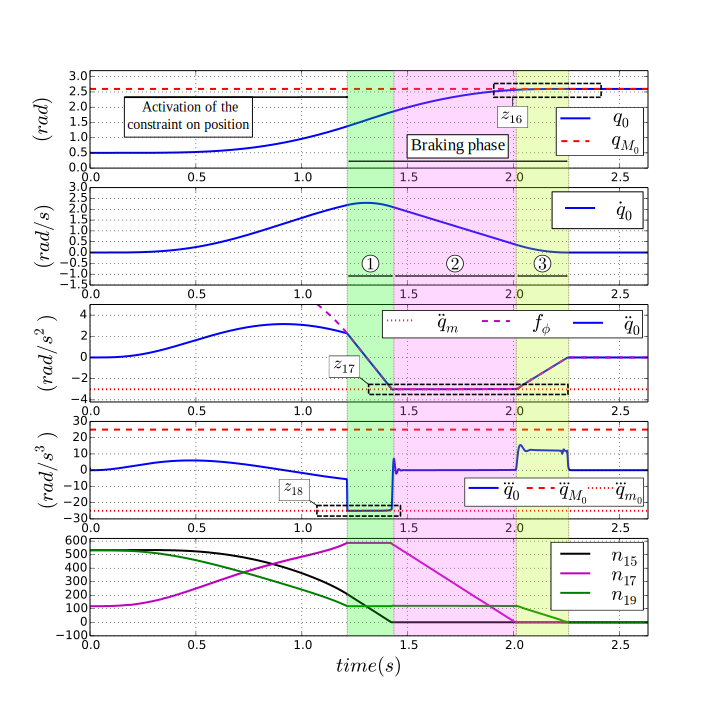
\includegraphics[width=0.8\columnwidth]{/home/anis/Desktop/THESIS_ANIS/THESIS/figures/Constrcomp/11_Posi_constr_jerk_acc_comp_complete_formula_3}}
%\caption{State $S$ of joint $0$ during the braking phase to cope with a maximum position limit $q_{M_{0}}$; The new constraint formulation (\ref{eq:q_ddot_posi_acc_jerk_comp_complete_1}) that takes into account the deceleration capability $\ddot{q}_{m_{0}}=-3~rad.s^{-2}$ in addition to the positive and negative jerk limits $[\dddot{q}_{m_{0}}, \dddot{q}_{M_{0}}] = [-25, 25]~rad.s^{-3}$ is used. Top to bottom: position, velocity, acceleration, jerk and $(n_{15}, n_{17}, n_{19})$.} 
%\label{fig:11_Posi_constr_jerk_acc_comp_complete_formula_3}
%\end{figure}
%\begin{figure}[!htbp]
%\centering
%{\includegraphics[width=0.8\columnwidth]{/home/anis/Desktop/THESIS_ANIS/THESIS/figures/Constrcomp/11_Posi_constr_jerk_acc_comp_complete_formula_3_zoom}}
%\caption{Zooms corresponding to Fig.~\ref{ref:11_Posi_constr_jerk_acc_comp_complete_formula_3}.} 
%\label{fig:11_Posi_constr_jerk_acc_comp_complete_formula_3_zoom}
%\end{figure}
%%10
%\begin{figure}[!htbp]
%\centering
%{\includegraphics[width=0.8\columnwidth]{/home/anis/Desktop/THESIS_ANIS/THESIS/figures/Constrcomp/10_Posi_constr_jerk_acc_comp_complete_formula_100}}
%\caption{State $S$ of joint $0$ during the braking phase to cope with a maximum position limit $q_{M_{0}}$; The new constraint formulation (\ref{eq:q_ddot_posi_acc_jerk_comp_complete_1}) that takes into account the deceleration capability $\ddot{q}_{m_{0}}=-100~rad.s^{-2}$ in addition to the positive and negative jerk limits $[\dddot{q}_{m_{0}}, \dddot{q}_{M_{0}}] = [-25, 25]~rad.s^{-3}$ is used. Top to bottom: position, velocity, acceleration, jerk and $(n_{15}, n_{17}, n_{19})$.} 
%\label{fig:10_Posi_constr_jerk_acc_comp_complete_formula_100}
%\end{figure}
%
\begin{figure}[!htbp]
\centering
\includegraphics[width=0.99\columnwidth]{/home/anis/Desktop/THESIS_ANIS/THESIS/figures/Constrcomp/11_Posi_constr_jerk_acc_comp_complete_formula_3}
\caption{Extended state $S$ of joint $0$ during the \textit{complete} braking phase to cope with an upper position limit $q_{M_{0}}$. The new formulation of the constraint on articular position (\ref{eq:q_ddot_posi_acc_jerk_comp_complete_1}), that takes into account the deceleration capability $\ddot{q}_{m_{0}}=-3~rad.s^{-2}$ in addition to the positive and negative jerk limits $[\dddot{q}_{m_{0}}, \dddot{q}_{M_{0}}] = [-25, 25]~rad.s^{-3}$ is used. Top to bottom: position, velocity, acceleration, jerk and $(n_{15}, n_{17}, n_{19})$. See $z_{16}$, $z_{17}$ and $z_{18}$ in Fig.~\ref{fig:11_Posi_constr_jerk_acc_comp_complete_formula_3_zoom}} 
\label{fig:11_Posi_constr_jerk_acc_comp_complete_formula_3}
\end{figure}
\begin{figure}[!htbp]
\centering
\includegraphics[width=0.90\columnwidth]{/home/anis/Desktop/THESIS_ANIS/THESIS/figures/Constrcomp/11_Posi_constr_jerk_acc_comp_complete_formula_3_zoom}
\caption{Zooms corresponding to Fig.~\ref{fig:11_Posi_constr_jerk_acc_comp_complete_formula_3}.} 
\label{fig:11_Posi_constr_jerk_acc_comp_complete_formula_3_zoom}
\end{figure}
%
%
%%11
%\begin{landscape}
%\begin{figure}
%\begin{minipage}[c]{0.5\linewidth}
%\includegraphics[width=0.99\columnwidth]{/home/anis/Desktop/THESIS_ANIS/THESIS/figures/Constrcomp/11_Posi_constr_jerk_acc_comp_complete_formula_3}
%\caption{Extended state $S$ of joint $0$ during the \textit{complete} braking phase to cope with an upper position limit $q_{M_{0}}$. The new formulation of the constraint on articular position (\ref{eq:q_ddot_posi_acc_jerk_comp_complete_1}), that takes into account the deceleration capability $\ddot{q}_{m_{0}}=-3~rad.s^{-2}$ in addition to the positive and negative jerk limits $[\dddot{q}_{m_{0}}, \dddot{q}_{M_{0}}] = [-25, 25]~rad.s^{-3}$ is used. Top to bottom: position, velocity, acceleration, jerk and $(n_{15}, n_{17}, n_{19})$.} 
%\label{fig:11_Posi_constr_jerk_acc_comp_complete_formula_3}
%\end{minipage}
%\hfill
%\begin{minipage}[c]{0.5\linewidth}
%\includegraphics[width=0.90\columnwidth]{/home/anis/Desktop/THESIS_ANIS/THESIS/figures/Constrcomp/11_Posi_constr_jerk_acc_comp_complete_formula_3_zoom}
%\caption{Zooms corresponding to Fig.~\ref{fig:11_Posi_constr_jerk_acc_comp_complete_formula_3}.} 
%\label{fig:11_Posi_constr_jerk_acc_comp_complete_formula_3_zoom}
%\end{minipage}%
%\end{figure}
%\end{landscape}
%10
\begin{figure}[!htbp]
\centering
{\includegraphics[width=0.99\columnwidth]{/home/anis/Desktop/THESIS_ANIS/THESIS/figures/Constrcomp/10_Posi_constr_jerk_acc_comp_complete_formula_100}}
\caption{State $S$ of joint $0$ during the braking phase to cope with an upper position limit $q_{M_{0}}$; The new constraint formulation (\ref{eq:q_ddot_posi_acc_jerk_comp_complete_1}) that takes into account the deceleration capability $\ddot{q}_{m_{0}}=-100~rad.s^{-2}$ in addition to the positive and negative jerk limits $[\dddot{q}_{m_{0}}, \dddot{q}_{M_{0}}] = [-25, 25]~rad.s^{-3}$ is used. Top to bottom: position, velocity, acceleration, jerk and $(n_{15}, n_{17}, n_{19})$.} 
\label{fig:10_Posi_constr_jerk_acc_comp_complete_formula_100}
\end{figure}
%%%%%%%%%%%%%%%%%%%%%%%%%%%%%%%%%%%%%%%%%%%%%%%%%%%%%%%%%
  %Final bounds on the acceleration control variable%
%%%%%%%%%%%%%%%%%%%%%%%%%%%%%%%%%%%%%%%%%%%%%%%%%%%%%%%%%                         
\section{Final bounds on the acceleration control variable}
\label{sec:finalb}
In this section, the final upper and lower bounds $[f_{\psi}, f_{\omega}]$ on the acceleration control variable $\ddot{q}_{|k}^{c}$ that allow a joint to cope with all the  constraints corresponding to its position, velocity, acceleration and jerk limitations at the same time are computed. Using the following algorithm: \\
\noindent\begin{minipage}{\textwidth}
\renewcommand\footnoterule{} 
\begin{algorithm}[H]
\caption{Compute $f_{\psi}$ and $f_{\omega}$}
\label{alg:compute_f_psi_f_omega}
\begin{algorithmic}[1]
%f_{\phi}(n_{16}, n_{18}, n_{20}) and f_{\chi}(n_{15}, n_{17}, n_{19})  
      % n1_pos  n2_pos  n3_pos             n1_neg  n2_neg  n3_neg
\Require $f_{\alpha}, f_{\beta}, f_{\lambda}, f_{\mu}, \ddot{q}_{M},\ddot{q}_{m}, \dddot{q}_{M},\dddot{q}_{m}, \delta t$
\State{$f_{\psi} \gets \ddot{q}_{M}$}
\State{$f_{\omega} \gets \ddot{q}_{m}$}
\State{$f_{\psi}^{*} \gets min(f_{\alpha}(\dot{q}_M, \dddot{q}_m),  f_{\lambda}(q_M, \dddot{q}_m, \ddot{q}_m, \dddot{q}_M), \ddot{q}_M, (\ddot{q}_{|k}+\dddot{q}_{M} \delta t))$}
\State{$f_{\omega}^{*} \gets max(f_{\beta}(\dot{q}_m, \dddot{q}_M),  f_{\mu}(q_m, \dddot{q}_M, \ddot{q}_M, \dddot{q}_m,), \ddot{q}_m, (\ddot{q}_{|k}+\dddot{q}_{m} \delta t))$}
\If{($\abs{f_{\psi}^{*} - \ddot{q}_{|k}^{c}} \leq \epsilon$\footnote{\label{note1}  e.g., $\epsilon = 1$})} 
     \State{$ f_{\psi} \gets f_{\psi}^{*}$}
\EndIf
\If{($\abs{f_{\omega}^{*} - \ddot{q}_{|k}^{c}} \leq \epsilon$)} 
     \State{$ f_{\omega} \gets f_{\omega}^{*}$}
\EndIf
\myState \Return{$f_{\psi}, f_{\omega}$}\;
\end{algorithmic}
\end{algorithm}
\end{minipage} \\
\\
The final constraint on the acceleration control variable $\ddot{q}_{|k}^{c}$ is written:
\begin{equation}
f_{\omega} \leq \ddot{q}_{|k}^{c} \leq f_{\psi},
\label{eq:qddot_FINAL_CONSTR_1_final}
\end{equation}
with the upper and lower bounds $f_{\omega}$ and $f_{\psi}$ computed numerically as shown in Algorithm~\ref{alg:compute_f_psi_f_omega}. 
%********************************************************************%
\subsection{Illustration 7}
For this final simulation, the controller is implemented with the constraint (\ref{eq:qddot_FINAL_CONSTR_1_final}), that takes into account all the articular position, velocity, deceleration and jerk limitations of the actuators of the robot. Physical capabilities of joint $0$ are fixed as: \allowbreak$[q_{m_{0}}, q_{M_{0}}] = [-2.6, 2.6]~rad$, \allowbreak$[\dot{q}_{m_{0}}, \dot{q}_{M_{0}}] = [-2, 2]~rad.s^{-1}$, $[\ddot{q}_{m_{0}}, \ddot{q}_{M_{0}}] = [-3, 100]~rad.s^{-2}$ and \allowbreak$[\dddot{q}_{m_{0}}, \dddot{q}_{M_{0}}]$ $=$ $[-25, 25]~rad.s^{-3}$. As for the previous simulations, joint $0$ moves towards its upper position limit $q_{M_{0}}$. Note: to ensure compatibility between the  the \textit{hard-coded} constraint on articular acceleration (\ref{eq:cnt_lit_3}) and the new formulation of the constraint on articular position (\ref{eq:q_ddot_posi_acc_jerk_comp_complete_1}), $\ddot{q}_{m_{0}}$ is diminished to $2.95~rad.s^{-2}$ when computing $f_{\psi}$ using Algorithm~\ref{alg:compute_f_psi_f_omega}. This allows to anticipate any exceeding over the lower acceleration limit $(\ddot{q}_{m_{0}} = 3~rad.s^{-2})$.

Fig.~\ref{fig:12_all_constr} and Fig.~\ref{fig:12_all_constr_zoom} show how joint $0$ is capable of coping at the same time with all its limitations. Constraints on the articular position, velocity, acceleration and jerk are all satisfied during the movement of the joint and the \textit{viability} for the state of the robot is guaranteed at every time-step over an infinite horizon of time. Two braking phases are distinguished: \circled{1_v} that correspond to the braking phase needed to cope wit the joint's upper velocity limit $q_{M_[0}}$ and a second one induced when coping with the joint's upper position limit $q_{M_{0}}$. This second braking phase is composed of three sub-phases: \circled{1_p} that lasts $n_{15}$ control time-steps, \circled{2_p} that lasts $n_{17}$ control time-steps and \circled{3_p} that lasts $n_{19}$ iterations.
%12
%\begin{figure}[!htbp]
%\centering
%{\includegraphics[width=0.8\columnwidth]{/home/anis/Desktop/THESIS_ANIS/THESIS/figures/Constrcomp/12_all_constr}}
%\caption{State $S$ of joint $0$ when coping with both maximum position and velocity limits; Using the final articular constraint formulation (\ref{eq:qddot_FINAL_CONSTR_1_final}) that takes into account all the limitations of the joint. Top to bottom: position, velocity, acceleration, jerk and $(n_{1}, n_{15}, n_{17}, n_{19})$.} 
%\label{fig:12_all_constr}
%\end{figure}
%\begin{figure}[!htbp]
%\centering
%{\includegraphics[width=0.8\columnwidth]{/home/anis/Desktop/THESIS_ANIS/THESIS/figures/Constrcomp/12_all_constr_zoom}}
%\caption{Zooms corresponding to Fig.~\ref{fig:12_all_constr}.} 
%\label{fig:12_all_constr_zoom}
%\end{figure}
\begin{landscape}
\begin{figure}
\begin{minipage}[c]{0.5\linewidth}
\includegraphics[width=0.99\columnwidth]{/home/anis/Desktop/THESIS_ANIS/THESIS/figures/Constrcomp/12_all_constr}
\caption{Extended state $S$ of joint $0$ during the braking phases implicitly induced to simultaneously cope with its position, velocity, acceleration and jerk limitations. The final constraint on the acceleration control variable (\ref{eq:qddot_FINAL_CONSTR_1_final}), that takes into account all these limitations is used. Top to bottom: position, velocity, acceleration, jerk and $(n_{1}, n_{15}, n_{17}, n_{19})$. See $z_{19}$, $z_{20}$, $z_{21}$, $z_{22}$ and $z_{23}$ in Fig.~\ref{fig:12_all_constr_zoom}.} 
\label{fig:12_all_constr}
\end{minipage}
\hfill
\begin{minipage}[c]{0.5\linewidth}
\includegraphics[width=0.90\columnwidth]{/home/anis/Desktop/THESIS_ANIS/THESIS/figures/Constrcomp/12_all_constr_zoom}
\caption{Zooms corresponding to Fig.~\ref{fig:12_all_constr}.} 
\label{fig:12_all_constr_zoom}
\end{minipage}%
\end{figure}
\end{landscape}
%%%%%%%%%%%%%%%%%%%%%%%%%%%%%%%%%%%%%%%%%%%%%%%%%%%%%%%%%
                    %Conclusion%
%%%%%%%%%%%%%%%%%%%%%%%%%%%%%%%%%%%%%%%%%%%%%%%%%%%%%%%%%
\section{Conclusion}
\label{sec:concl_comp_cnstr}
In this chapter, the problem of ensuring \textit{viability} for the state of a robotic manipulator that is reactively controlled at the dynamic-level and whose joints have limited positions, velocities, accelerations and jerks is discussed. As it is impossible to cope with all the constraints related to these limitations using their classic known formulations, new mathematical expressions for the constraints that include the reaction capabilities (i.e., producible articular deceleration/torque and jerk) of the actuators of the robot have been proposed. \\
For the constraint on articular velocity, the new formulation takes into account the actuators jerk capabilities. For the articular position constraint, both producible articular deceleration and jerk are included in the new formulation. Finally, mathematical expressions of the upper and lower bounds of the robot's dynamic control input, that consider all the physical limitations of its actuators and that ensure every time-step the existence of a solution to the control problem are proposed. Performed simulations on a 7-degree-of-freedom KUKA LWR4 robotic arm clearly show the interest of using the proposed new formulations in comparison to the classic naive ones, to guarantee the satisfaction of the different joint physical limitations without altering the \textit{viability} of the system. 
\\
A main drawback with the new introduced formulations of the constraints on articular velocity and position is the computational load that may increase because of the heuristic method used to compute the \textit{number of time-steps needed for the induced braking phases to cope with the considered position and velocity limits}. Fixing $N, N_1$ and $N_2$ in Algorithms~\ref{alg:compute_f_mu_f_lambda_n_7_n_8_n_9_n_10}, \ref{alg:compute_n_11_n_12_n_13_n_14_f_rho_f_pi} and \ref{alg:compute_n_15_n_16_n_17_n_18_n_19_n_20_f_chi_f_phi} to high\footnote{To guarantee finding the right values for the $n_i$ parameters.} values (e.g., $10000$) and running all these algorithms at the same time for all the joints of the robot can rapidly become computationally heavy. In a more practical way, maximum values for $N, N_1$ and $N_2$ can be computed as solutions to the following problems:
\begin{itemize}
\item what is the number of time-steps needed for a joint's actuator into an initial state of \textit{maximum} acceleration to bring this acceleration to zero considering the amount of jerk it can produce.
\item what is the number of time-steps needed for a joint's actuator moving at \textit{maximum} velocity with \textit{maximum} acceleration to completely stop considering the amount of deceleration and jerk it can generate.
\end{itemize}  
The maximum solution $N^*$ between these two problems is the biggest number of time-steps regarding the worst case braking movement that can be induced by the actuator. \\
An other important aspect that must be considered when using the introduced new formulations is their sensitivity regarding the accuracy of the dynamics model of the robot. Indeed, as all the constraints are reflected on the control variable $\vect{\ddot{q}}_{|k}^{c}$, the dynamic equation (\ref{eq:dyn_eq}) that links this parameter to the control torque input $\vect{\tau}_{|k}^{c}$ must be sufficiently accurate to ensure a correspondence between $\vect{\ddot{q}}_{|k}^{c}$ and the real acceleration performed by the joints of the robot \cite{del2016robustness}. \\
Although it has been possible to properly reformulate the constraints on articular velocity and position to successfully guarantee the \textit{viability} of a reactively controlled robotic manipulator; these constraints that are expressed in the system's joint space and characterized by static limits (type~1 in table~\ref{my-label}); in the upcoming chapters, to ensure the safety of a human-operator physically interacting with a robotic arm, new constraints expressed in operational space and characterized by dynamic limits are introduced and implemented in the controller of the robot. Issues that may occur when coping with such constraints of type~6 (see table~\ref{my-label}) will be furthermore discussed.


%%%%%%%%%%%%%%%%%%%%%%%%%%%%%%%%%%%%%%%%%%%%%%%%%%%%%%%%%
                   %EXPERIMENTAL RESULTS%
%%%%%%%%%%%%%%%%%%%%%%%%%%%%%%%%%%%%%%%%%%%%%%%%%%%%%%%%%

%\section{Experimental results}
%The controller described in Section II is implemented as a C++ Orocos component \cite{rtt-url} on a virtual model of the KUKA LWR4 serial robot using XDE, a robotics-oriented physics simulation engine \cite{merlhiot2012}. In this section, a test case scenario used as a basis for the different controller configurations is presented. Constraints incompatibility situations previously presented are highlighted and a comparison between the classic and new formulations of the articular constraints is conducted. 
%
%\subsection{Test case scenario}
%As a main activity, the robot performs a trajectory tracking task where the end-effector tracks a desired position and orientation (discovered at every time-step) in Cartesian space (see Fig.~\ref{fig:kuka_in_xde_VOID}). During its movement, the system is pushed to its physical limits (articular positions, velocities, accelerations and jerks). The LQP is solved in real time at a period of 1\textit{ms} using Gurobi, a commercial optimization software \cite{gurobi}. For demonstration purposes, only the physical capabilities of the robot's first joint will be constrained. The articular limitations are as following: 
%$[q_{0_{m}}, q_{0_{M}}]=[,]$, $[\dot{q}_{0_{m}}, \dot{q}_{0_{M}}]=[,]$, $[\ddot{q}_{0_{m}}, \ddot{q}_{0_{M}}]=[,]$, $[\dddot{q}_{0_{m}}, \dddot{q}_{0_{M}}]=[,]$. Deceleration and jerk capabilities are considered constant. 
%
%%0
%\begin{figure}[!htbp]
%\centering
%{\includegraphics[width=1.0\columnwidth]{/home/anis/Desktop/THESIS_ANIS/THESIS/figures/Constrcomp/0_Vel_constr_classic}}
%\caption{Vel constr classic} 
%\label{fig:0_Vel_constr_classic}
%\end{figure}
%%1
%\begin{figure}[!htbp]
%\centering
%{\includegraphics[width=1.0\columnwidth]{/home/anis/Desktop/THESIS_ANIS/THESIS/figures/Constrcomp/1_Vel_constr_jerk_comp}}
%\caption{Vel constr jerk comp} 
%\label{fig:1_Vel_constr_jerk_comp}
%\end{figure}
%%4
%\begin{figure}[!htbp]
%\centering
%{\includegraphics[width=1.0\columnwidth]{/home/anis/Desktop/THESIS_ANIS/THESIS/figures/Constrcomp/4_Posi_constr_acc_comp_100}}
%\caption{Posi constr acc comp 100} 
%\label{fig:4_Posi_constr_acc_comp_100}
%\end{figure}
%%5
%\begin{figure}[!htbp]
%\centering
%{\includegraphics[width=1.0\columnwidth]{/home/anis/Desktop/THESIS_ANIS/THESIS/figures/Constrcomp/5_Posi_constr_acc_comp_3}}
%\caption{Posi constr acc comp 3} 
%\label{fig:5_Posi_constr_acc_comp_3}
%\end{figure}
%%6
%\begin{figure}[!htbp]
%\centering
%{\includegraphics[width=1.0\columnwidth]{/home/anis/Desktop/THESIS_ANIS/THESIS/figures/Constrcomp/6_Posi_constr_jerk_comp_25_non_complete_formula_backklash}}
%\caption{Posi constr jerk comp 25 non complete formula backklash} 
%\label{fig:6_Posi_constr_jerk_comp_25_non_complete_formula_backklash}
%\end{figure}
%%7
%\begin{figure}[!htbp]
%\centering
%{\includegraphics[width=1.0\columnwidth]{/home/anis/Desktop/THESIS_ANIS/THESIS/figures/Constrcomp/7_Posi_constr_jerk_comp_2500_non_complete_formula_backklash}}
%\caption{Posi constr jerk comp 2500 non complete formula backklash} 
%\label{fig:7_Posi_constr_jerk_comp_2500_non_complete_formula_backklash}
%\end{figure}
%%8
%\begin{figure}[!htbp]
%\centering
%{\includegraphics[width=1.0\columnwidth]{/home/anis/Desktop/THESIS_ANIS/THESIS/figures/Constrcomp/8_Posi_constr_jerk_comp_25_complete_formula_no_backklash}}
%\caption{Posi constr jerk comp 25 complete formula no backklash} 
%\label{fig:8_Posi_constr_jerk_comp_25_complete_formula_no_backklash}
%\end{figure}
%%9
%\begin{figure}[!htbp]
%\centering
%{\includegraphics[width=1.0\columnwidth]{/home/anis/Desktop/THESIS_ANIS/THESIS/figures/Constrcomp/9_Posi_constr_jerk_acc_comp_non_complete_formula_3}}
%\caption{Posi constr jerk acc comp non complete formula 3} 
%\label{fig:9_Posi_constr_jerk_acc_comp_non_complete_formula_3}
%\end{figure}
%%10
%\begin{figure}[!htbp]
%\centering
%{\includegraphics[width=1.0\columnwidth]{/home/anis/Desktop/THESIS_ANIS/THESIS/figures/Constrcomp/10_Posi_constr_jerk_acc_comp_complete_formula_100}}
%\caption{Posi constr jerk acc comp complete formula 100} 
%\label{fig:10_Posi_constr_jerk_acc_comp_complete_formula_100}
%\end{figure}
%%11
%\begin{figure}[!htbp]
%\centering
%{\includegraphics[width=1.0\columnwidth]{/home/anis/Desktop/THESIS_ANIS/THESIS/figures/Constrcomp/11_Posi_constr_jerk_acc_comp_complete_formula_3}}
%\caption{Posi constr jerk acc comp complete formula 3} 
%\label{fig:11_Posi_constr_jerk_acc_comp_complete_formula_3}
%\end{figure}
















%
%From Fig.~\ref{fig:q_qdot_qddot_qdddo} we can see that all the actuators limitations: $\vect{q}_{m}, \vect{q}_{M}, \vect{\dot{q}}_{m}, \vect{\dot{q}}_{M}, \vect{\ddot{q}}_{m}, \vect{\ddot{q}}_{M}, \vect{\dddot{q}}_{m}$ and $\vect{\dddot{q}}_{M}$ are respected. $\vect{\dddot{q}}_{M}, \vect{\dddot{q}}_{m}$ are respectively chosen $+1000$ and $-1000 (rad/s^3)$ with a control time step of $1 ms$.
%
%\section{Conclusion}
%\label{sec:constrcompconclusion}
%The presented work allows a robotic system to be able to cope with static constraints without violating its reaction capabilities. An application on the articular velocity and position limits of a KUKA LWR4 is performed. Within the producible values of torque and jerk, the optimization control algorithm is capable of delivering an optimal solution every time step. Dynamic constraints however still need to be expressed and solved considering the same approach. 
